%--------------------Correction automatique

\section{Analyse de l'impact des corrections de la ROC sur la REN}
\label{sec:COR-OCR-IMPACT-NER}
%Cette section présente l'outil JamSpell (Jspll) et les modèles de langue utilisés pour la correction automatique et la performance de cet outil. Nous réutilisons le protocole d'évaluation des contaminations de ROC. Bien que nous ayons déterminé qu'il s'agit d'une manière trop stricte d'évaluer la REN en contexte bruité, nous réemployons les intersections. Nous utilisons  des mesures de distance textuelle pour mener une évaluation plus souple. Enfin, nous calculons le F-score à l'aide de l'outil \textsc{Nerval}.

\subsection{Outils de la correction des sorties ROC utilisées dans le cadre de cette étude}
\label{subsec:outils_COR-OCR-IMPACT-NER}
Nous avons utilisé la version 0.0.12 de JamSpell\footnote{\textit{Cf.} doc. : \url{https://habr.com/en/articles/346618/}} (Jspll) pour la correction automatique des transcriptions de la ROC. Jspll est un outil développé en Python qui exploite un modèle de langue trigramme statistique
%\footnote{Pour plus de détails sur ce modèle : \url{https://habr.com/en/articles/346618/}}
 (grain mot), en s'appuyant sur l'alphabet de la langue. Une partie des fonctionnalités, ainsi que les modèles de langue pour le français et l'anglais sont accessibles gratuitement sur le web, le modèle portugais est disponible uniquement dans la version payante, de fait cette option n'a pas été testée.
% \footnote{Malgré de nombreuses tentatives d'installation sur nos machines en local, nous avons dû nous résoudre à le faire tourner dans un environnement Google Colab.}
Nous avons entraîné un modèle de langue pour Jspll pour chacune des trois langues. Pour ce faire, nous avons sélectionné 40\% de chacun des corpus mis à disposition par ELTeC
%\footnote{\textbf{soit 4 millions de tokens pour chaque modèle. A VERIFIER}}
 et nous en avons exclu les textes utilisés pour notre étude. Nous avons procédé aux évaluations des différentes configurations présentées dans le tableau \ref{tab:config}.

\begin{table}[h!]
    \centering
   %\scriptsize{\begin{tabular}{|c|cc|cc|cc|cc|}
%
%\hline   
%ROC &  \multicolumn{2}{l|}{Kraken} &  \multicolumn{2}{l|}{Tess. en} & \multicolumn{2}{l|}{Tess. fr} &  \multicolumn{2}{l|}{Tess. pt} \\ 
%\hline
%REN & \textit{sp}} & \textit{st} & \textit{sp}} & \textit{st}&\textit{sp}} & \textit{st} &\textit{sp}} & \textit{st} \\
%\hline
%non corr. &\ding{51}} & \ding{51} & \ding{51}} & \ding{51}&\ding{51}} & \ding{51} &\ding{51}} & \ding{53} \\
%Jspll-pretr. &\ding{51}} & \ding{51} & \ding{51}} & \ding{51}&\ding{51}} & \ding{51} &\ding{53}} & \ding{53} \\
%Jspll-ELTeC  &\ding{51}} & \ding{51} & \ding{51}} & \ding{51}&\ding{51}} & \ding{51} &\ding{51}} &\ding{53}  \\
%  \hline
%\end{tabular}}

% \begin{tabular}{|c|cccc|}
% \hline
% ROC          & \multicolumn{1}{l|}{Kraken}                 & \multicolumn{1}{l|}{Tess. en}               & \multicolumn{1}{l|}{Tess. fr}               & \multicolumn{1}{l|}{Tess. pt} \\ \hline
% REN          & \multicolumn{4}{c|}{\textbackslash{}textttspaCy\_lg}                                                                                                                    \\ \hline
% non corr.    & \multicolumn{1}{c|}{\textbackslash{}ding51} & \multicolumn{1}{c|}{\textbackslash{}ding51} & \multicolumn{1}{c|}{\textbackslash{}ding51} & \textbackslash{}ding51        \\
% Jspll-pretr. & \multicolumn{1}{c|}{\textbackslash{}ding51} & \multicolumn{1}{c|}{\textbackslash{}\ding51 & \multicolumn{1}{c|}{\textbackslash{}ding51} & \textbackslash{}ding53        \\
% Jspll-ELTeC  & \multicolumn{1}{c|}{\textbackslash{}ding51} & \multicolumn{1}{c|}{\textbackslash{}ding51} & \multicolumn{1}{c|}{\textbackslash{}ding51} & \textbackslash{}ding51        \\ \hline
% \end{tabular}



% \scriptsize{\begin{tabular}{|c|c|c|c|c|}

% \hline   
% ROC &  Kraken &  Tess. en & Tess. fr &  Tess. pt \\ 
% \hline
% REN & \multicolumn{2}{c|}{\texttt{spaCy\_lg}} &  &  & \\
% % \hline
% non corr. &\ding{51} & \ding{51} &\ding{51} &\ding{51} \\
% Jspll-pretr. &\ding{51} & \ding{51} &\ding{51}&\ding{53} \\
% Jspll-ELTeC  &\ding{51} & \ding{51} &\ding{51}  &\ding{51}  \\
%   \hline
% \end{tabular}}

\scriptsize{
\begin{tabular}{|c|cccc|}
\hline
ROC          & \multicolumn{1}{l|}{Kraken}                 & \multicolumn{1}{l|}{Tess.en}               & \multicolumn{1}{l|}{Tess.fr}               & \multicolumn{1}{l|}{Tess.pt} \\ \hline
REN          & \multicolumn{4}{c|}{\texttt{spaCy\_lg}}                                                                                                                    \\ \hline
non corr.    & \multicolumn{1}{c|}{\ding{51}} & \multicolumn{1}{c|}{\ding{51}} & \multicolumn{1}{c|}{\ding{51}} & \ding{51}        \\
Jspll-pretr. & \multicolumn{1}{c|}{\ding{51}} & \multicolumn{1}{c|}{\ding{51}} & \multicolumn{1}{c|}{\ding{51}} & \ding{53}        \\
Jspll-ELTeC  & \multicolumn{1}{c|}{\ding{51}} & \multicolumn{1}{c|}{\ding{51}} & \multicolumn{1}{c|}{\ding{51}} & \ding{51}        \\ \hline
\end{tabular}
}

    \caption{Ensemble des configurations que nous évaluons dans cette étude. \texttt{spaCy\_lg}: sp.}
    \label{tab:config}
\end{table}

\subsection{Typologie des contaminations de corrections de la ROC}
\label{subsec:Typologie_COR-OCR-IMPACT-NER}

En observant les exemples de correction de la ROC présentés dans les tableaux \ref{tab:erreurs_corr_ELTeCFra} et \ref{tab:erreurs_corr_ELTeCEng}, nous constatons des fluctuations au niveau de la performance du correcteur automatique.
Notons le cas particulier de l'EN ``Meunet-sur-Vatan'' dont on constate différentes déclinaisons en fonction du type de correcteur automatique (tableau \ref{tab:erreurs_corr_ELTeCFra}). Nous nous apercevons que les différentes versions de cette EN, contaminée par les différentes OCRisations et sur-corrections, n'ont pas du tout été extraites par \texttt{spaCy\_lg}.
%¨

\begin{table}[h!]
    \footnotesize
    \centering
   %%%%%%%%% Nouveau tableau sans stanza %%%%%%%%%%%


\begin{tabular}{|l|l|l|l|}

\hline

\bf{Version} & \bf {Contexte} & \bf{\texttt{spaCy\_lg}}\\
\hline 
Réf.\ & \textit{[\dots]  à l'assemblée de Meunet-sur-Vatan ;} & Meunet-sur-Vatan \\
 Kraken & \textit{[\dots]  \textcolor{red}{a} l'assem\textcolor{red}{h}l\textcolor{red}{6e'} de \textcolor{red}{N}eunet-sur-
\textcolor{red}{Y}atan'}& \textcolor{red}{Y}atan \\ 
 Kraken Jspll-fr &\textit{[\dots]  a l'assembl\textcolor{red}{6e'} de \textcolor{red}{N}eune\textcolor{red}{r}-sur-
\textcolor{red}{S}atan\textcolor{red}{'};}&\textcolor{red}{()} \\
  Kraken ELTeC-fr &\textit{[\dots]  a l'assem\textcolor{red}{h}l\textcolor{red}{6e'} de \textcolor{red}{N}eunet-sur-\textcolor{red}{Avant'};}&\textcolor{red}{()}\\


 %Tess & \textit{[\dots]  \textcolor{red}{4} l'assemblée\textcolor{red}{‘} de Meunet-sur-\textcolor{red}{y}Vatan\textcolor{red}{*}; } & \textcolor{red}{()} &Meunet-sur-\textcolor{red}{y}Vatan  \\
Tess fr &\textit{[\dots]  à l'assemblée\textcolor{red}{’} de Meunet-sur-\textcolor{red}{|} Vatan\textcolor{red}{*};  }& Meunet-sur-\textcolor{red}{|} \\
Tess fr Jspll-fr&\textit{[\dots]  à l'assemblée\textcolor{red}{’} de Meu\textcolor{red}{r}et-sur-
\textcolor{red}{|} Vatan\textcolor{red}{*};}&\textcolor{red}{()} \\
Tess fr ELTeC-fr& \textit{[\dots]  à l'assemblée\textcolor{red}{’} de Meunet-sur-\textcolor{red}{|} Vatan\textcolor{red}{*};}&Meunet-sur\textcolor{red}{\_}\\
\hline
\end{tabular}


%%%%%%%%% Ancien tableau avec stanza %%%%%%%%%%%%%

%\resizebox{\textwidth}{!}{
%\begin{tabular}{|l|l|l|l|l|l|}
%
%\hline
%
%\bf{Version} & \bf {Contexte} & \bf{\texttt{spaCy\_lg}}&\bf{\texttt{stanza}}\\
%\hline 
%Réf.\ & \textit{[\dots]  à l'assemblée de Meunet-sur-Vatan ;} & Meunet-sur-Vatan&Meunet-sur-Vatan \\
% Kraken & \textit{[\dots]  \textcolor{red}{a} l'assem\textcolor{red}{h}l\textcolor{red}{6e'} de \textcolor{red}{N}eunet-sur-
%\textcolor{red}{Y}atan'}& \textcolor{red}{Y}atan&\textcolor{red}{N}eunet-sur-
%\textcolor{red}{Y}atan \\ 
% Kraken Jspll-fr &\textit{[\dots]  a l'assembl\textcolor{red}{6e'} de \textcolor{red}{N}eune\textcolor{red}{r}-sur-
%\textcolor{red}{S}atan\textcolor{red}{'};}&\textcolor{red}{()}&\textcolor{red}{N}eune\textcolor{red}{r}-sur-
%\textcolor{red}{S}atan\\
%  Kraken ELTeC-fr &\textit{[\dots]  a l'assem\textcolor{red}{h}l\textcolor{red}{6e'} de \textcolor{red}{N}eunet-sur-\textcolor{red}{Avant'};}&\textcolor{red}{()}&\textcolor{red}{N}eunet-sur\textcolor{red}{\_}\\
%
%
% %Tess & \textit{[\dots]  \textcolor{red}{4} l'assemblée\textcolor{red}{‘} de Meunet-sur-\textcolor{red}{y}Vatan\textcolor{red}{*}; } & \textcolor{red}{()} &Meunet-sur-\textcolor{red}{y}Vatan  \\
%Tess fr &\textit{[\dots]  à l'assemblée\textcolor{red}{’} de Meunet-sur-\textcolor{red}{|} Vatan\textcolor{red}{*};  }& Meunet-sur-\textcolor{red}{|} &   Meunet-sur-\textcolor{red}{|} Vatan\\
%Tess fr Jspll-fr&\textit{[\dots]  à l'assemblée\textcolor{red}{’} de Meu\textcolor{red}{r}et-sur-
%\textcolor{red}{|} Vatan\textcolor{red}{*};}&\textcolor{red}{()}&Meu\textcolor{red}{r}et-sur-
%\textcolor{red}{|} Vatan\\
%Tess fr ELTeC-fr& \textit{[\dots]  à l'assemblée\textcolor{red}{’} de Meunet-sur-\textcolor{red}{|} Vatan\textcolor{red}{*};}&Meunet-sur\textcolor{red}{\_}&Meunet-sur-\textcolor{red}{|} Vatan\\
%\hline
%\end{tabular}
%}
     \caption{Exemples illustrant l'impact de la correction de la ROC sur la REN avec \texttt{spaCy\_lg}. {\normalfont La petite Jeanne}, Carraud.}
    \label{tab:erreurs_corr_ELTeCFra}
\end{table}

Similairement, nous observons dans le tableau \ref{tab:erreurs_corr_ELTeCEng} que le modèle de la correction automatique de la ROC par Jspll, entraîné sur le corpus ELTeC, n'a pas eu d'impact sur l'extraction de l'EN ``Iudia'', puisqu'elle n'avait pas été corrigée en l'EN de référence ``India''. Par contre, le modèle Jspll pré-entraîné a bien corrigé la même EN, ce qui a permis son extraction sous forme correcte.
\begin{table}[h!]
\footnotesize
    \centering
   %%%%%%%%%%% Nouveau tableau sans stanza %%%%%%%%%%%

\begin{tabular}{|l|l|l|}

\hline

\bf{Version} & \bf {Contexte} & \bf{\texttt{spaCy\_lg}} \\
\hline 
Réf.\ &\textit{[...] before you went to India.} &India \\
 Kraken &\textit{[...] before you went to I\textcolor{red}{u}dia.}&I\textcolor{red}{u}dia \\ 
 Kraken Jspll-en &\textit{[...] before you went to India}&India \\ 
 Kraken ELTeC-en &\textit{[...] before you went to I\textcolor{red}{u}dia.}&I\textcolor{red}{u}dia \\ 
% Tess &\textit{[...] before you went to India.}&India& India\\
 % Tess jspl &\textit{[...] before you went to India.}&India& India\\
  % Tess ELTeC &\textit{[...] before you went to India.}&India& India\\

\hline
\end{tabular}


%%%%%%%% Ancien tableau avec stanza %%%%%%%%%%%

%\begin{tabular}{|l|l|l|l|l|l|}
%
%\hline
%
%\bf{Version} & \bf {Contexte} & \bf{\texttt{spaCy\_lg}}&\bf{\texttt{stanza}}\\
%\hline 
%Réf.\ &\textit{[...] before you went to India.} &India &India \\
% Kraken &\textit{[...] before you went to I\textcolor{red}{u}dia.}&I\textcolor{red}{u}dia&I\textcolor{red}{u}dia\\ 
% Kraken Jspll &\textit{[...] before you went to India}&India &India\\ 
% Kraken ELTeC &\textit{[...] before you went to I\textcolor{red}{u}dia.}&I\textcolor{red}{u}dia&I\textcolor{red}{u}dia\\ 
%% Tess &\textit{[...] before you went to India.}&India& India\\
% % Tess jspl &\textit{[...] before you went to India.}&India& India\\
%  % Tess ELTeC &\textit{[...] before you went to India.}&India& India\\
%
%\hline
%\end{tabular}

    \caption{Exemples illustrant l'impact de la correction de la ROC sur la REN avec \texttt{spaCy\_lg}. {\normalfont Vanity Fair}, Thackeray.}
    \label{tab:erreurs_corr_ELTeCEng}
\end{table}
%\begin{table}
%\small
 %   \centering
  % \begin{tabular}{|l|p{4cm}|l|l|l|}
%p{0.5cm}
\hline
\bf{Version} & \bf {Contexte} & \bf{\texttt{spaCy\_lg}}&\bf{\texttt{stanza}}\\
\hline
Réf.\ & \textit{Alegre Inglaterra! oh! alegre Inglaterra!} &Alegre Inglaterra &  N/A\\
&  &Inglaterra &  N/A\\
\hline
 Kraken &\textit{Alegre Inglate\textcolor{red}{n- }ra\textcolor{red}{l} oh\textcolor{red}{l} alegre Inglat\textcolor{red}{l}erra\textcolor{red}{.l}} &Alegre Inglate\textcolor{red}{n-} &  N/A\\
& &\textcolor{red}{()}&  N/A\\ 
\hline
Kraken ELTeCpt  &\textit{Alegre Inglate\textcolor{red}{n- }ra\textcolor{red}{l} oh\textcolor{red}{l} alegre Inglat\textcolor{red}{l}erra\textcolor{red}{.l}} &Alegre Inglate\textcolor{red}{n-}   & N/A \\
& &  \textcolor{red}{()}& N/A \\
\hline
Tess pt  &\textit{Alegre Inglater\textcolor{red}{-} ra\textcolor{red}{l} oh! alegre Inglaterra!} & Alegre Inglater\textcolor{red}{-} ra\textcolor{red}{l} oh! & N/A \\
& & Inglaterra & N/A \\
\hline
Tess pt ELTeCpt  & \textit{Alegre \textcolor{red}{Singular-} ral oh! alegre Inglaterra!}&Alegre \textcolor{red}{Singular-} ral oh!&N/A\\
& & Inglaterra & N/A \\

\hline
\end{tabular}


   % \caption{Exemples illustrant l'impact de la correction de ROC sur la REN avec \texttt{spaCy\_lg} et \texttt{stanza}, {\normalfont Uma familia ingleza}, Diniz.}
    %\label{tab:erreurs_corr_ELTeCPor}
%\end{table}
À partir des exemples présentés dans les tableaux \ref{tab:erreurs_corr_ELTeCFra} et \ref{tab:erreurs_corr_ELTeCEng}, nous déduisons une typologie des corrections automatiques de la ROC, résumée dans le tableau \ref{tab:res-analyses}. Cela permet de distinguer les différents cas de figure où les corrections en question ont soit amélioré les sorties de ROC (MOBC), soit les ont incorrectement modifiées (MOMC, BOIC) ou même ignorées (MOI).
%Nous nous appuyons également sur une typologie des corrections automatiques de ROC, résumée dans le tableau \ref{tab:res-analyses}, qui permet de distinguer les différents cas de figure où les corrections en question ont soit amélioré les sorties de ROC (MOBC), soit les ont incorrectement modifiées (MOMC, MOI, BOIC). 
\begin{table}[h!]
\footnotesize
    \centering
    \begin{tabular}{|l|l|}
%p{0.5cm}
\hline
 
Type Acronyme& Définition\\
\hline
MOBC & mal océrisées bien corrigées\\

\hline
MOMC& mal océrisées mal corrigées\\

\hline
MOI&mal océrisées ignorées \\
\hline
BOIC&  bien océrisées indûment corrigées \\
\hline
\end{tabular}



    \caption{Typologie de l'impact de la correction de la ROC sur la REN.  }
    \label{tab:res-analyses}
\end{table}

Pour illustrer ce propos, quelques exemples sont indiqués dans le tableau \ref{tab:typologie_erreurs-corr_ELTeCEng}, 
% et \ref{tab:typologie_erreurs_corr_ELTeCFra}
parmi lesquels se distinguent les sur-corrections ``Conspire'' 
% et ``Earlier'' 
(au lieu de ``Devonshire'' 
% et ``Algiers''
dans ELTeC anglais), ainsi que ``Martincourt'' (au lieu de ``Morlincourt'' dans ELTeC français).

\begin{table}[h!]
    \centering
    \footnotesize
   %%%%%%%%%%%% Nouveau tableau sans stanza %%%%%%%%%%%%%%

\resizebox{\textwidth}{!}{
\begin{tabular}{|l|l|l|l|}
%p{0.5cm}
\hline
% & \multicolumn{4}{c|}{TGB}\\\cline{2-5}
Type &Version & Contexte & \texttt{spaCy\_lg} \\
\hline
MOBC &Kraken &\textit{[…] when they were in Lon\textcolor{red}{l}on}&() \\
&Jspll&\textit{[…] when they were in London}&London \\
&ELTeC&\textit{[…] when they were in London}&London \\
\hline
MOMC& Kraken&\textit{[…] flowery
lanes peeuliar to \textcolor{red}{Dc}onshire;}&\textcolor{red}{Dc}onshire \\
&Jspll&\textit{[…] flowery
lanes peculiar to \textcolor{red}{Conspire};}&() \\
&ELTeC&\textit{[…] flowers
lanes peculiar to \textcolor{red}{Dc}onshire;}&\textcolor{red}{Dc}onshire \\
\hline
% MOI&Kraken&\textit{ […] dark woo\textcolor{red}{l} within
% ten miles of Oakwoo\textcolor{red}{l}.}& Oakwoo\textcolor{red}{l} &Oakwoo\textcolor{red}{l}\\
% &Jspll&\textit{[…] dark woo\textcolor{red}{l} within
% ten miles of Oakwoo\textcolor{red}{l}.}&  Oakwoo\textcolor{red}{l}&Oakwoo\textcolor{red}{l}\\
% &ELTeC&\textit{ […] dark wool within
% ten miles of Oakwoo\textcolor{red}{l}.}& Oakwoo\textcolor{red}{l}&Oakwoo\textcolor{red}{l}\\
% \hline
% BOIC&Kraken&\textit{[…] which the bombardment of Algiers } &Algiers&Algiers\\
% &Jspll&\textit{[…] which the bombardment of Algiers}&Algiers&Algiers\\
% &ELTeC&\textit{[…] which the bombardment of\textbf{ Earlier}}&\textcolor{red}{()}&\textcolor{red}{()}\\
% \hline
MOI&Kraken& \textit{cure de M\textcolor{red}{l}orlincourt\textcolor{red}{l}}& M\textcolor{red}{l}orlincourt\textcolor{red}{l} \\
&Jspll-fr&\textit{cure de  M\textcolor{red}{l}orlincourt\textcolor{red}{l}} &   M\textcolor{red}{l}orlincourt\textcolor{red}{l} \\
&ELTeC-fr& \textit{cure de  M\textcolor{red}{l}orlincourt\textcolor{red}{l}}&  M\textcolor{red}{l}orlincourt\textcolor{red}{l} \\
\hline
BOIC&Kraken& \textit{en retournant
de Morlincourt} &Morlincourt \\
&Jspll-fr&\textit{en retournant
de\textbf{ Martincourt}} & \textbf{Martincourt} \\
&ELTeC-fr&\textit{en retournant
de Morlincourt} &Morlincourt \\
\hline
\end{tabular}
%\label{tab:typologie_erreurs-corr_ELTeCEng}
}

%%%%%%%%%%%%%% Ancien tableau avec stanza %%%%%%%%%%%%%%%%%

%\resizebox{\textwidth}{!}{
%\begin{tabular}{|l|l|l|l|l|}
%%p{0.5cm}
%\hline
%% & \multicolumn{4}{c|}{TGB}\\\cline{2-5}
%Type &Version & Contexte & \texttt{spaCy\_lg} &\texttt{stanza}\\
%\hline
%MOBC &Kraken &\textit{[…] when they were in Lon\textcolor{red}{l}on}&()&Lon\textcolor{red}{l}on\\
%&Jspll&\textit{[…] when they were in London}&London&London\\
%&ELTeC&\textit{[…] when they were in London}&London&London\\
%\hline
%MOMC& Kraken&\textit{[…] flowery
%lanes peeuliar to \textcolor{red}{Dc}onshire;}&\textcolor{red}{Dc}onshire&\textcolor{red}{Dc}onshire\\
%&Jspll&\textit{[…] flowery
%lanes peculiar to \textcolor{red}{Conspire};}&()&\textcolor{red}{Conspire}\\
%&ELTeC&\textit{[…] flowers
%lanes peculiar to \textcolor{red}{Dc}onshire;}&\textcolor{red}{Dc}onshire&\textcolor{red}{Dc}onshire\\
%\hline
%% MOI&Kraken&\textit{ […] dark woo\textcolor{red}{l} within
%% ten miles of Oakwoo\textcolor{red}{l}.}& Oakwoo\textcolor{red}{l} &Oakwoo\textcolor{red}{l}\\
%% &Jspll&\textit{[…] dark woo\textcolor{red}{l} within
%% ten miles of Oakwoo\textcolor{red}{l}.}&  Oakwoo\textcolor{red}{l}&Oakwoo\textcolor{red}{l}\\
%% &ELTeC&\textit{ […] dark wool within
%% ten miles of Oakwoo\textcolor{red}{l}.}& Oakwoo\textcolor{red}{l}&Oakwoo\textcolor{red}{l}\\
%% \hline
%% BOIC&Kraken&\textit{[…] which the bombardment of Algiers } &Algiers&Algiers\\
%% &Jspll&\textit{[…] which the bombardment of Algiers}&Algiers&Algiers\\
%% &ELTeC&\textit{[…] which the bombardment of\textbf{ Earlier}}&\textcolor{red}{()}&\textcolor{red}{()}\\
%% \hline
%MOI&Kraken& \textit{cure de M\textcolor{red}{l}orlincourt\textcolor{red}{l}}& M\textcolor{red}{l}orlincourt\textcolor{red}{l} & M\textcolor{red}{l}orlincourt\textcolor{red}{l}\\
%&Jspll-fr&\textit{cure de  M\textcolor{red}{l}orlincourt\textcolor{red}{l}} &   M\textcolor{red}{l}orlincourt\textcolor{red}{l}& M\textcolor{red}{l}orlincourt\textcolor{red}{l}\\
%&ELTeC-fr& \textit{cure de  M\textcolor{red}{l}orlincourt\textcolor{red}{l}}&  M\textcolor{red}{l}orlincourt\textcolor{red}{l}&  M\textcolor{red}{l}orlincourt\textcolor{red}{l} \\
%\hline
%BOIC&Kraken& \textit{en retournant
%de Morlincourt} &Morlincourt &Morlincourt \\
%&Jspll-fr&\textit{en retournant
%de\textbf{ Martincourt}} & \textbf{Martincourt} & \textbf{Martincourt} \\
%&ELTeC-fr&\textit{en retournant
%de Morlincourt} &Morlincourt &Morlincourt \\
%\hline
%\end{tabular}
%%\label{tab:typologie_erreurs-corr_ELTeCEng}
%}

%\begin{tabular}{|l|l|l|l|l|}
%p{0.5cm}
%\hline
 %& \multicolumn{4}{c|}{TGB}\\\cline{2-5}
%&OCR & Corr. & REN &REN corr.\\
%\hline
%MOBC &“[…] Sainl-Cyr”&“[…] Saint-Cyr”&Sainl-Cyr&Saint-Cyr\\

%\hline
%MOMC& “[…] Nîme”&“[…] Mîme”&Nîme&Mîme\\

%\hline
 %MOI& 
%“[…] SaintAntoine”&
%“[…] SaintAntoine”&
%SaintAntoine &
 %SaintAntoine\\
%\hline
%BOIC&  
%“[…] Pinde”&
%“[…] Inde”&
%Pinde&
%Et du sommet du Inde\\
%\hline
%\end{tabular}
    \caption{Exemples illustrant la typologie de l'impact de la correction de la ROC sur la REN pour les configurations avec \texttt{spaCy\_lg}. Formes de références des entités : London, Devonshire, Morlincourt. {\normalfont Home influence}, Aguillar et {\normalfont Mon village}, Adam.}
    \label{tab:typologie_erreurs-corr_ELTeCEng}
\end{table}

% Le MOI et BOIC de ce tableau a été déplacé dans le tableau 13 (on a fusionné les deux tableaux, donc on a le MOBC et le MOMC du tableau 13 et le MOI et le BOIC du tableau 14)

% \begin{table}[h!]
% \small
%     \centering
%    \begin{tabular}{|l|l|l|l|l|}
%p{0.5cm}
\hline
% & \multicolumn{4}{c|}{TGB}\\\cline{2-5}
Type &Version & Contexte & \texttt{spaCy-lg} &\texttt{stanza}\\
\hline
MOBC &Kraken &\textit{[…] ville que ce Paris\textcolor{red}{l} Ici}& Paris\textcolor{red}{l} Ici & () \\
&Jspll&\textit{[…] ville que ce \textbf{Paris} Ici}& Paris &Paris \\
&ELTeC&\textit{[…] ville que ce Paris\textcolor{red}{l} Ici} & Paris\textcolor{red}{l} Ici &() \\
\hline
MOMC& Kraken&\textit{l\textcolor{red}{n} no\textcolor{red}{e}e au Grand-\textcolor{red}{Hl}ail} &Grand-\textcolor{red}{Hl}ail &Grand-\textcolor{red}{Hl}ail \\
&Jspllfr&\textit{un note au Grand-\textcolor{red}{H}ail;} & \textcolor{red}{H}ail&\textcolor{red}{H}ail \\
&ELTeCfr& \textit{l\textcolor{red}{n} no\textcolor{red}{e}e au Grand-\textcolor{red}{Ai\_l};} & Grand-\textcolor{red}{Ai }&Grand-\textcolor{red}{Ai } \\
\hline
MOI&Kraken& \textit{cure de M\textcolor{red}{l}orlincourt\textcolor{red}{l}}& M\textcolor{red}{l}orlincourt\textcolor{red}{l} & M\textcolor{red}{l}orlincourt\textcolor{red}{l}\\
&Jspllfr&\textit{cure de  M\textcolor{red}{l}orlincourt\textcolor{red}{l}} &   M\textcolor{red}{l}orlincourt\textcolor{red}{l}& M\textcolor{red}{l}orlincourt\textcolor{red}{l}\\
&ELTeCfr& \textit{cure de  M\textcolor{red}{l}orlincourt\textcolor{red}{l}}&  M\textcolor{red}{l}orlincourt\textcolor{red}{l}&  M\textcolor{red}{l}orlincourt\textcolor{red}{l} \\
\hline
BOIC&Kraken& \textit{en retournant
de Morlincourt} &Morlincourt &Morlincourt \\
&Jspllfr&\textit{en retournant
de\textbf{ Martincourt}} & \textbf{Martincourt} & \textbf{Martincourt} \\
&ELTeCfr&\textit{en retournant
de Morlincourt} &Morlincourt &Morlincourt \\
\hline
\end{tabular}




%      \caption{Exemples illustrant la typologie de l'impact de la correction de ROC sur la REN avec \texttt{spaCy\_lg} et \texttt{stanza}. Configuration : Jspll - correction avec le modèle pré-entraîné de JamSpell, ELTeC - correction avec le modèle entraîné sur une partie du corpus ELTeC. Formes de références des entités : Paris, Grand-Bail, Morlincourt. {\normalfont Le petit chose}, Daudet, {\normalfont La petite Jeanne}, Carraud et {\normalfont Mon village}, Adam.}
%     \label{tab:typologie_erreurs_corr_ELTeCFra}
% \end{table}

%___Ce tableau est redondant, non (vu que l'on l'a développé dans le Tableau 18) ?
% \begin{table}
%     \centering
%    \begin{tabular}{|l|p{4cm}|l|l|l|}
%p{0.5cm}
\hline
\bf{Version} & \bf {Contexte} & \bf{\texttt{spaCy\_lg}}&\bf{\texttt{stanza}}\\
\hline
Réf.\ & \textit{Alegre Inglaterra! oh! alegre Inglaterra!} &Alegre Inglaterra &  N/A\\
&  &Inglaterra &  N/A\\
\hline
 Kraken &\textit{Alegre Inglate\textcolor{red}{n- }ra\textcolor{red}{l} oh\textcolor{red}{l} alegre Inglat\textcolor{red}{l}erra\textcolor{red}{.l}} &Alegre Inglate\textcolor{red}{n-} &  N/A\\
& &\textcolor{red}{()}&  N/A\\ 
\hline
Kraken ELTeCpt  &\textit{Alegre Inglate\textcolor{red}{n- }ra\textcolor{red}{l} oh\textcolor{red}{l} alegre Inglat\textcolor{red}{l}erra\textcolor{red}{.l}} &Alegre Inglate\textcolor{red}{n-}   & N/A \\
& &  \textcolor{red}{()}& N/A \\
\hline
Tess pt  &\textit{Alegre Inglater\textcolor{red}{-} ra\textcolor{red}{l} oh! alegre Inglaterra!} & Alegre Inglater\textcolor{red}{-} ra\textcolor{red}{l} oh! & N/A \\
& & Inglaterra & N/A \\
\hline
Tess pt ELTeCpt  & \textit{Alegre \textcolor{red}{Singular-} ral oh! alegre Inglaterra!}&Alegre \textcolor{red}{Singular-} ral oh!&N/A\\
& & Inglaterra & N/A \\

\hline
\end{tabular}


%      \caption{Exemples illustrant l'impact de la correction des OCR sur la REN avec spaCylg et stanza \textit{}, }
%     \label{tab:my_label}
% \end{table}


\subsection{Analyses quantitatives des contaminations de la ROC et de leurs corrections}
\label{subsec:quantitative_COR-OCR-IMPACT-NER}
\subsubsection{Le CER médian : indice de la performance de la correction automatique ?}
\label{subsubsec:seuil}
La colonne \textit{Brut} du tableau \ref{tab:ELTeC} montre qu'il y a globalement plus de types d'entités récupérées par \texttt{spaCy} sur Kraken (CER médian pour ELTeC-fra : 0,10) que sur Tesseract (CER médian : 0,05), ce qui vient étayer l'hypothèse que plus la qualité de la transcription est mauvaise plus les variations orthographiques des EN peuvent être nombreuses et plus il y a d'hapax dans les résultats de la REN.
\begin{table}[h!]
    \centering
    \scriptsize
    % Please add the following required packages to your document preamble:
% \usepackage{multirow}
% \usepackage[table,xcdraw]{xcolor}
% If you use beamer only pass "xcolor=table" option, i.e. \documentclass[xcolor=table]{beamer}

% Please add the following required packages to your document preamble:
% \usepackage{multirow}
% \usepackage[table,xcdraw]{xcolor}
% If you use beamer only pass "xcolor=table" option, i.e. \documentclass[xcolor=table]{beamer}

%\begin{tabular}{|
%>{\columncolor[HTML]{FFFFFF}}c |
%>{\columncolor[HTML]{FFFFFF}}c 
%>{\columncolor[HTML]{FFFFFF}}c 
%>{\columncolor[HTML]{FFFFFF}}c |
%>{\columncolor[HTML]{FFFFFF}}c 
%>{\columncolor[HTML]{FFFFFF}}c 
%>{\columncolor[HTML]{FFFFFF}}c |}
%\hline
%\multicolumn{1}{|r|}{}
% &
%  \multicolumn{3}{c|}{Kraken} &
%  \multicolumn{3}{c|}{Tesseract} \\ \cline{2-7} 
%%\multirow{}{}{} &
%\multicolumn{1}{|r|}{}
%&
%  \multicolumn{1}{c|}{Brut} &
%  \multicolumn{1}{c|}{\begin{tabular}[c]{@{}c@{}}JamSpell\\ pré-entraîné\end{tabular}} &
%  \multicolumn{1}{c|}{\begin{tabular}[c]{@{}c@{}}JamSpell- \\ ELTeC\end{tabular}} &
%  \multicolumn{1}{c|}{Brut} &
%  \multicolumn{1}{c|}{\begin{tabular}[c]{@{}c@{}}JamSpell\\ pré-entraîné\end{tabular}} &
%  \multicolumn{1}{c|}{\begin{tabular}[c]{@{}c@{}}JamSpell- \\ ELTeC\end{tabular}} \\ \hline
%\multicolumn{1}{|r|}{Anglais}&
%  \multicolumn{1}{r|}{3 121} &
%  \multicolumn{1}{r|}{1 691, 54\%}&
%  \multicolumn{1}{r|}{1 446, 46\%}&
%  \multicolumn{1}{r|}{2 789} &
%  \multicolumn{1}{r|}{2 160, 77\%} &\multicolumn{1}{r|}{1 822, 65\%}
%   \\ \hline
%\multicolumn{1}{|r|}{Français} &
%  \multicolumn{1}{r|}{7 059} &
%  \multicolumn{1}{r|}{5 317, 75\%} &
%   \multicolumn{1}{r|}{\textbf{6 755, 95\%}}&
%  \multicolumn{1}{r|}{4 884} &
%  \multicolumn{1}{r|}{4 634, 95\%} &
%  \multicolumn{1}{r|}{\textbf{4 917, 100,7\%}} \\ \hline
%\multicolumn{1}{|r|}{Portugais} &
%  \multicolumn{1}{r|}{10 108} &
%  \multicolumn{1}{r|}{N/A} &
%  \multicolumn{1}{r|}{6 147} &
%  \multicolumn{1}{r|}{4 006} &
%  \multicolumn{1}{r|}{N/A} &
%  \multicolumn{1}{r|}{3 594} \\ \hline
%\end{tabular}

% Please add the following required packages to your document preamble:
% \usepackage{multirow}
\resizebox{\textwidth}{!}{
% Please add the following required packages to your document preamble:
% \usepackage{multirow}
%\begin{tabular}{|c|rrrrr|rrrrr|}
%\hline
%\multicolumn{1}{|l|}{\multirow{2}{*}{}} &
%  \multicolumn{5}{c|}{Kraken} &
%  \multicolumn{5}{c|}{Tesseract} \\ \cline{2-11} 
%\multicolumn{1}{|l|}{} &
%  \multicolumn{1}{c|}{Brut} &
%  \multicolumn{2}{c|}{\begin{tabular}[c]{@{}c@{}}JamSpell \\ pré-entraîné\end{tabular}} &
%  \multicolumn{2}{c|}{\begin{tabular}[c]{@{}c@{}}JamSpell-\\ ELTeC\end{tabular}} &
%  \multicolumn{1}{c|}{Brut} &
%  \multicolumn{2}{c|}{\begin{tabular}[c]{@{}c@{}}JamSpell\\ pré-entraîné\end{tabular}} &
%  \multicolumn{2}{c|}{\begin{tabular}[c]{@{}c@{}}JamSpell\\ ELTeC\end{tabular}} \\ \hline
%Anglais &
%  \multicolumn{1}{r|}{3 121} &
%  \multicolumn{1}{r|}{1 691} &
%  \multicolumn{1}{r|}{-46\%} &
%  \multicolumn{1}{r|}{1 446} &
%  -54\% &
%  \multicolumn{1}{r|}{2 789} &
%  \multicolumn{1}{r|}{2 160} &
%  \multicolumn{1}{r|}{-23\%} &
%  \multicolumn{1}{r|}{1 882} &
%  -35\% \\ \hline
%Français &
%  \multicolumn{1}{r|}{7 059} &
%  \multicolumn{1}{r|}{5 317} &
%  \multicolumn{1}{r|}{-25\%} &
%  \multicolumn{1}{r|}{\textbf{6 755}} &
%  \textbf{-5\%} &
%  \multicolumn{1}{r|}{4 884} &
%  \multicolumn{1}{r|}{4 634} &
%  \multicolumn{1}{r|}{-5\%} &
%  \multicolumn{1}{r|}{\textbf{4 917}} &
%  \textbf{+0,7\%} \\ \hline
%Portugais &
%  \multicolumn{1}{r|}{10 108} &
%  \multicolumn{1}{r|}{N/A} &
%  \multicolumn{1}{r|}{N/A} &
%  \multicolumn{1}{r|}{6 147} &
%   &
%  \multicolumn{1}{r|}{4 006} &
%  \multicolumn{1}{r|}{N/A} &
%  \multicolumn{1}{r|}{N/A} &
%  \multicolumn{1}{r|}{3 594} &
%   \\ \hline
%\end{tabular}
\begin{tabular}{|l|llrlr||llrlr|}
\hline
 &
  \multicolumn{5}{c||}{Kraken} &
  \multicolumn{5}{c|}{Tesseract} \\ \cline{2-11} 
\multirow{-2}{*}{} &
  \multicolumn{1}{c|}{Brut} &
  \multicolumn{2}{c|}{\begin{tabular}[c]{@{}c@{}}Jspll \\ pré-entraîné\end{tabular}} &
  \multicolumn{2}{c||}{\begin{tabular}[c]{@{}c@{}}Jspll-\\ ELTeC\end{tabular}} &
  \multicolumn{1}{c|}{Brut} &
  \multicolumn{2}{c|}{\begin{tabular}[c]{@{}c@{}}Jspll\\ pré-entraîné\end{tabular}} &
  \multicolumn{2}{c|}{\begin{tabular}[c]{@{}c@{}}Jspll\\ ELTeC\end{tabular}} \\ \hline\hline
\multicolumn{1}{|c|}{Anglais} &
  \multicolumn{1}{r|}{3 121} &
  \multicolumn{1}{r|}{1 691} &
  \multicolumn{1}{r|}{54\%} &
  \multicolumn{1}{r|}{1 446} &
  46\% &
  \multicolumn{1}{r|}{2 789} &
  \multicolumn{1}{r|}{2 160} &
  \multicolumn{1}{r|}{77\%} &
  \multicolumn{1}{r|}{1 882} &
  65\% \\ \hline
CER médian &
  \multicolumn{1}{c|}{0.364} &
  \multicolumn{2}{c|}{0.362} &
  \multicolumn{2}{c||}{0.364} &
  \multicolumn{1}{c|}{0.205} &
  \multicolumn{2}{c|}{0.261} &
  \multicolumn{2}{c|}{0.243} \\ \hline\hline
\multicolumn{1}{|c|}{Français} &
  \multicolumn{1}{r|}{7 059} &
  \multicolumn{1}{r|}{5 317} &
  \multicolumn{1}{r|}{75\%} &
  \multicolumn{1}{r|}{\textbf{6 755}} &
  \textbf{95\%} &
  \multicolumn{1}{r|}{4 884} &
  \multicolumn{1}{r|}{4 634} &
  \multicolumn{1}{r|}{95\%} &
  \multicolumn{1}{r|}{\textbf{4 917}} &
  \textbf{100,7\%} \\ \hline
CER médian & 
  \multicolumn{1}{c|}{0.098} &
  \multicolumn{2}{c|}{0.102} &
  \multicolumn{2}{c||}{0.104} &
  \multicolumn{1}{c|}{0.050} &
  \multicolumn{2}{c|}{0.053} &
  \multicolumn{2}{c|}{0.055} \\ \hline\hline
\multicolumn{1}{|c|}{Portugais} &
  \multicolumn{1}{r|}{10 108} &
  \multicolumn{1}{r|}{N/A} &
  \multicolumn{1}{r|}{N/A} &
  \multicolumn{1}{r|}{6 147} &
  61\% & 
  \multicolumn{1}{r|}{4 006} &
  \multicolumn{1}{r|}{N/A} &
  \multicolumn{1}{r|}{N/A} &
  \multicolumn{1}{r|}{3 594} &
  90\% \\ \hline
CER médian &
  \multicolumn{1}{c|}{0.159} &
  \multicolumn{2}{c|}{N/A} &
  \multicolumn{2}{c||}{0.155} &
  \multicolumn{1}{c|}{0.093} &
  \multicolumn{2}{c|}{N/A} &
  \multicolumn{2}{c|}{0.096} \\ \hline
\end{tabular}
}

    \caption{Nombre d'EN (types) avec les pourcentages d'EN issues des EN brutes et repérées par \texttt{spaCy\_lg} pour les corpus ELTeC anglais, français et portugais. N/A -- modèle Jspll pré-entrainé pour le portugais non disponible.}
    \label{tab:ELTeC}
\end{table} 

Nous venons à penser que si la correction automatique fonctionne bien, le nombre des hapax sera réduit dans les sorties de REN, puisque la variabilité du vocabulaire sera réduite. Pour affiner notre analyse, nous avons décider d'utiliser le CER médian plutôt que le CER moyen, car la moyenne est assujettie aux aberrations plus que la médiane. En partant de ce postulat, nous observons que :
\begin{itemize}
%\item au vu des scores CER médians, il semble que globalement la correction automatique se soit mieux passée pour le corpus ELTeC-eng que pour ELTeC-fra pour Tesseract, et inversement pour Kraken.
%\item les modèles pré-entraînés  et entraînés sur ELTeC seraient globalement plus efficaces sur Kraken que sur Tesseract. Il y aurait un effet de seuil concernant la qualité des OCR au-delà duquel la correction automatique serait moins efficace, autrement dit plus un OCR serait de bonne qualité moins la correction serait pertinente. 
\item l'observation des CER médians des Tesseract corrigés par rapport au Tesseract brut montre que la qualité baisse, alors que celle des CER médians pour les Kraken corrigés par rapport au Kraken brut montre une stagnation. Les résultats sont plus explicites pour l'anglais et le portugais. Il y aurait un effet de seuil concernant la qualité des versions de ROC au-delà de laquelle la correction automatique serait moins efficace. Autrement dit, plus une transcription serait de bonne qualité, moins la correction serait pertinente.
\item même si la correction automatique permet de diminuer le vocabulaire et le nombre des hapax (-48\% du vocabulaire pour l'anglais sur Kraken Jspll-pré-entraîné et -54\% pour l'anglais Jspll-ELTeC), il semble, au vu des CER médians, que la qualité des transcriptions ne soit pas grandement améliorée par les modèles de correction automatique (0.362\% et 0.364\%). 
\item en effet, les CER médians ne montrent pas de performance significative des modèles de correction automatique, et même il semble qu'ils soient dégradés dans certains cas. La correction automatique avec Jspll ELTeC sur Tesseract pour le français voit le nombre des hapax augmenter, 100,7\% des EN récupérées, ce qui semble indiquer qu'il y a de nouvelles EN (hapax) récupérées, ce qui peut être dû au phénomène de sur-correction (BOIC, tableau \ref{tab:typologie_erreurs-corr_ELTeCEng}).
%\item les modèles Jspll pré-entraînés et entraînés sur ELTeC permettent d'avoir des transcriptions d'une qualité équivalente au texte brut car le nombre des types d'EN, donc des hapax, diminue. 
\end{itemize}
 
Enfin, concernant le corpus ELTeC portugais, comme nous l'avons souligné précédemment, nous avons extrait uniquement les EN corrigées avec notre modèle Jspll-ELTeC pour le portugais, et la quantité d'EN reconnues est moindre que celle trouvée sur la sortie brute de ROC, donc la correction semble avoir été pertinente.

\subsubsection{Calculs des intersections, toujours plus de problèmes d'alignements. }

Nous reprenons ici la stratégie d'évaluation stricte par calcul des intersections comme décrite dans la section \ref{subsec:inter_OCR-IMPACT-NER}.
%Notre démarche évaluative est fondée sur l'intérêt de la correction automatique qui vise à diminuer le nombre de FP, ainsi qu'à augmenter l'intersection entre les EN de ROC et de référence. 
Les graphiques de la figure \ref{fig:intersection_globale-kraken} représentent les intersections entre les EN issues des textes de référence et celles provenant des versions de ROC (Kraken ou Tesseract) corrigées avec le modèle pré-entraîné de Jspll (\ref{fig:ELTeCFRA_Kraken -- jspl-fr_spacy-lg-concat_intersection.png}-\ref{fig:ELTeCFRA_Tess. fr -- jspl-fr_spacy-lg-concat_intersection.png}), et le modèle entraîné avec le corpus ELTeC français (\ref{fig:ELTeCFRA_Kraken -- jspl-ELTeCfr_spacy-lg-concat_intersection}-\ref{fig:ELTeCFRA_Tess -- jspl-ELTeCFR_spacy-lg-concat_intersection}). La figure \ref{fig:ELTeCFRA_Tess -- jspl-ELTeCFR_spacy-lg-concat_intersection} montre que la configuration Tesseract Jspll-ELTeC-fr \texttt{spaCy\_lg} a permis de récupérer le plus grand nombre d'EN en commun. Il est notable que la correction automatique avec le modèle pré-entraîné de Jspll ou le modèle entraîné sur une partie du corpus ELTeC adapté à la langue du corpus testé ne sont pas un gain pour l'intersection. 
%%% INTERSECTIONS GLOBALES
\begin{figure}[h!]
    \begin{minipage}{6.5cm}
  \begin{subfigure}{1\textwidth}
  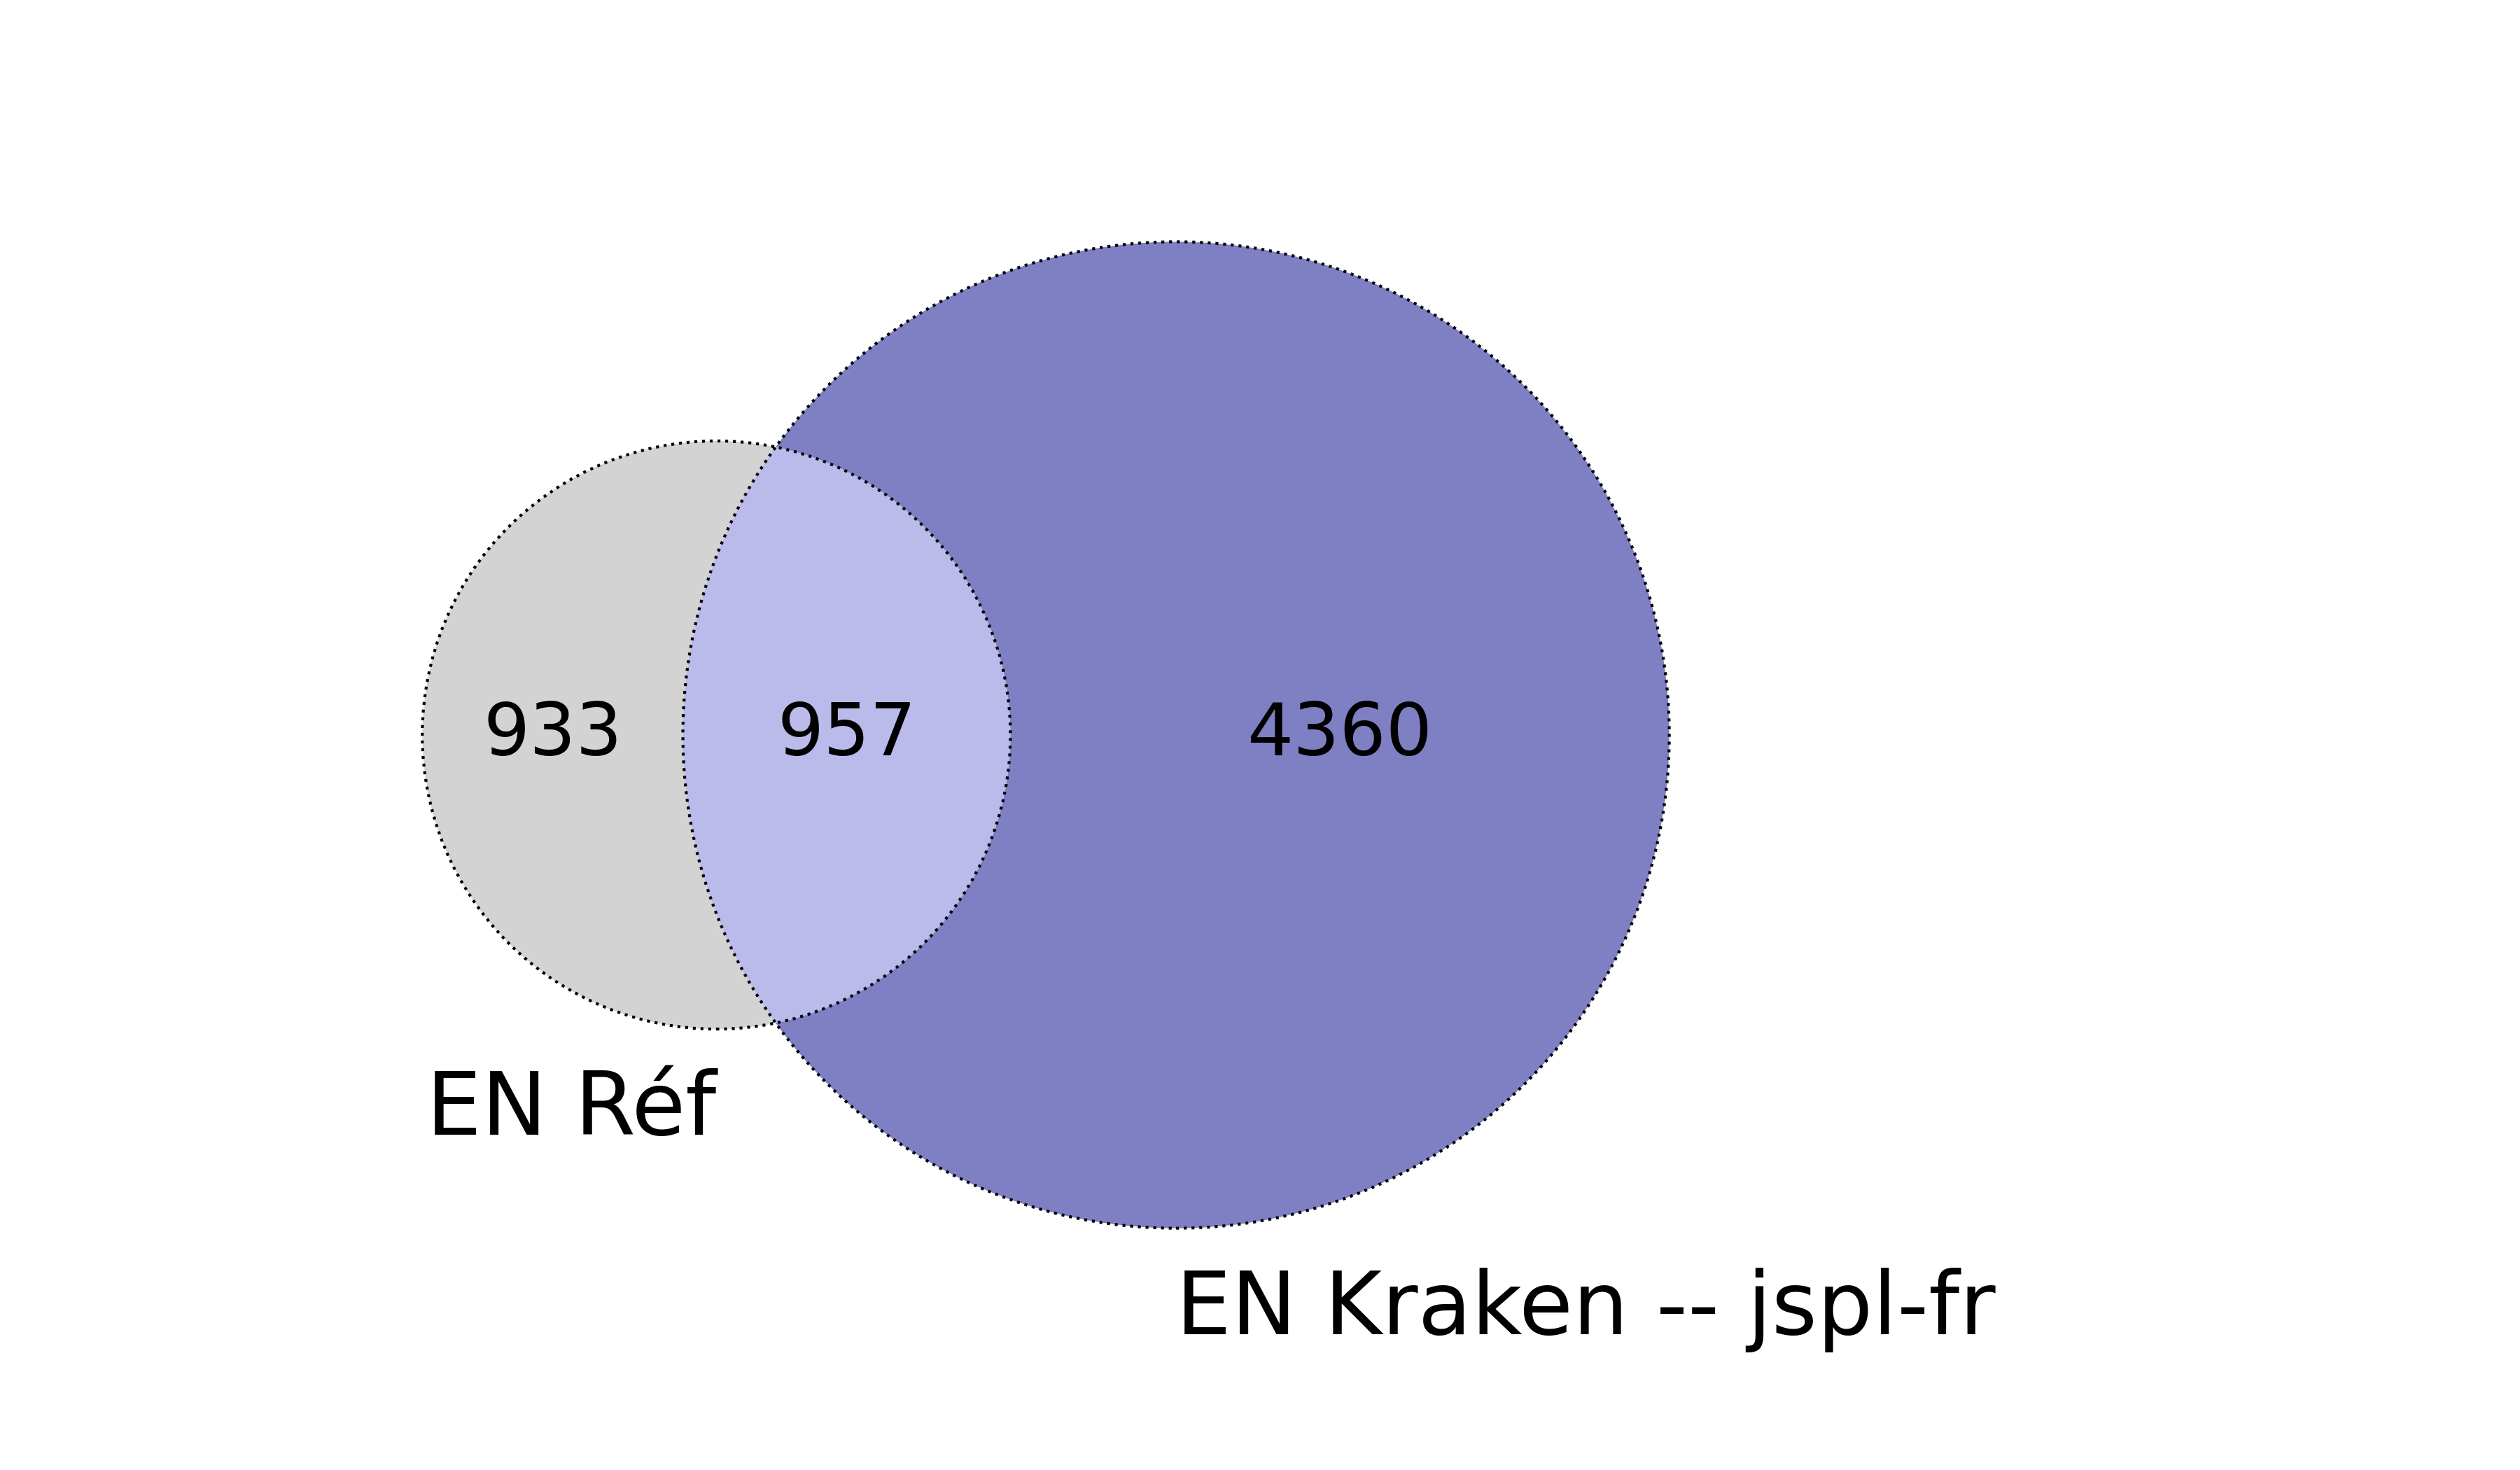
\includegraphics[width=1\textwidth]{IMAGES/INTERSECTIONS_GLOBALES/ELTeCFRA_Kraken -- jspl-fr_spacy-lg-concat_intersection.png} 
  \caption{Kraken--Jspll pretrain-fr --\texttt{spaCy\_lg}}
  \label{fig:ELTeCFRA_Kraken -- jspl-fr_spacy-lg-concat_intersection.png}
  \end{subfigure}
  \end{minipage}
  \begin{minipage}{6.5cm}
  \begin{subfigure}{1\textwidth}
  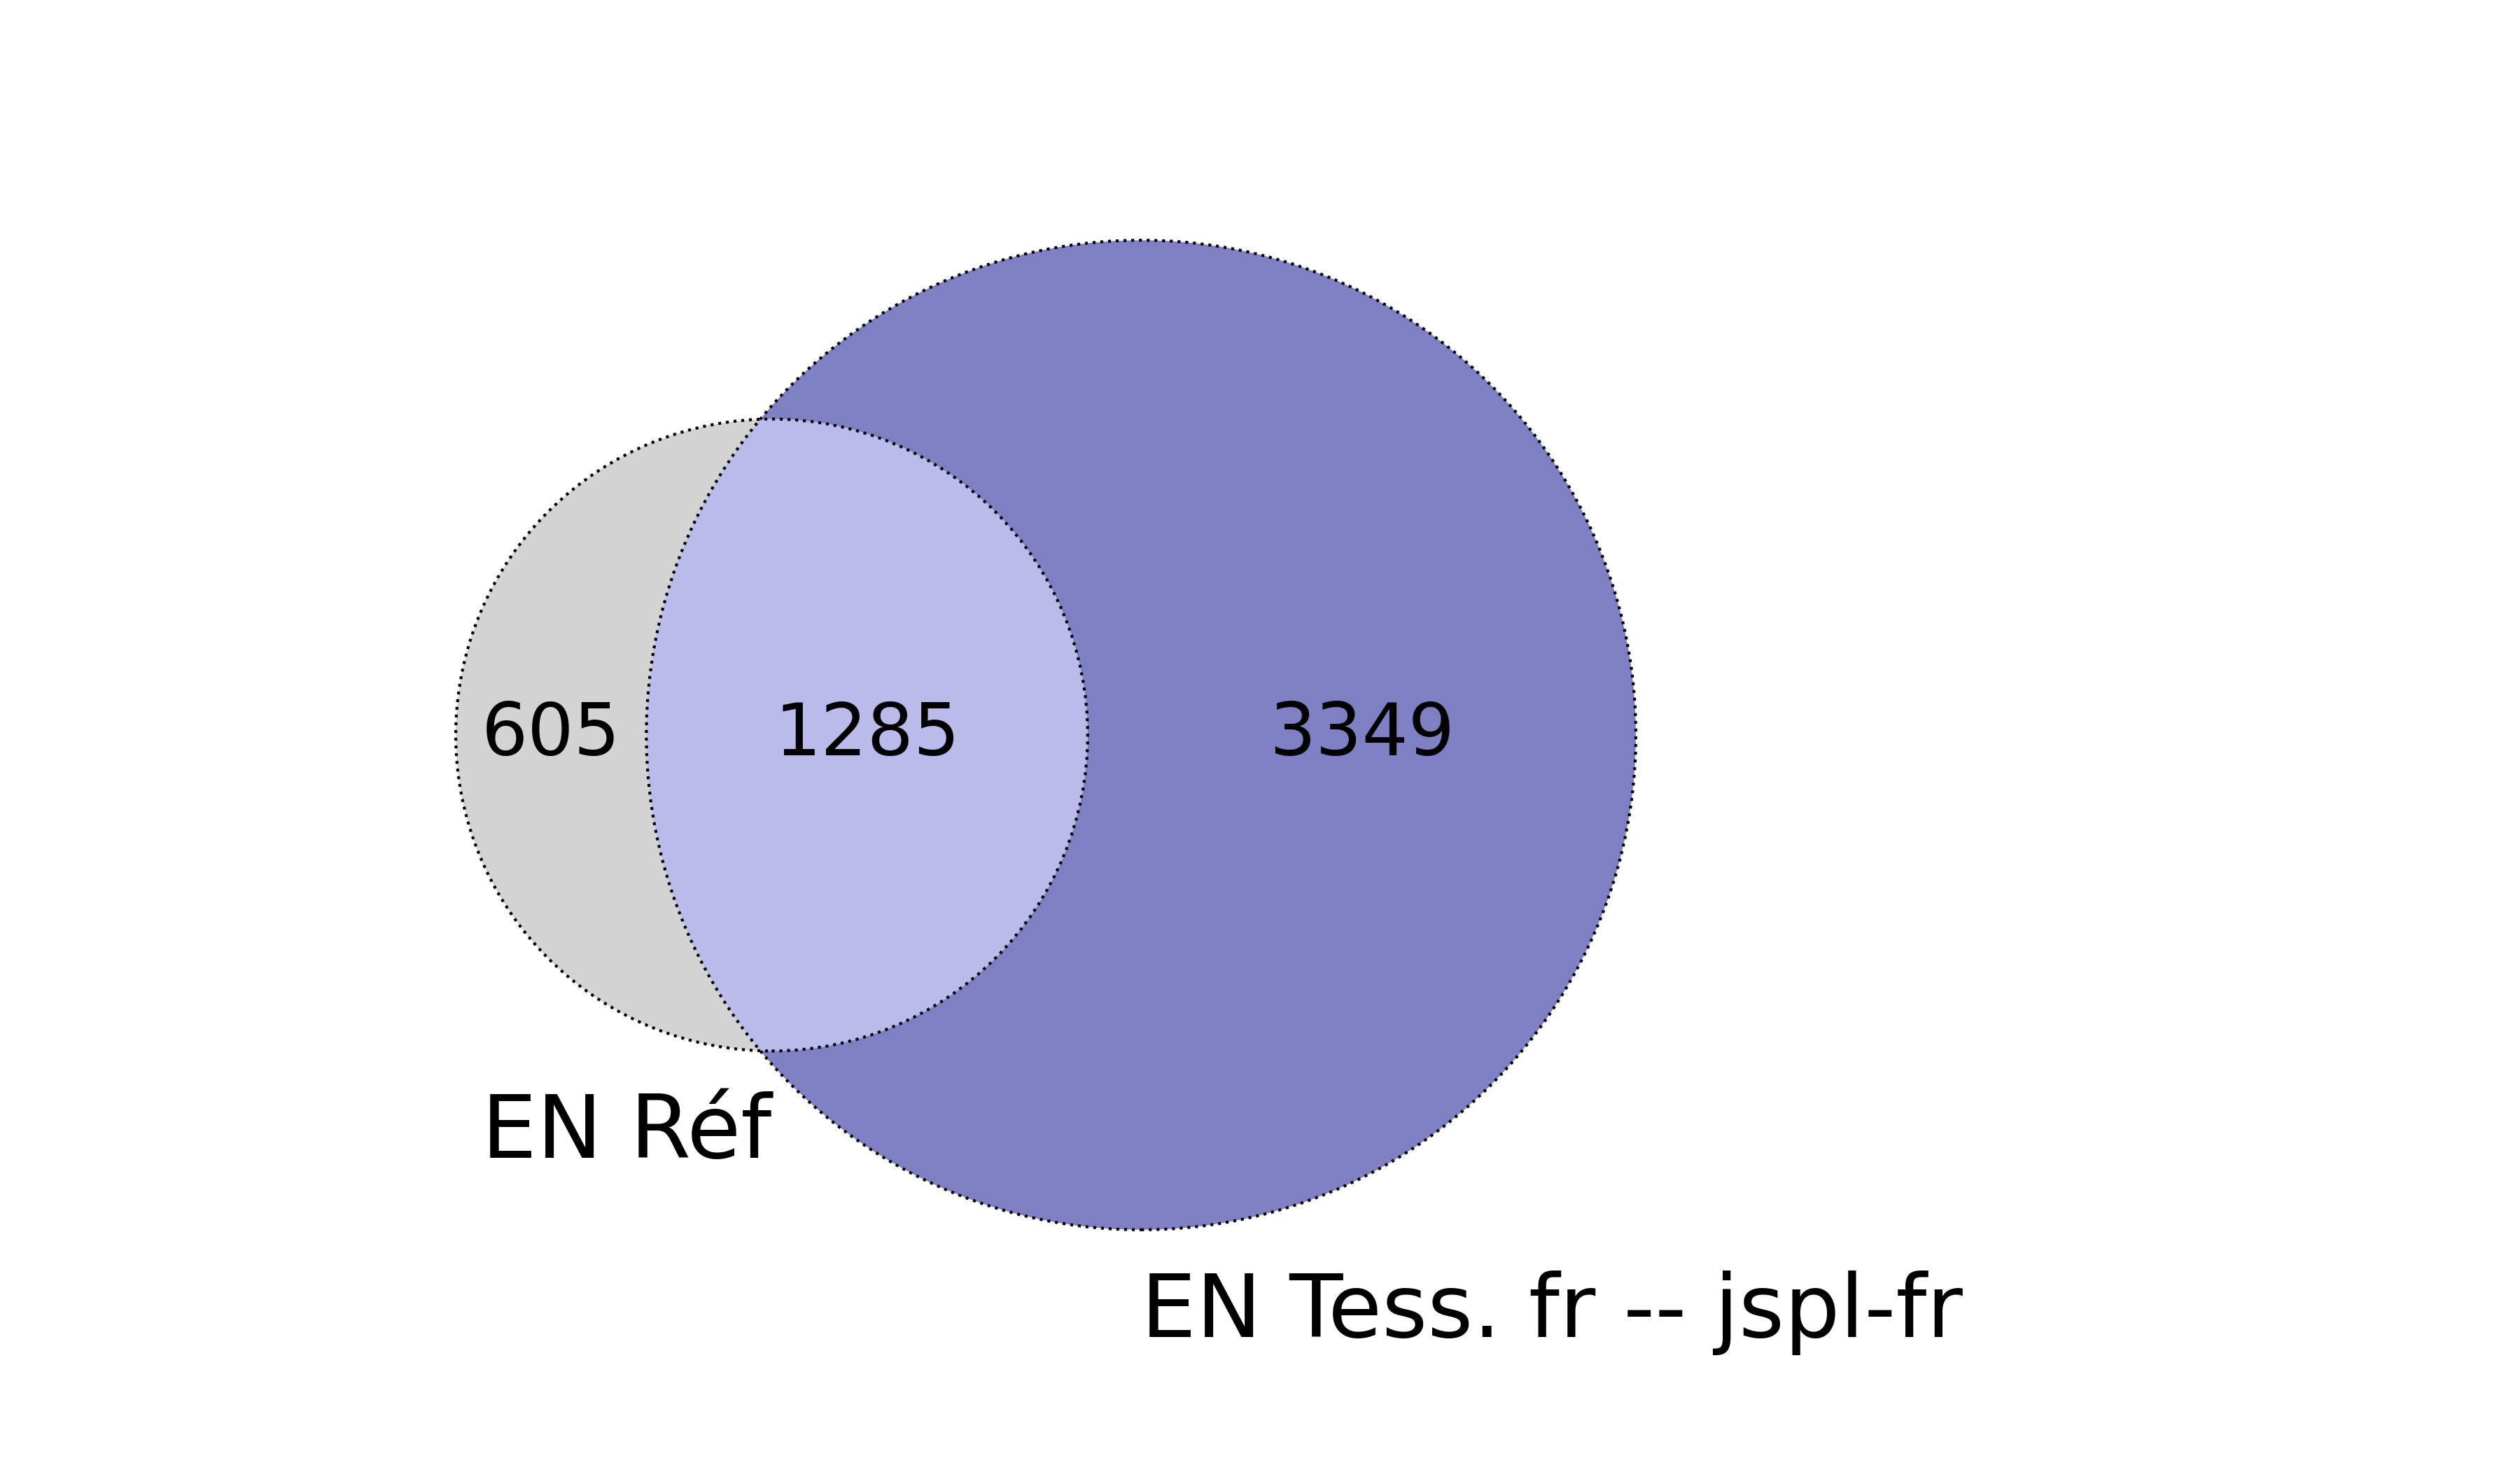
\includegraphics[width=1\textwidth]{IMAGES/INTERSECTIONS_GLOBALES/ELTeCFRA_Tess. fr -- jspl-fr_spacy-lg-concat_intersection.png} 
  \caption{Tess. fr.--Jspll pretrain-fr -- \texttt{spaCy\_lg}}
 \label{fig:ELTeCFRA_Tess. fr -- jspl-fr_spacy-lg-concat_intersection.png}
  \end{subfigure}
    \end{minipage}
\begin{minipage}{6.5cm}
  \begin{subfigure}{1\textwidth}
  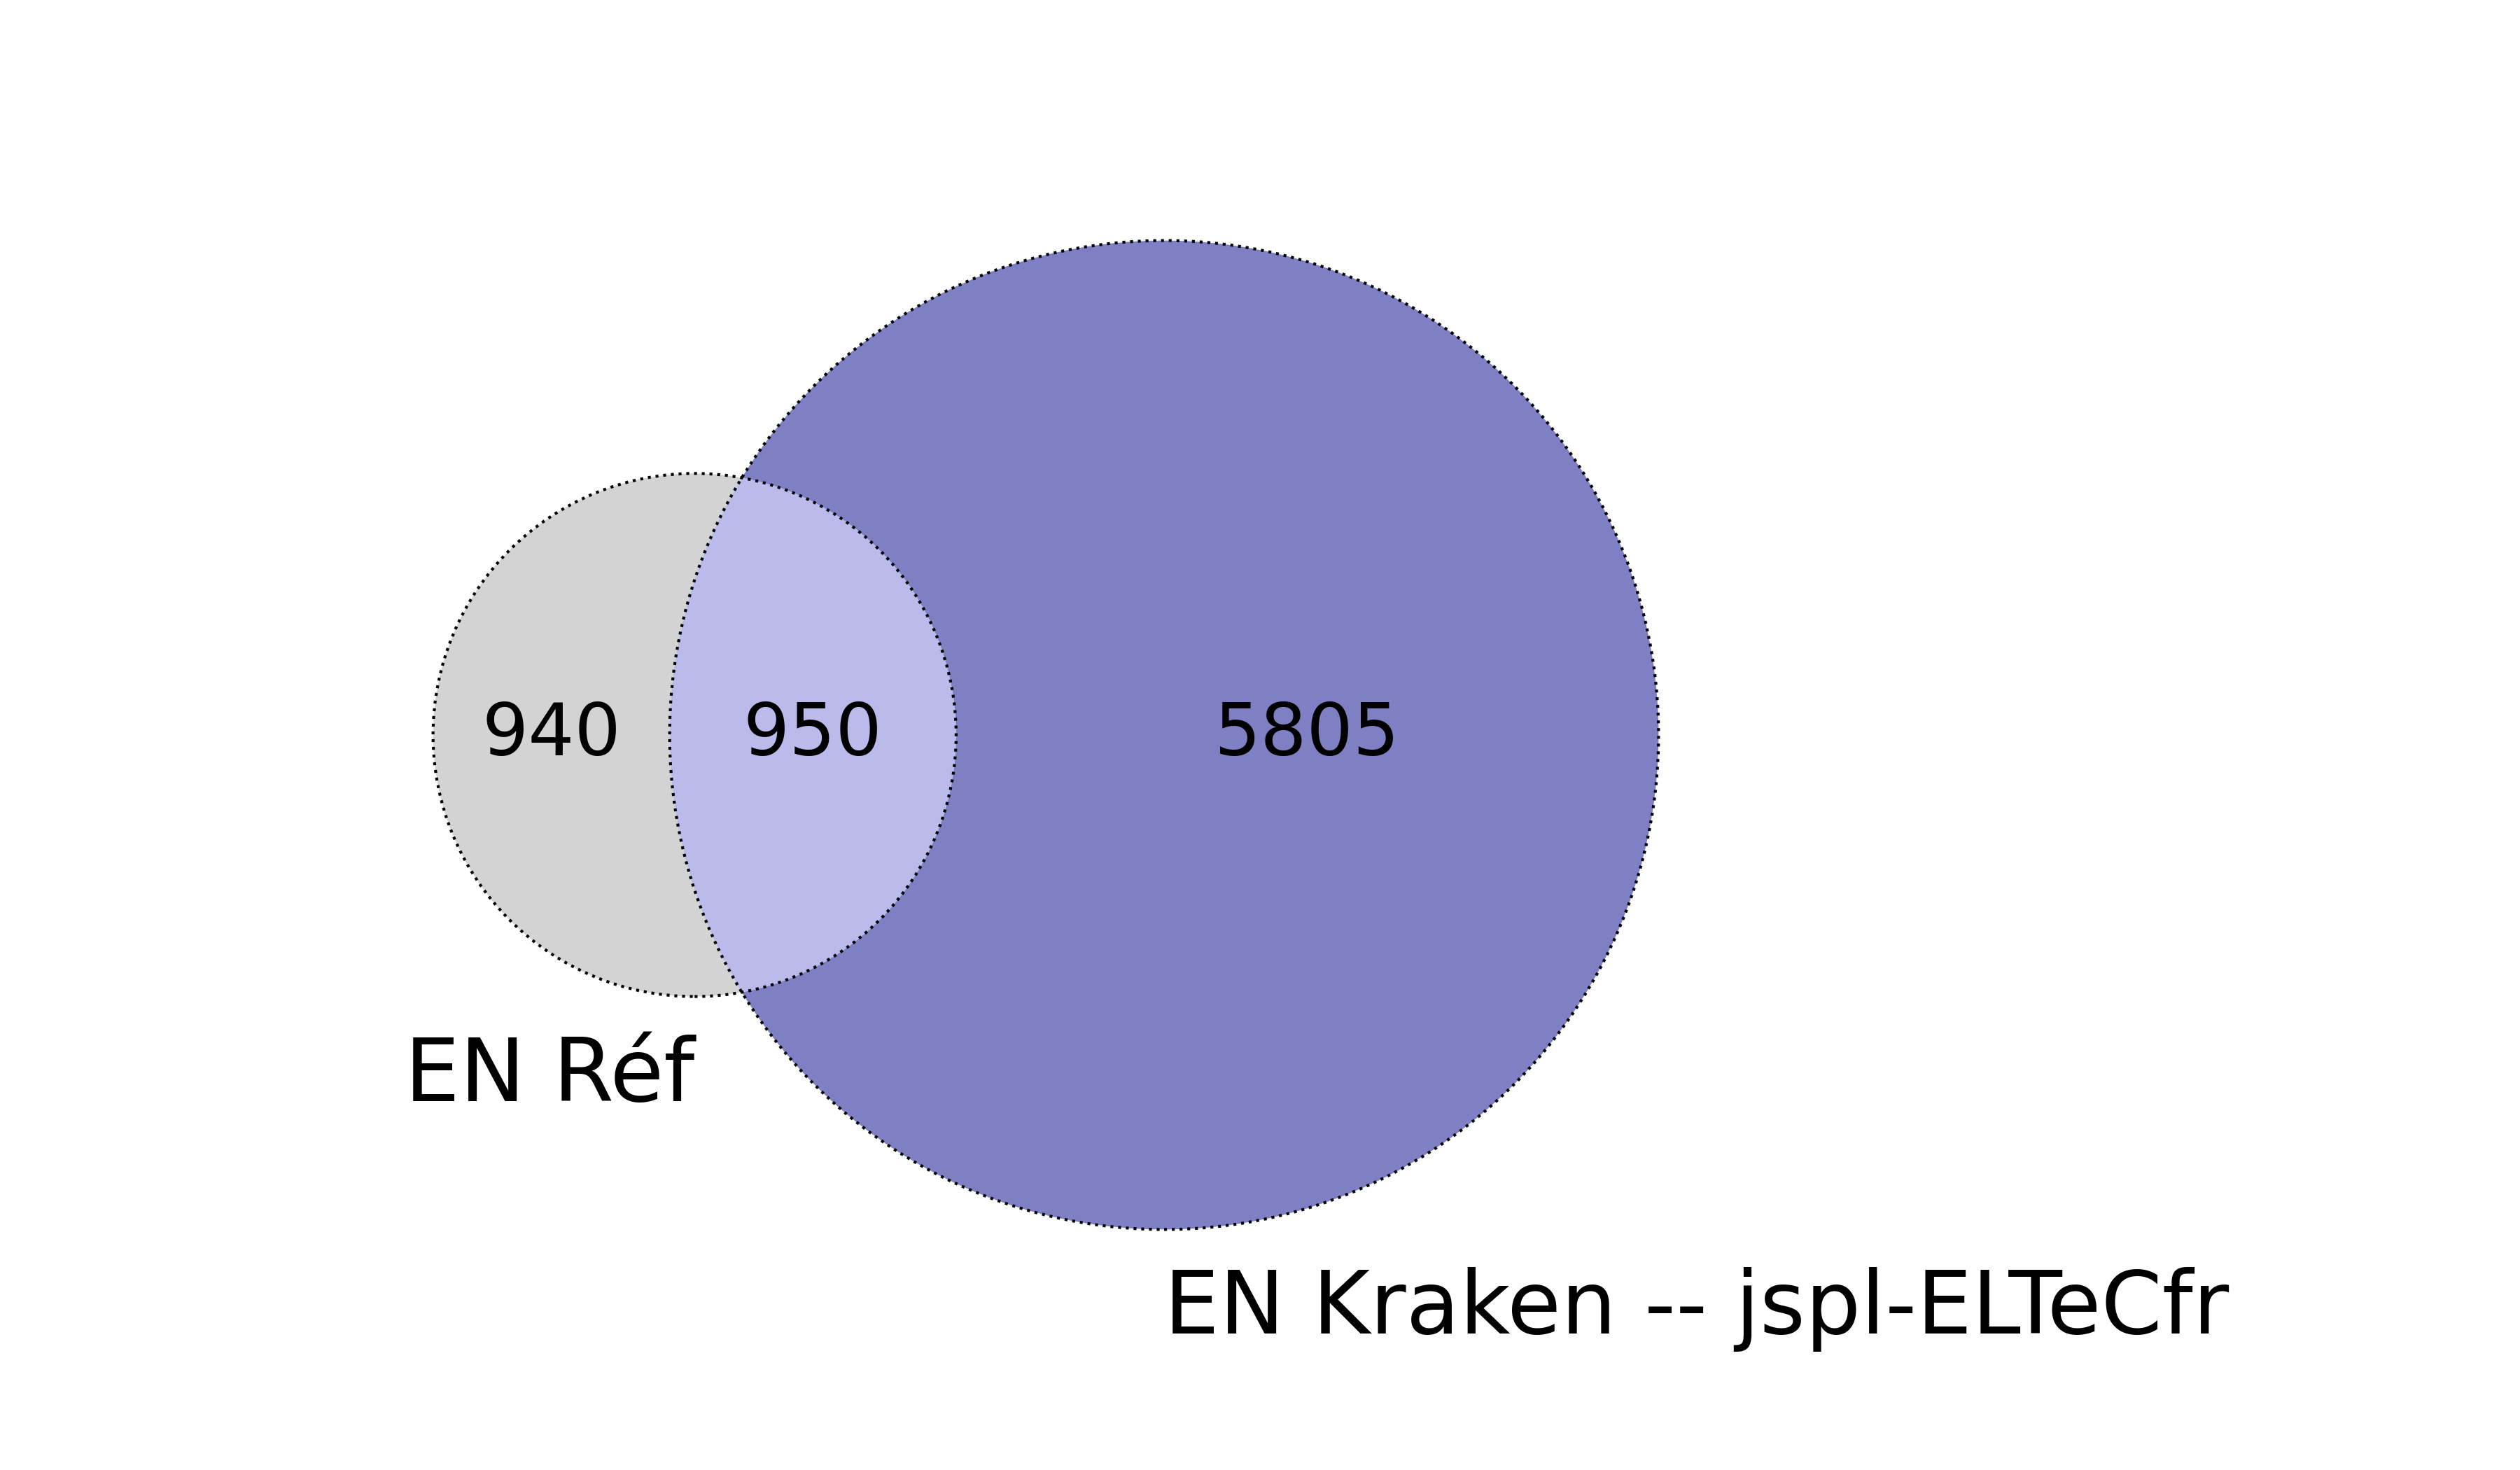
\includegraphics[width=1\textwidth]{IMAGES/INTERSECTIONS_GLOBALES/ELTeCFRA_Kraken -- jspl-ELTeCfr_spacy-lg-concat_intersection.png} 
  \caption{Kraken--Jspll ELTeC-fr -- \texttt{spaCy\_lg}}
  \label{fig:ELTeCFRA_Kraken -- jspl-ELTeCfr_spacy-lg-concat_intersection}
  \end{subfigure}
  \end{minipage}
  \begin{minipage}{6.5cm}
  \begin{subfigure}{1\textwidth}
  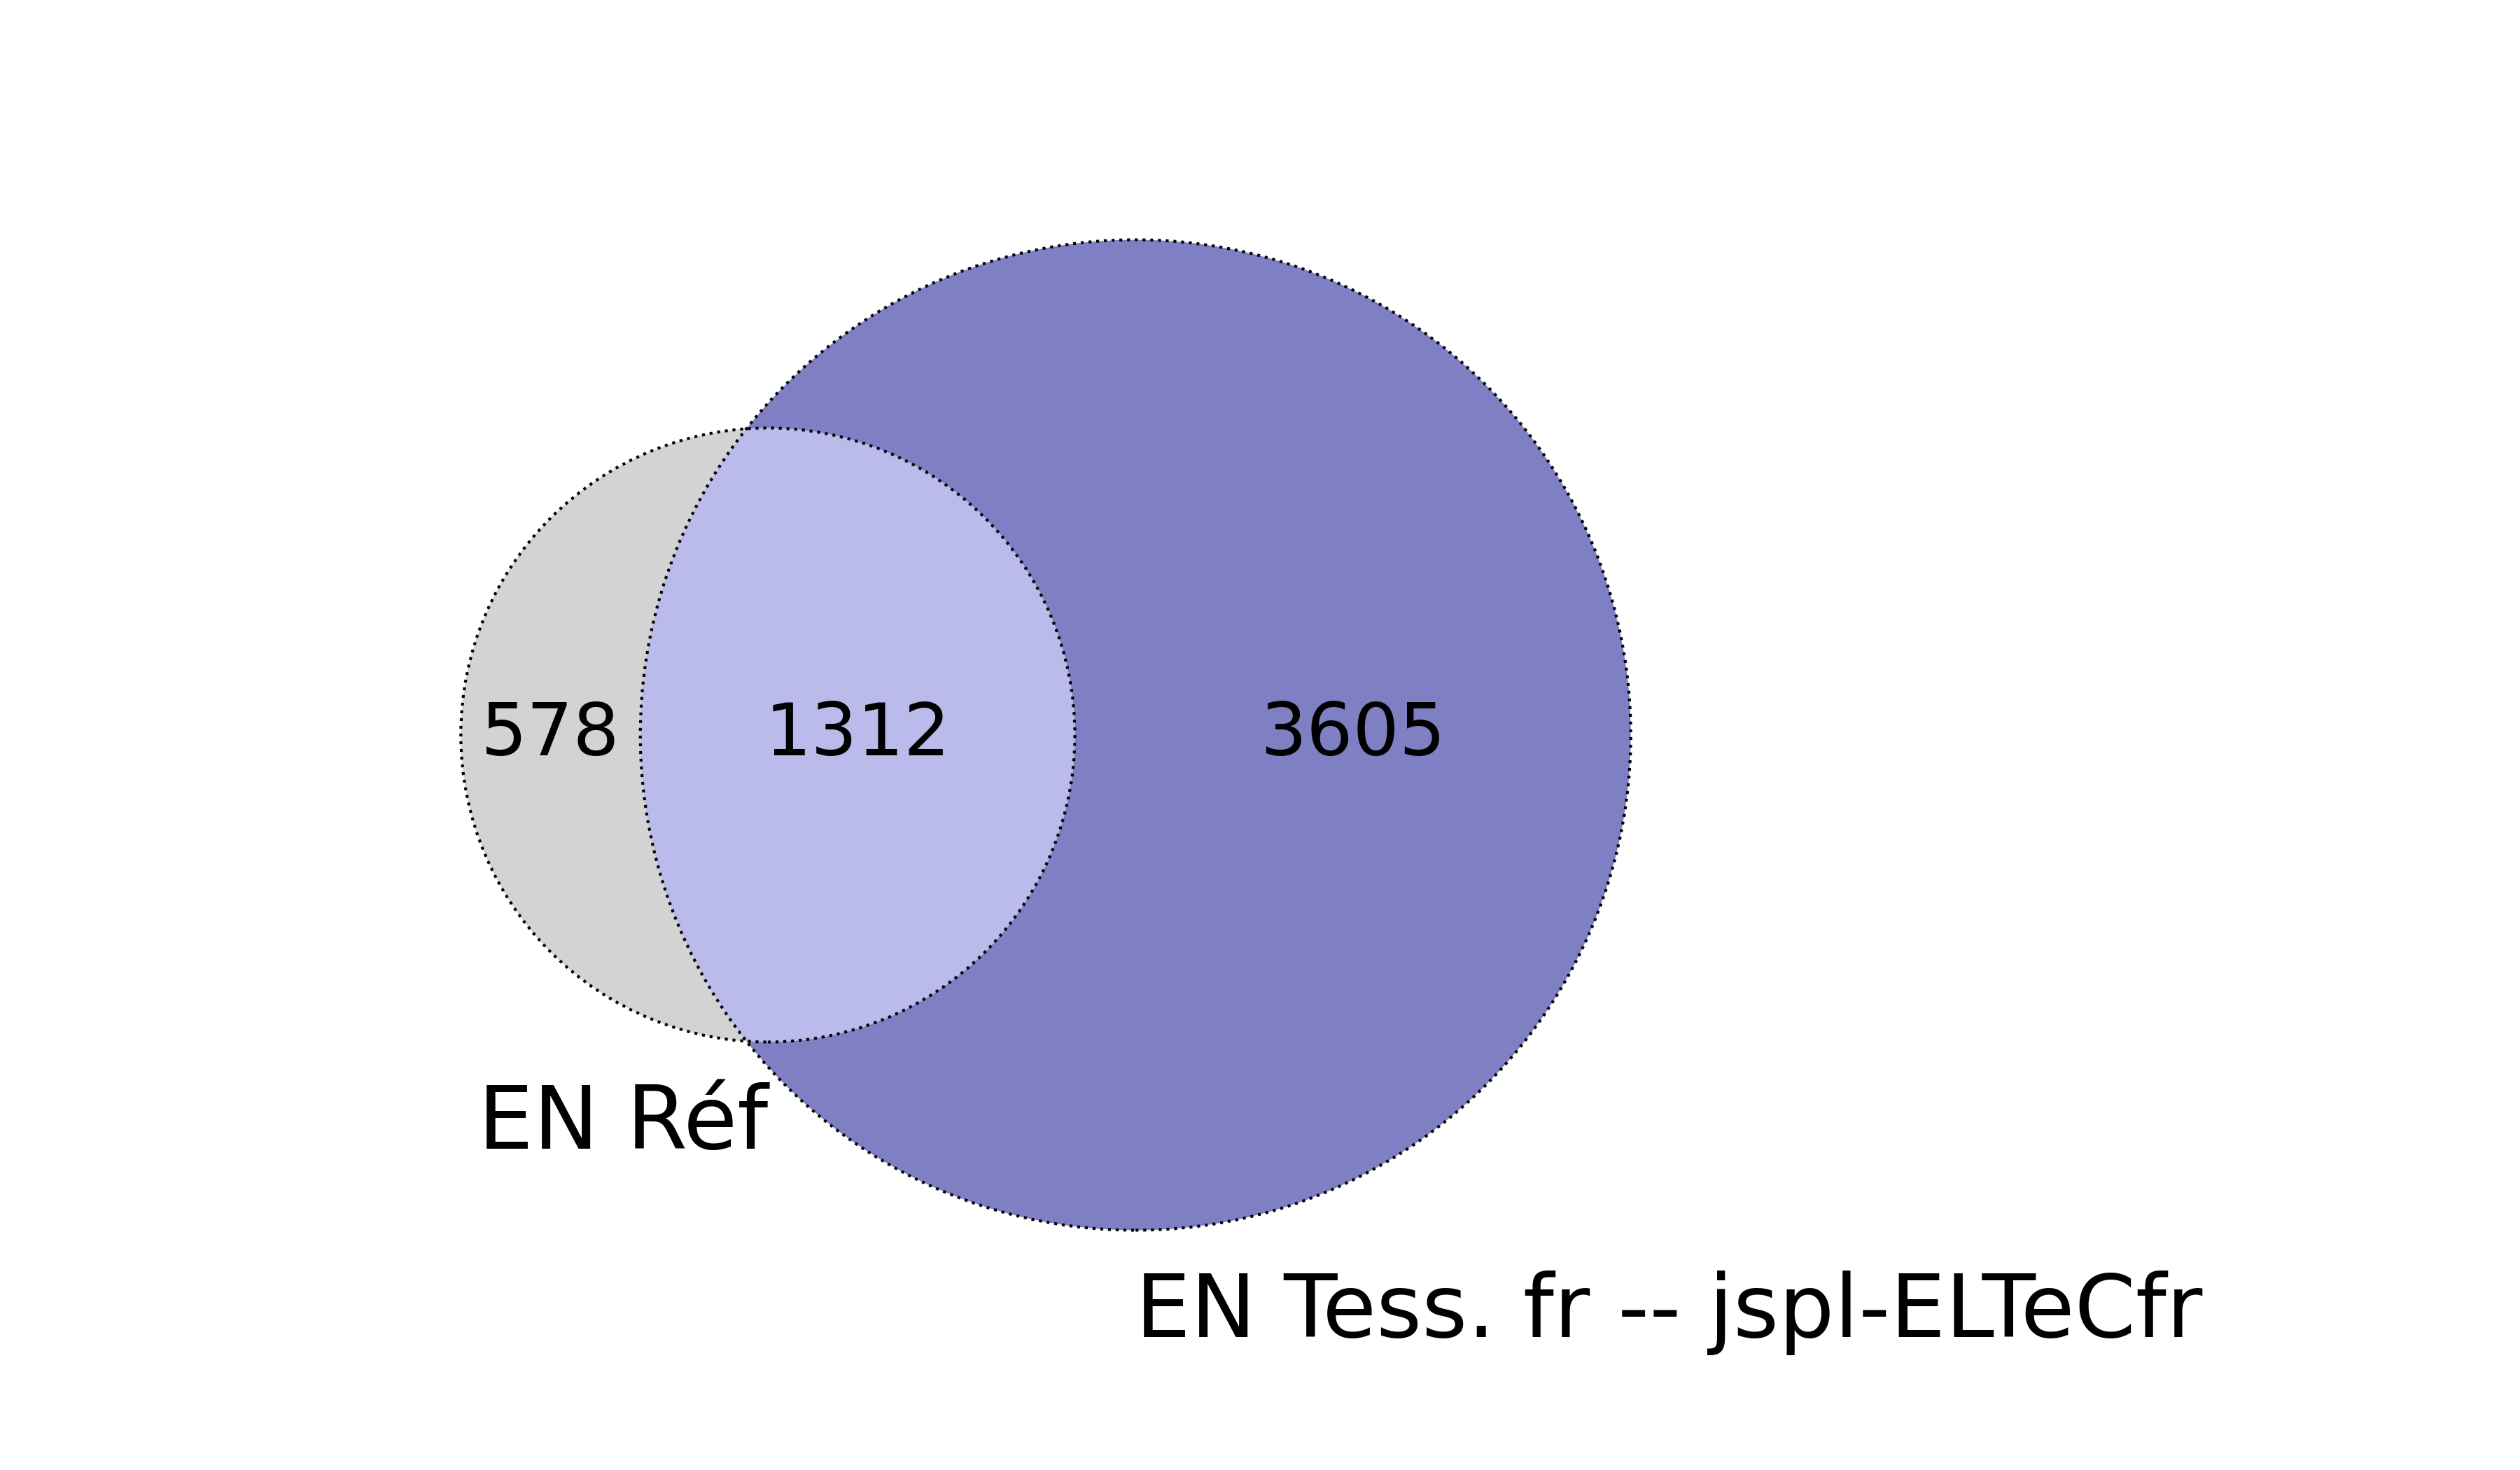
\includegraphics[width=1\textwidth]{IMAGES/INTERSECTIONS_GLOBALES/ELTeCFRA_Tess. fr -- jspl-ELTeCfr_spacy-lg-concat_intersection.png} % nouvelle figure ici avec Tess. fr. corrigé avec spaCy_lg
  \caption{Tess. fr.--Jspll ELTeC-fr -- \texttt{spaCy\_lg}}
  \label{fig:ELTeCFRA_Tess -- jspl-ELTeCFR_spacy-lg-concat_intersection}
  \end{subfigure}
    \end{minipage}
%\caption{Intersections pour les configurations (\ref{fig:ELTeCFRA_Kraken -- jspl-fr_spacy-lg-concat_intersection.png
%}-\ref{fig:ELTeCFRA_Tess -- spacy-lg-concat_intersection}) Kraken-\texttt{spaCy\_lg} et Tess. fr.-\texttt{spaCy\_lg} non corrigées, et (\ref{fig:ELTeCFRA_Kraken -- jspl-ELTeCfr_spacy-lg-concat_intersection}-\ref{fig:ELTeCFRA_Tess -- jspl-ELTeCFR_spacy-lg-concat_intersection}) les configurations équivalentes corrigées avec JamSpell (modèle ELTeC), pour le corpus ELTeC français.}
\caption{Intersections pour les configurations Kraken et Tess. fr. corrigées par JamSpell pré-entraîné et modèle ELTeC, \texttt{spaCy\_lg} sur le corpus ELTeC français.}
\label{fig:intersection_globale-kraken}
\end{figure}

Ce fait peut être lu à l'aune des observations présentées dans le tableau \ref{tab:typologie_erreurs-corr_ELTeCEng} rapportant la typologie des erreurs de corrections. Autrement dit, la correction automatique ne transforme pas toutes les EN contaminées par la ROC en EN corrigées strictement associables avec les EN du groupe de référence. Ainsi les BOIC (``Morlincourt'' qui devient ``Martincourt''), se cumulant aux EN contaminées non corrigées MOI (``Morlincourtl'' qui reste ``Morlincourtl''), n'améliorent pas les résultats obtenus par calcul des intersections. Il semble que pour les corpus ELTeC français, anglais et portugais et celui de la TGB la correction automatique avec le modèle entraîné sur une partie de chaque corpus ELTeC fasse perdre 5\% des EN dans l'intersection avec Kraken et 10\% avec Tesseract, alors que concernant les modèles pré-entraînés on perd 3\% avec Kraken et 9\% avec Tesseract. Cette expérience est l'occasion de démontrer les limites d'une évaluation stricte de la REN sur des textes bruités et leurs versions corrigées. Nos observations manuelles montrent que les contaminations de la ROC d'une part et de la correction automatique d'autre part ne sont pas véritablement un frein à la REN, mais l'évaluation automatique des résultats n'est pas triviale.

%%%%%%%%%%%%%%%% Ancienne figure avec les intersections pour la config Tess-spaCy_lg corrigées avec le modèle pré-entraîné de JamSpell et le modèle ELTeC, pour le corpus ELTeC fr %%%%%%%%%%%%%%%%%%

%\begin{figure}[h!]
%%    \begin{minipage}{7cm}
%%  \begin{subfigure}{1\textwidth}
%%  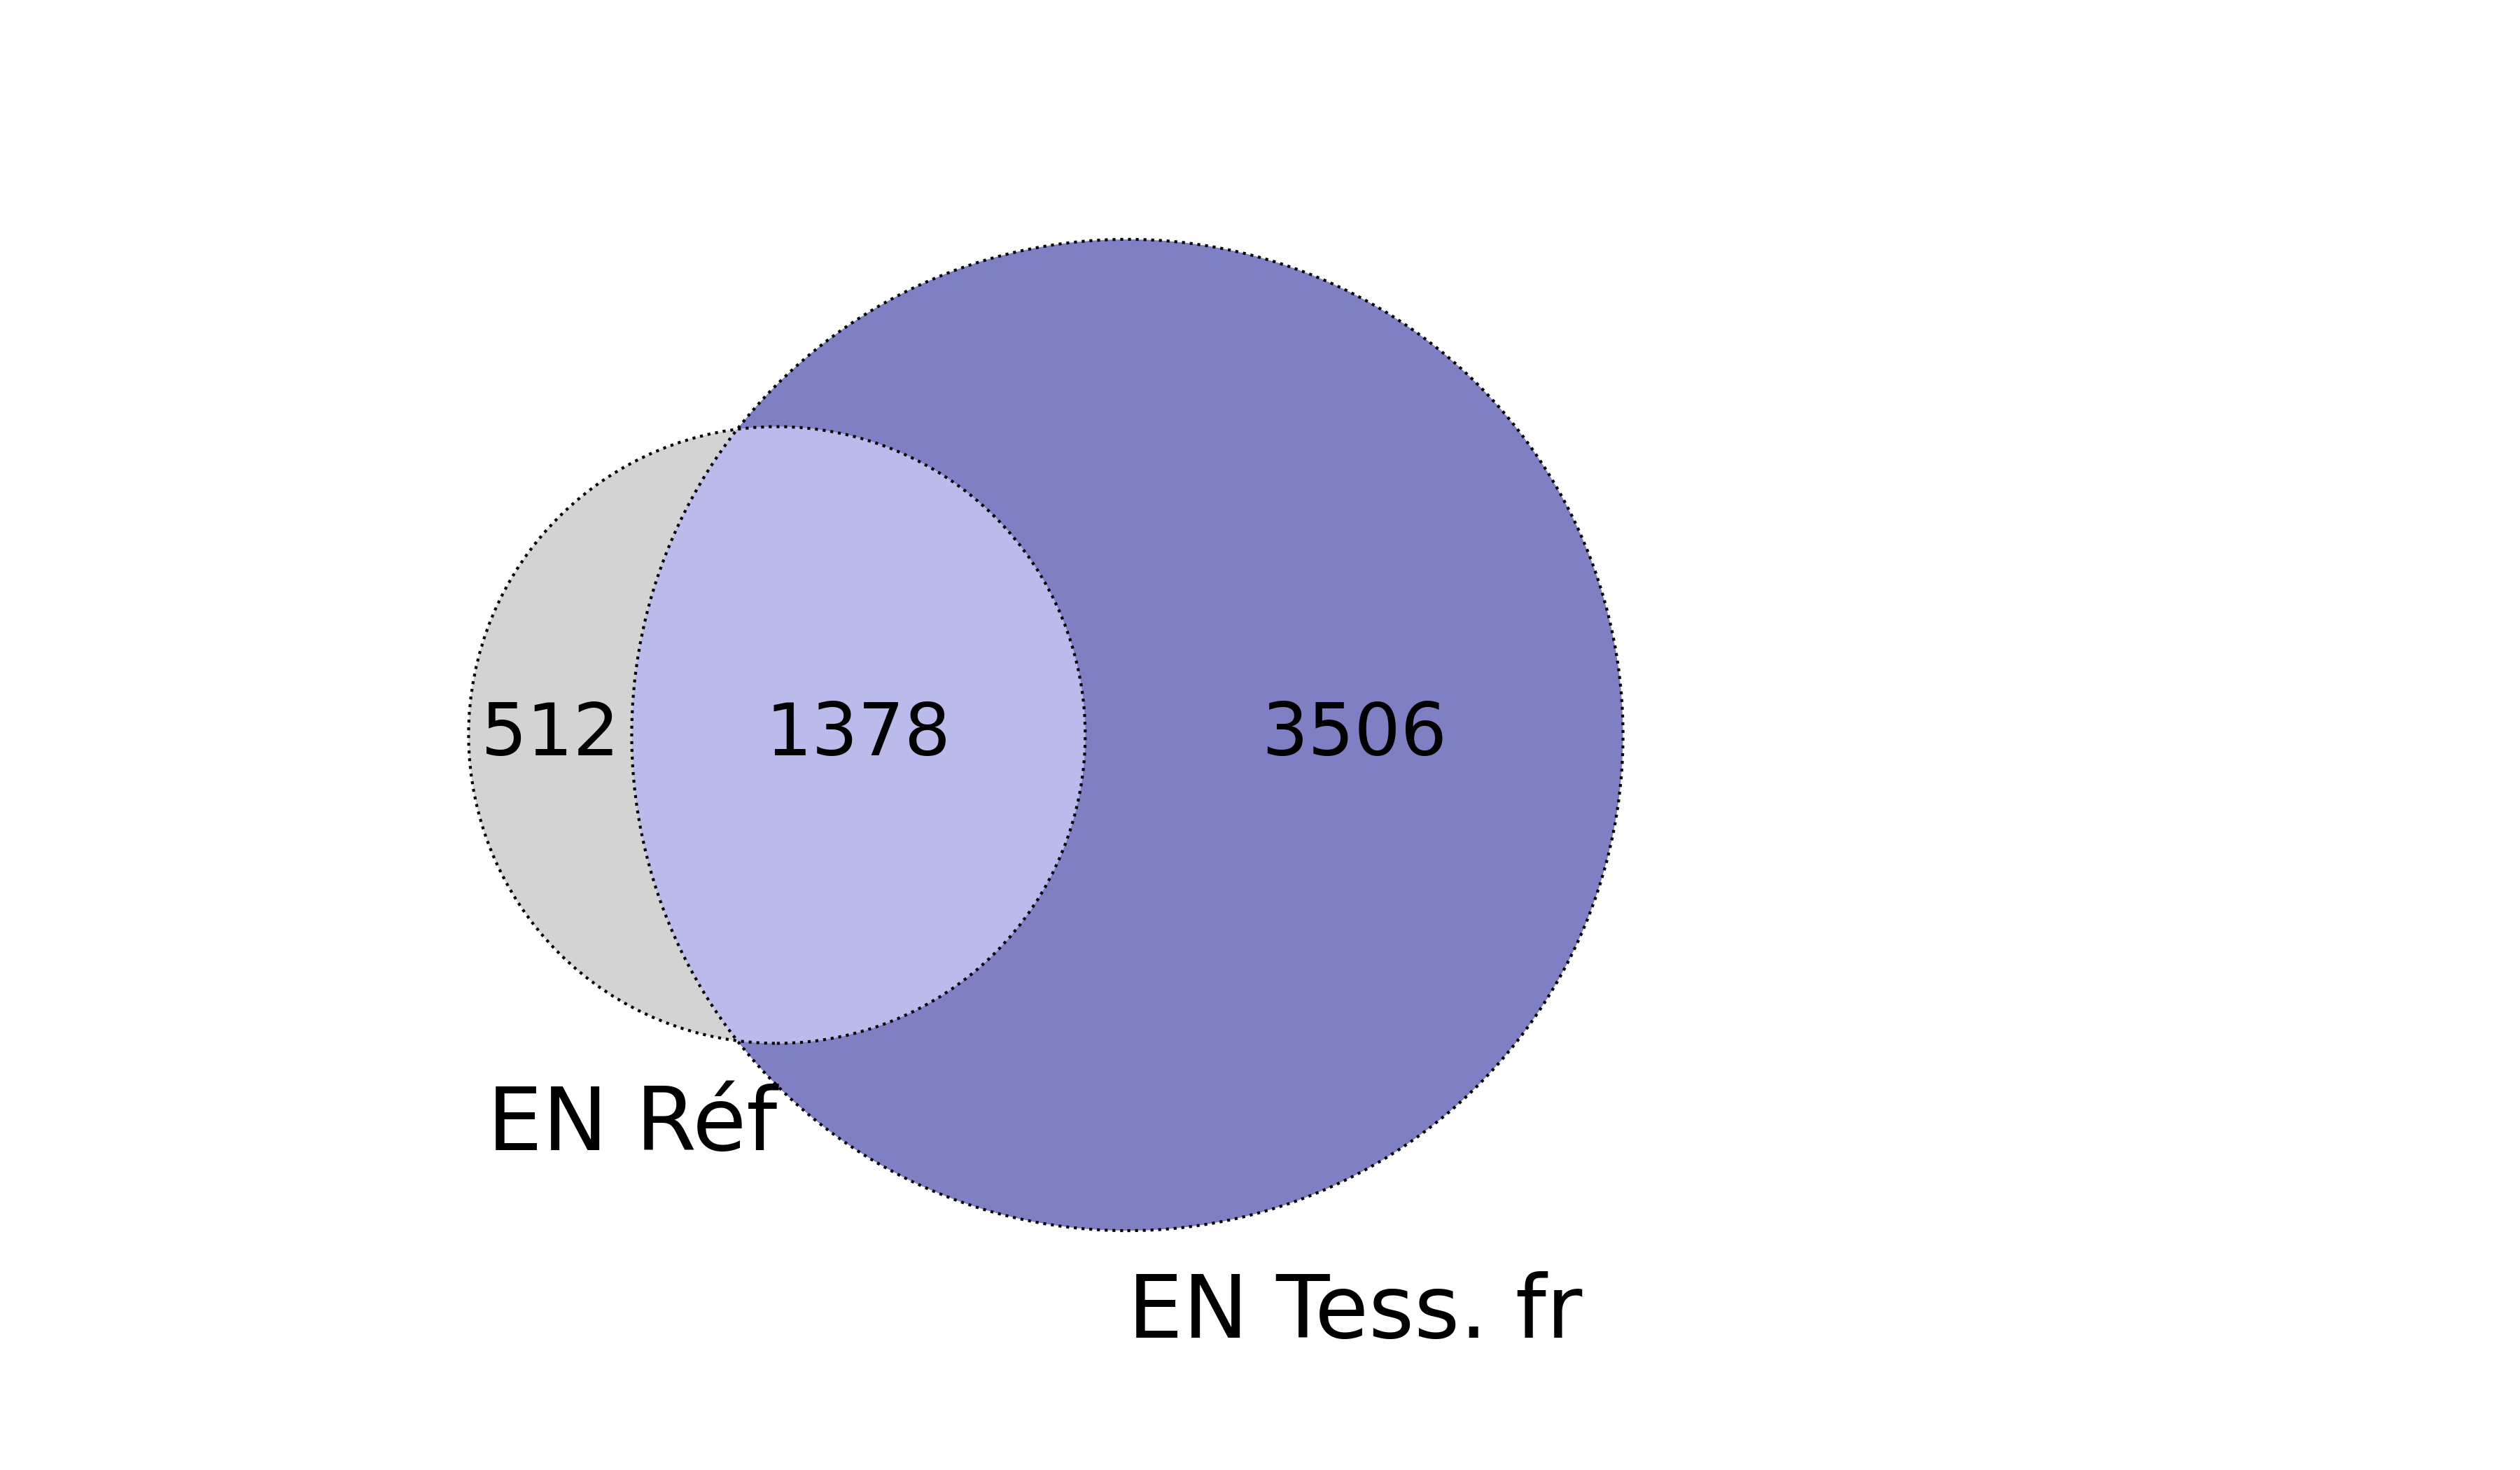
\includegraphics[width=1\textwidth]{IMAGES/INTERSECTIONS_GLOBALES/ELTeCFRA_Tess. fr_spacy-lg-concat_intersection.png} 
%%  \caption{Tess. fr. --\texttt{spaCy\_lg}}
%%  \label{fig:ELTeCFRA_Tess. fr_spacy-lg-concat_intersection}
%%  \end{subfigure}
%%  \end{minipage}
%%  \begin{minipage}{7cm}
%%  \begin{subfigure}{1\textwidth}
%%  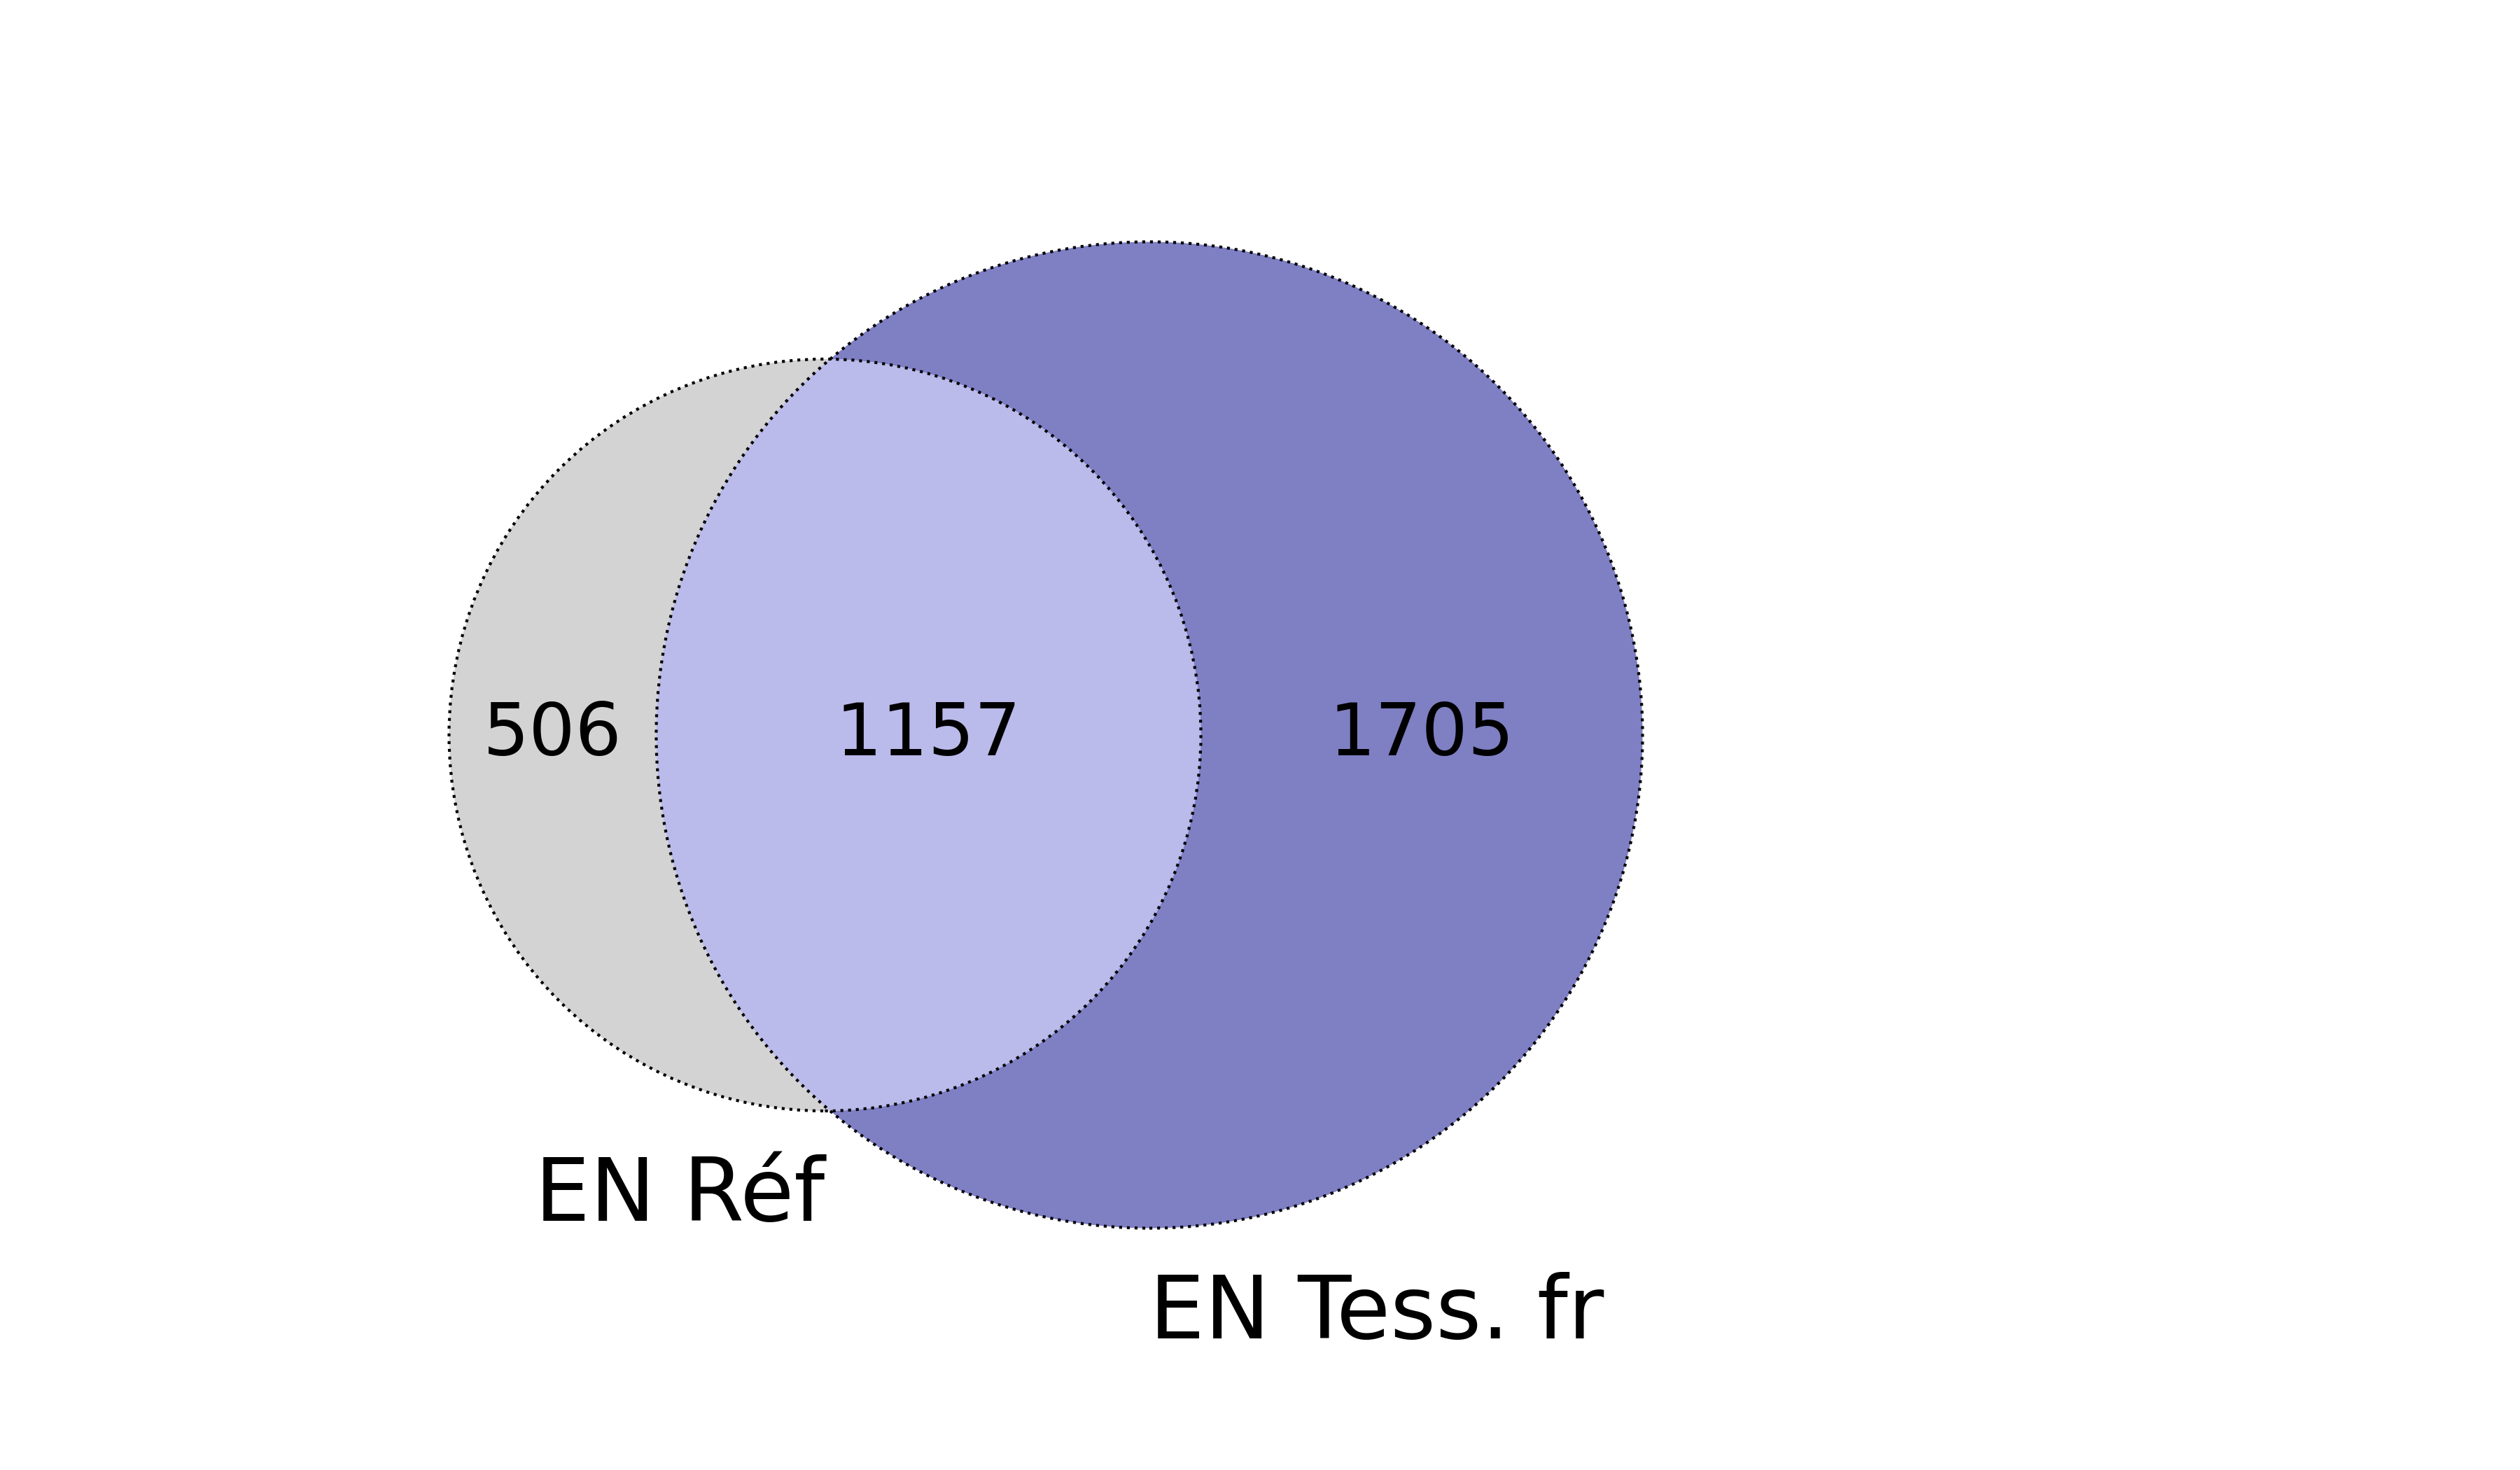
\includegraphics[width=1\textwidth]{IMAGES/INTERSECTIONS_GLOBALES/ELTeCFRA_Tess. fr_stanza-concat_intersection.png}
%%  \caption{Tess. fr. -- \texttt{stanza}}
%% % \label{fig:ELTeCFRA_Tess. fr_stanza-concat_intersection}
%%  \end{subfigure}
%%    \end{minipage}
%%\begin{minipage}{7cm}
%%  \begin{subfigure}{1\textwidth}
%%  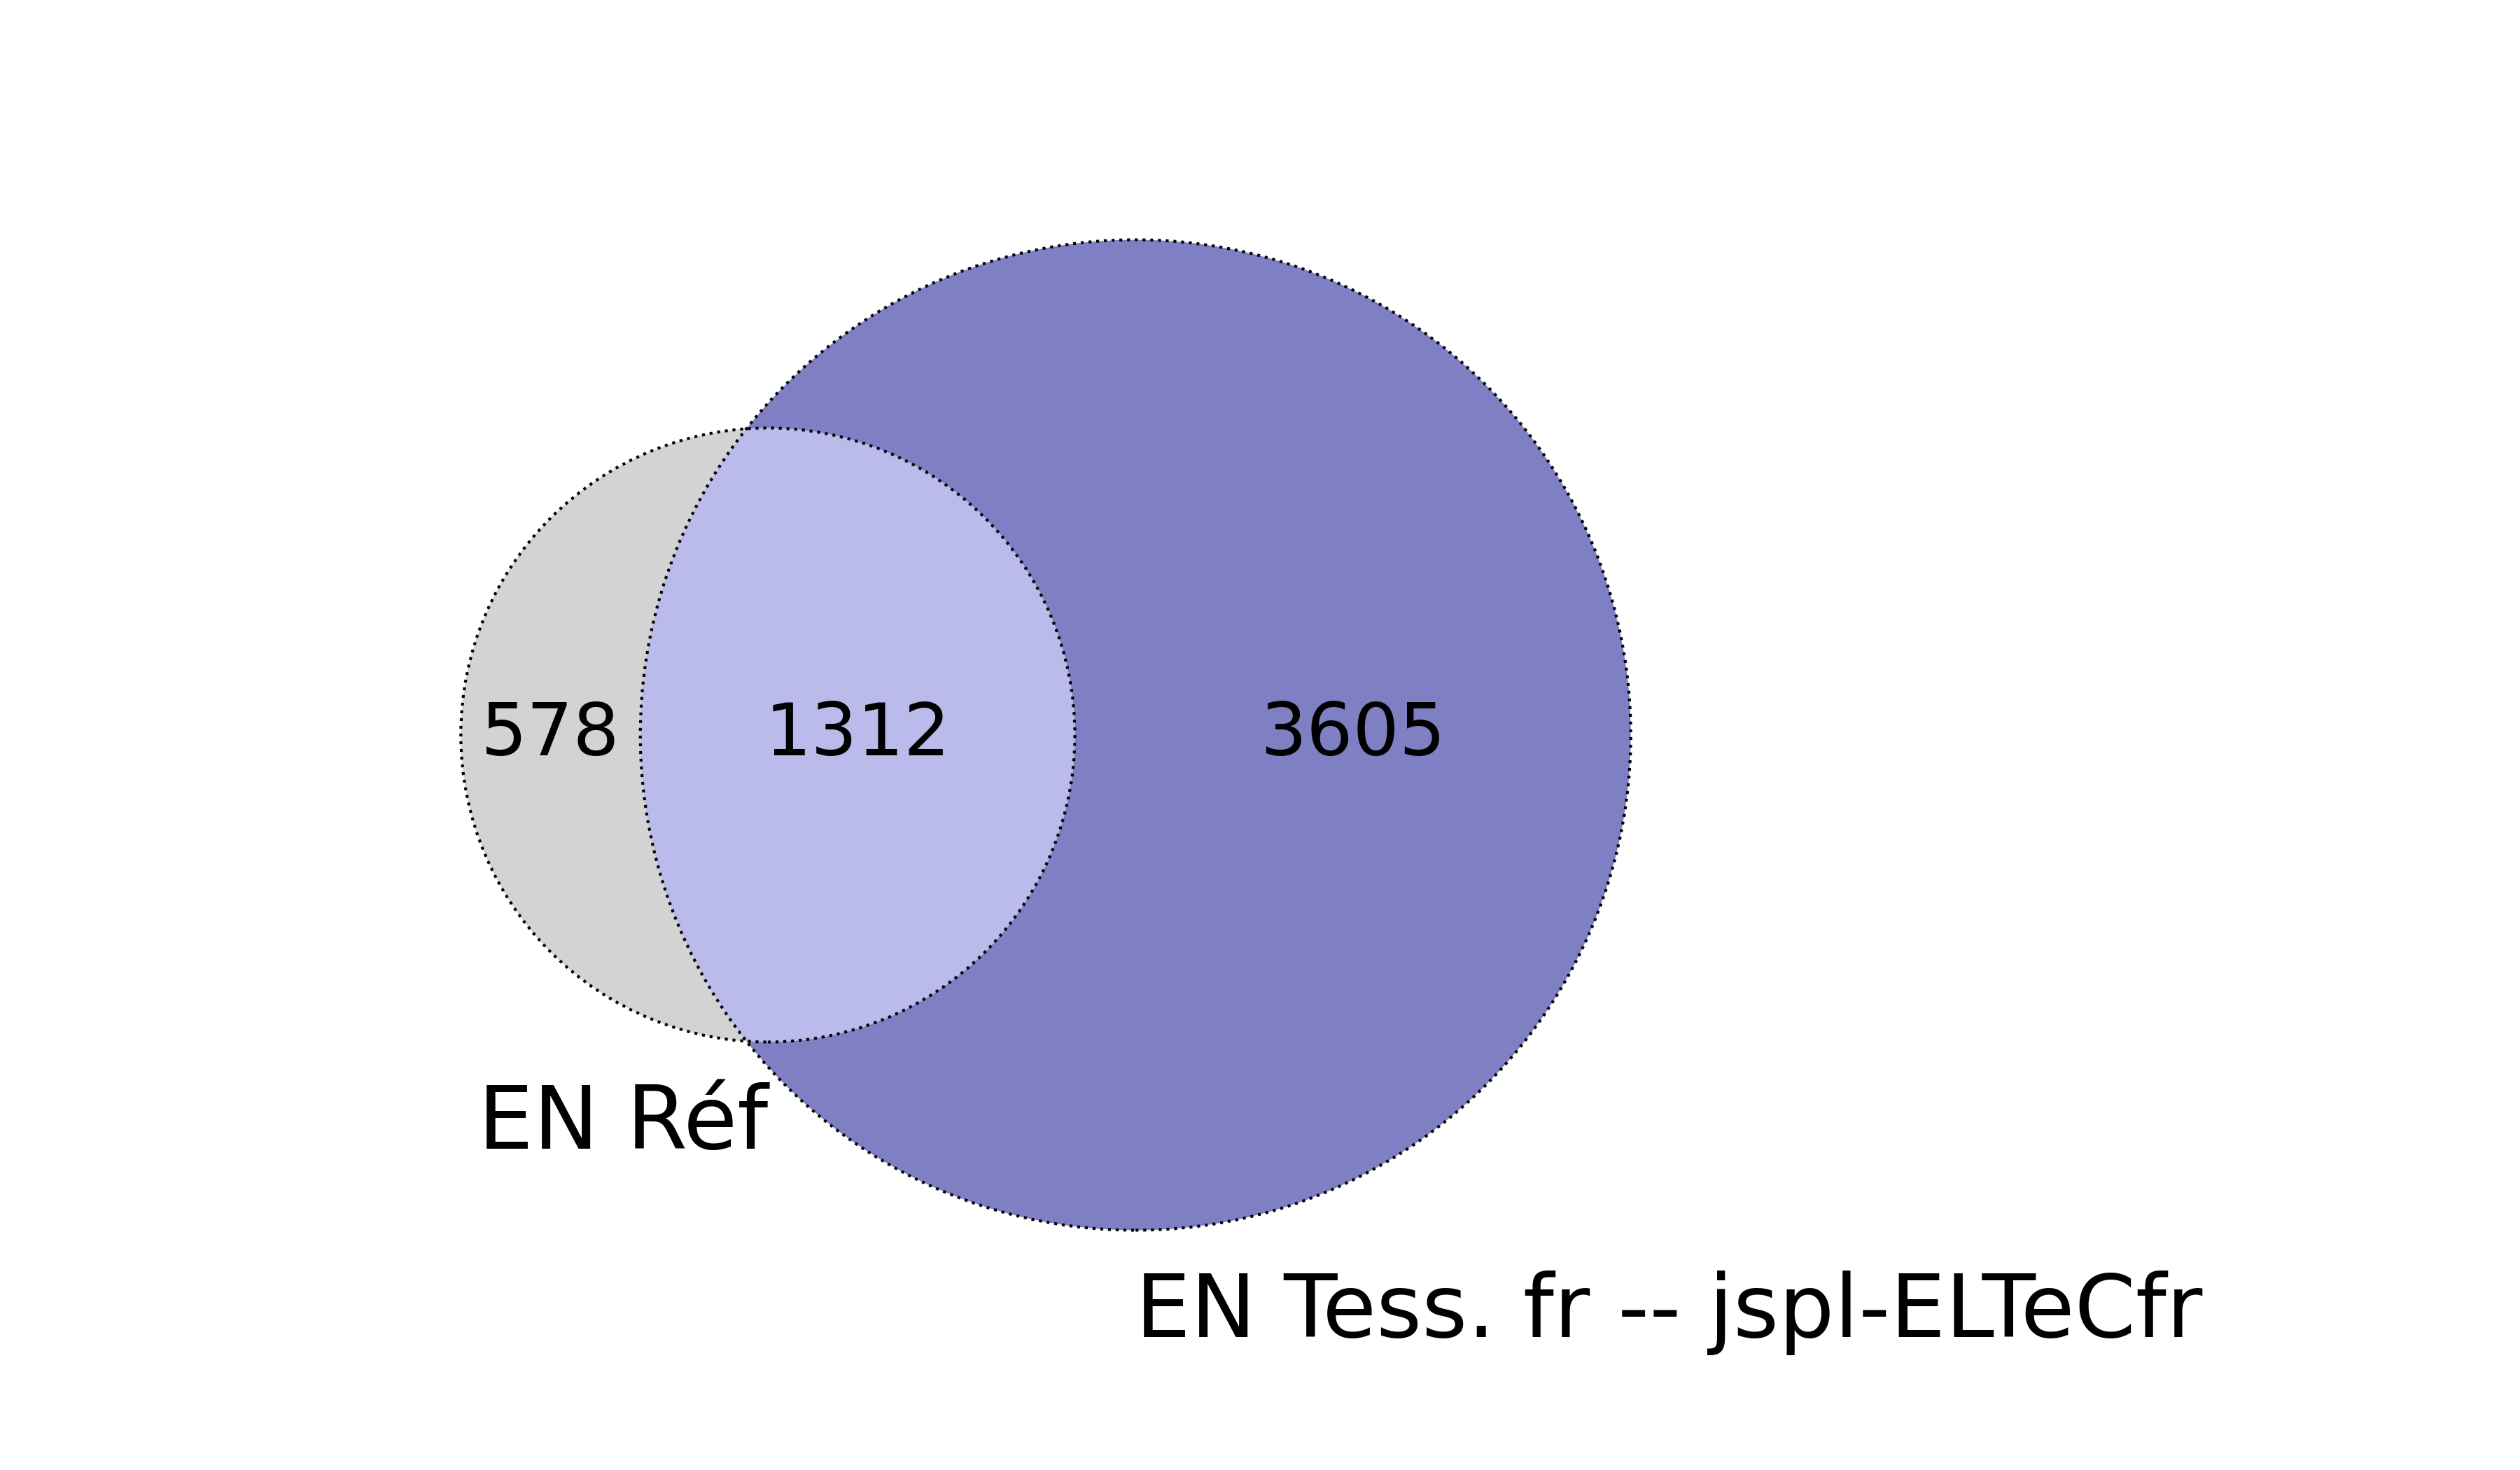
\includegraphics[width=1\textwidth]{IMAGES/INTERSECTIONS_GLOBALES/ELTeCFRA_Tess. fr -- jspl-ELTeCfr_spacy-lg-concat_intersection.png} 
%%  \caption{Tess. fr. corrigé -- \texttt{spaCy\_lg}}
%%  \label{fig:ELTeCFRA_Tess. fr -- jspl-ELTeCfr_spacy-lg-concat_intersection}
%%  \end{subfigure}
%%  \end{minipage}
%  \begin{minipage}{7cm}
%  \begin{subfigure}{1\textwidth}
%  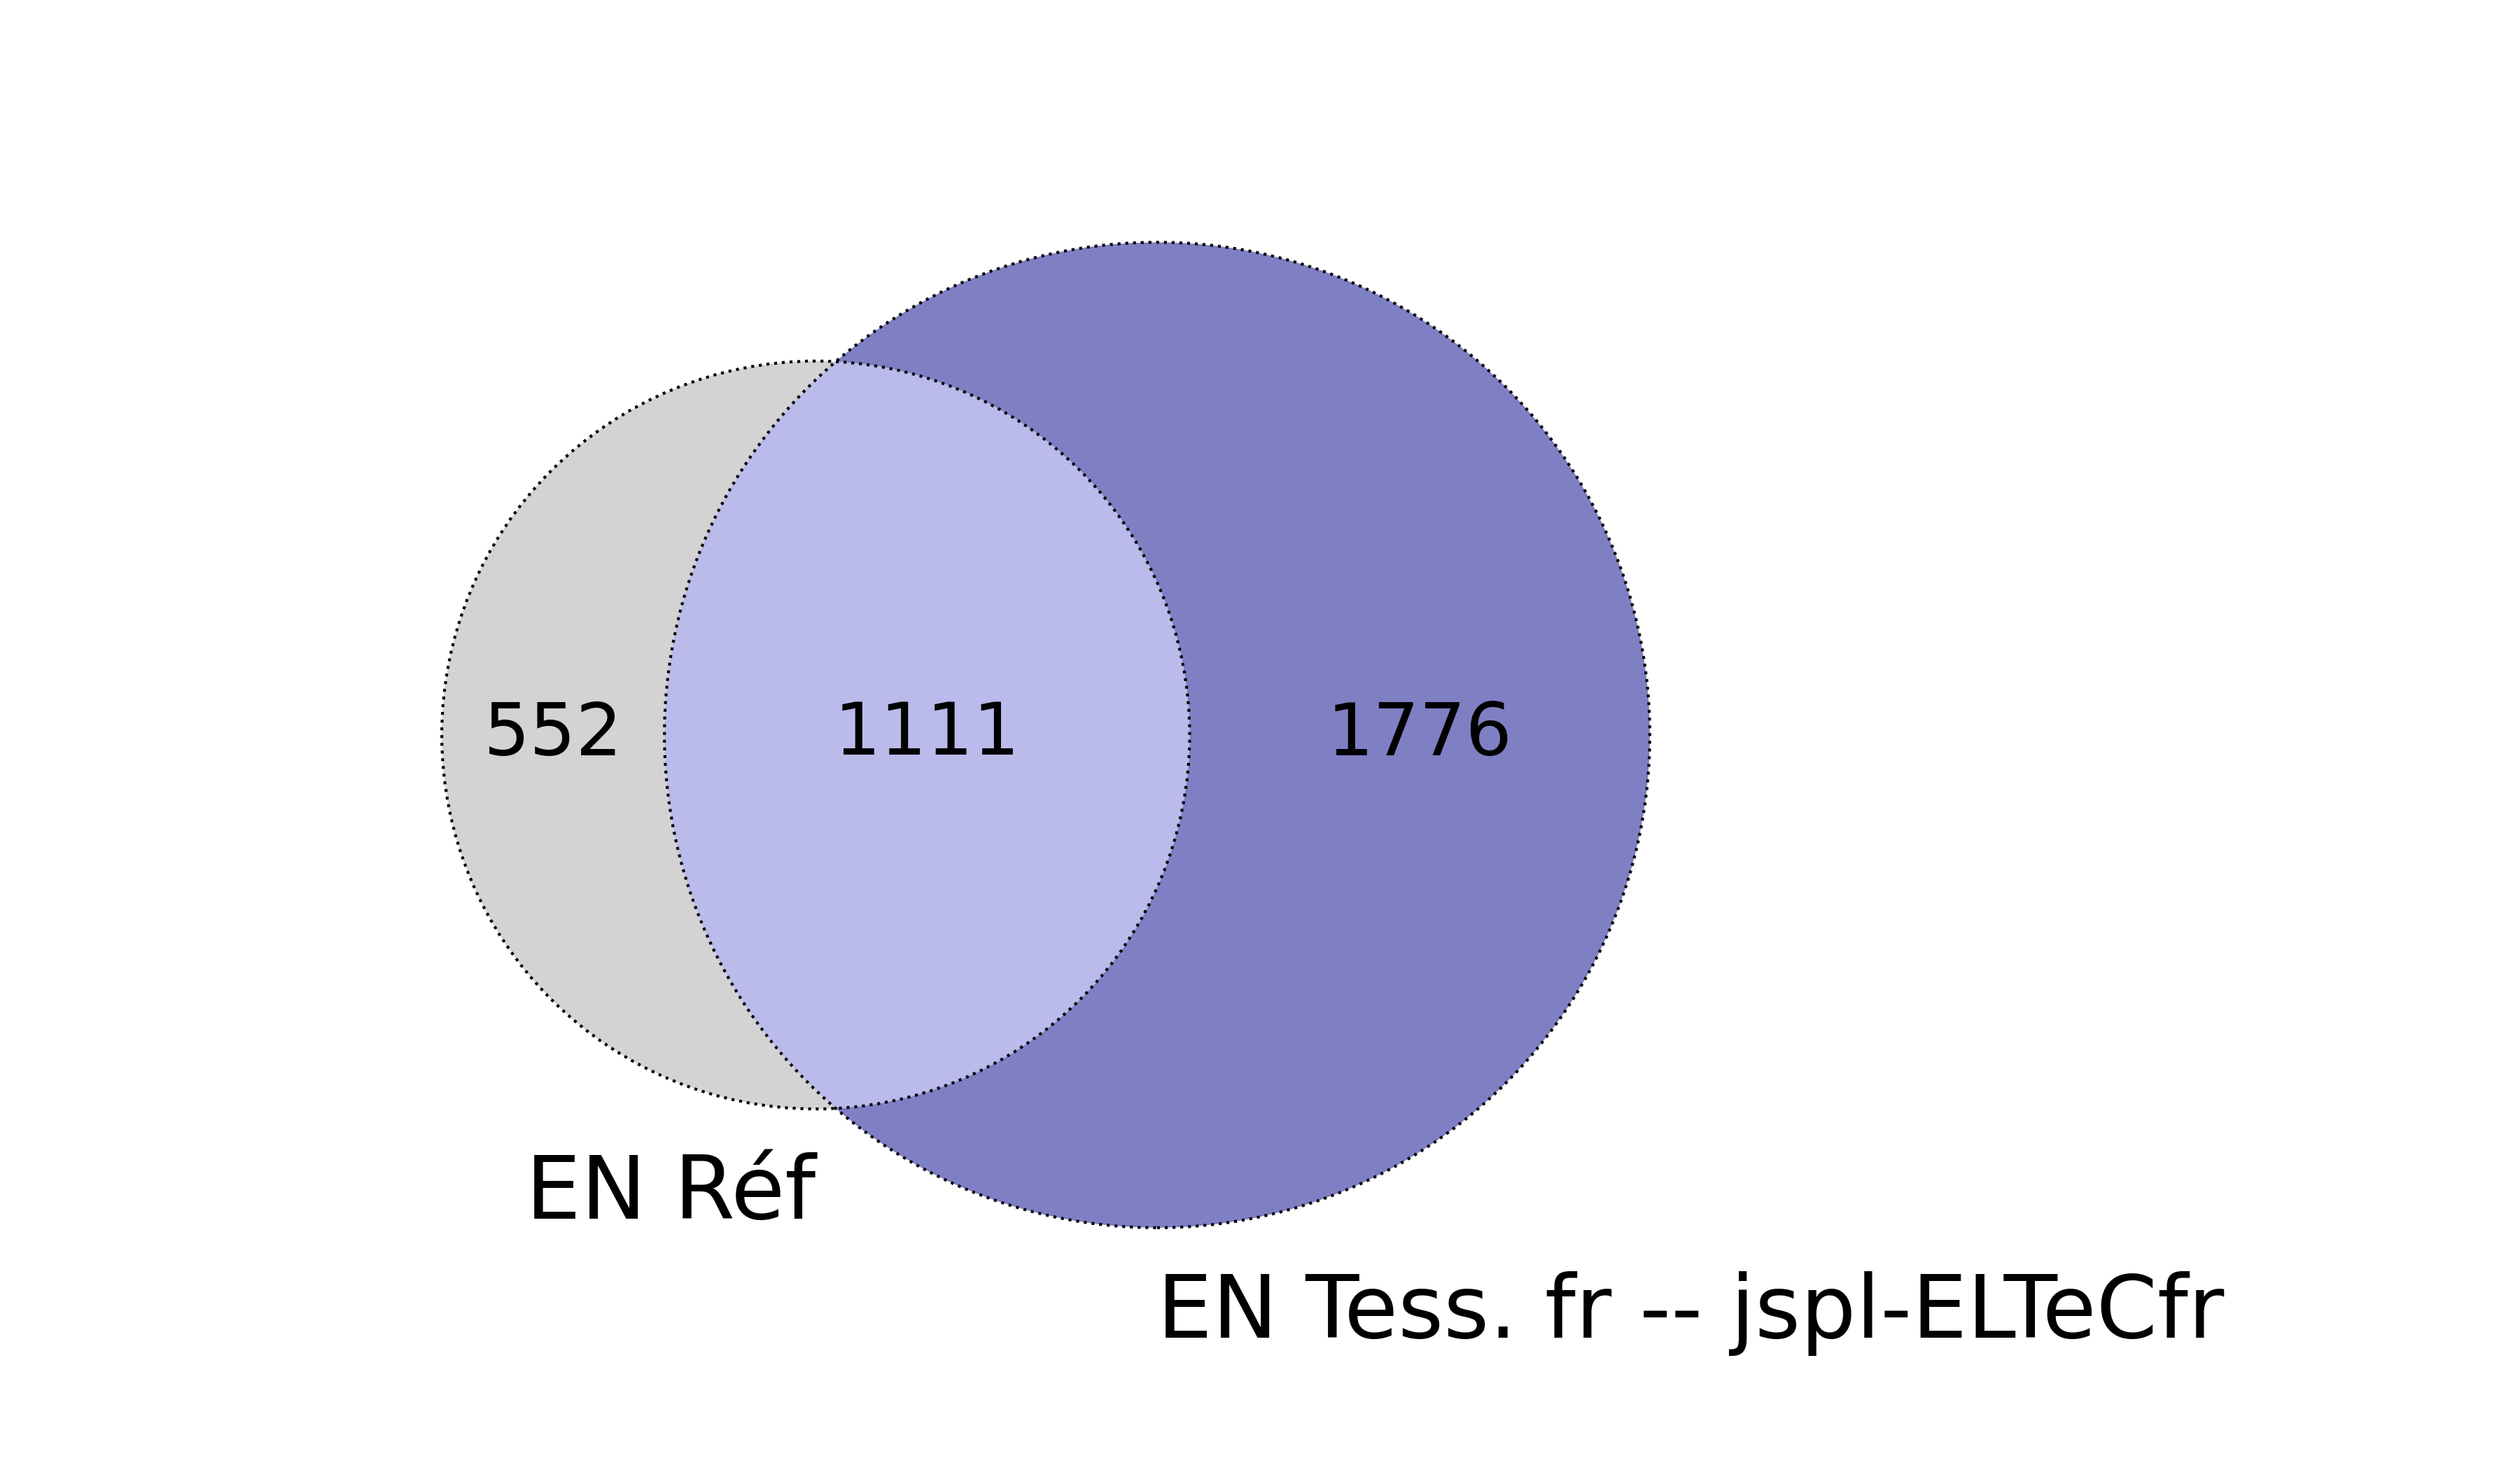
\includegraphics[width=1\textwidth]{IMAGES/INTERSECTIONS_GLOBALES/ELTeCFRA_Tess. fr -- jspl-ELTeCfr_stanza-concat_intersection.png}
%  \caption{Tess. fr. corrigé -- \texttt{stanza}}
%  \label{fig:ELTeCFRA_Tess. fr -- jspl-ELTeCfr_stanza-concat_intersection}
%  \end{subfigure}
%    \end{minipage}
%\begin{minipage}{7cm}
%  \begin{subfigure}{1\textwidth}
%  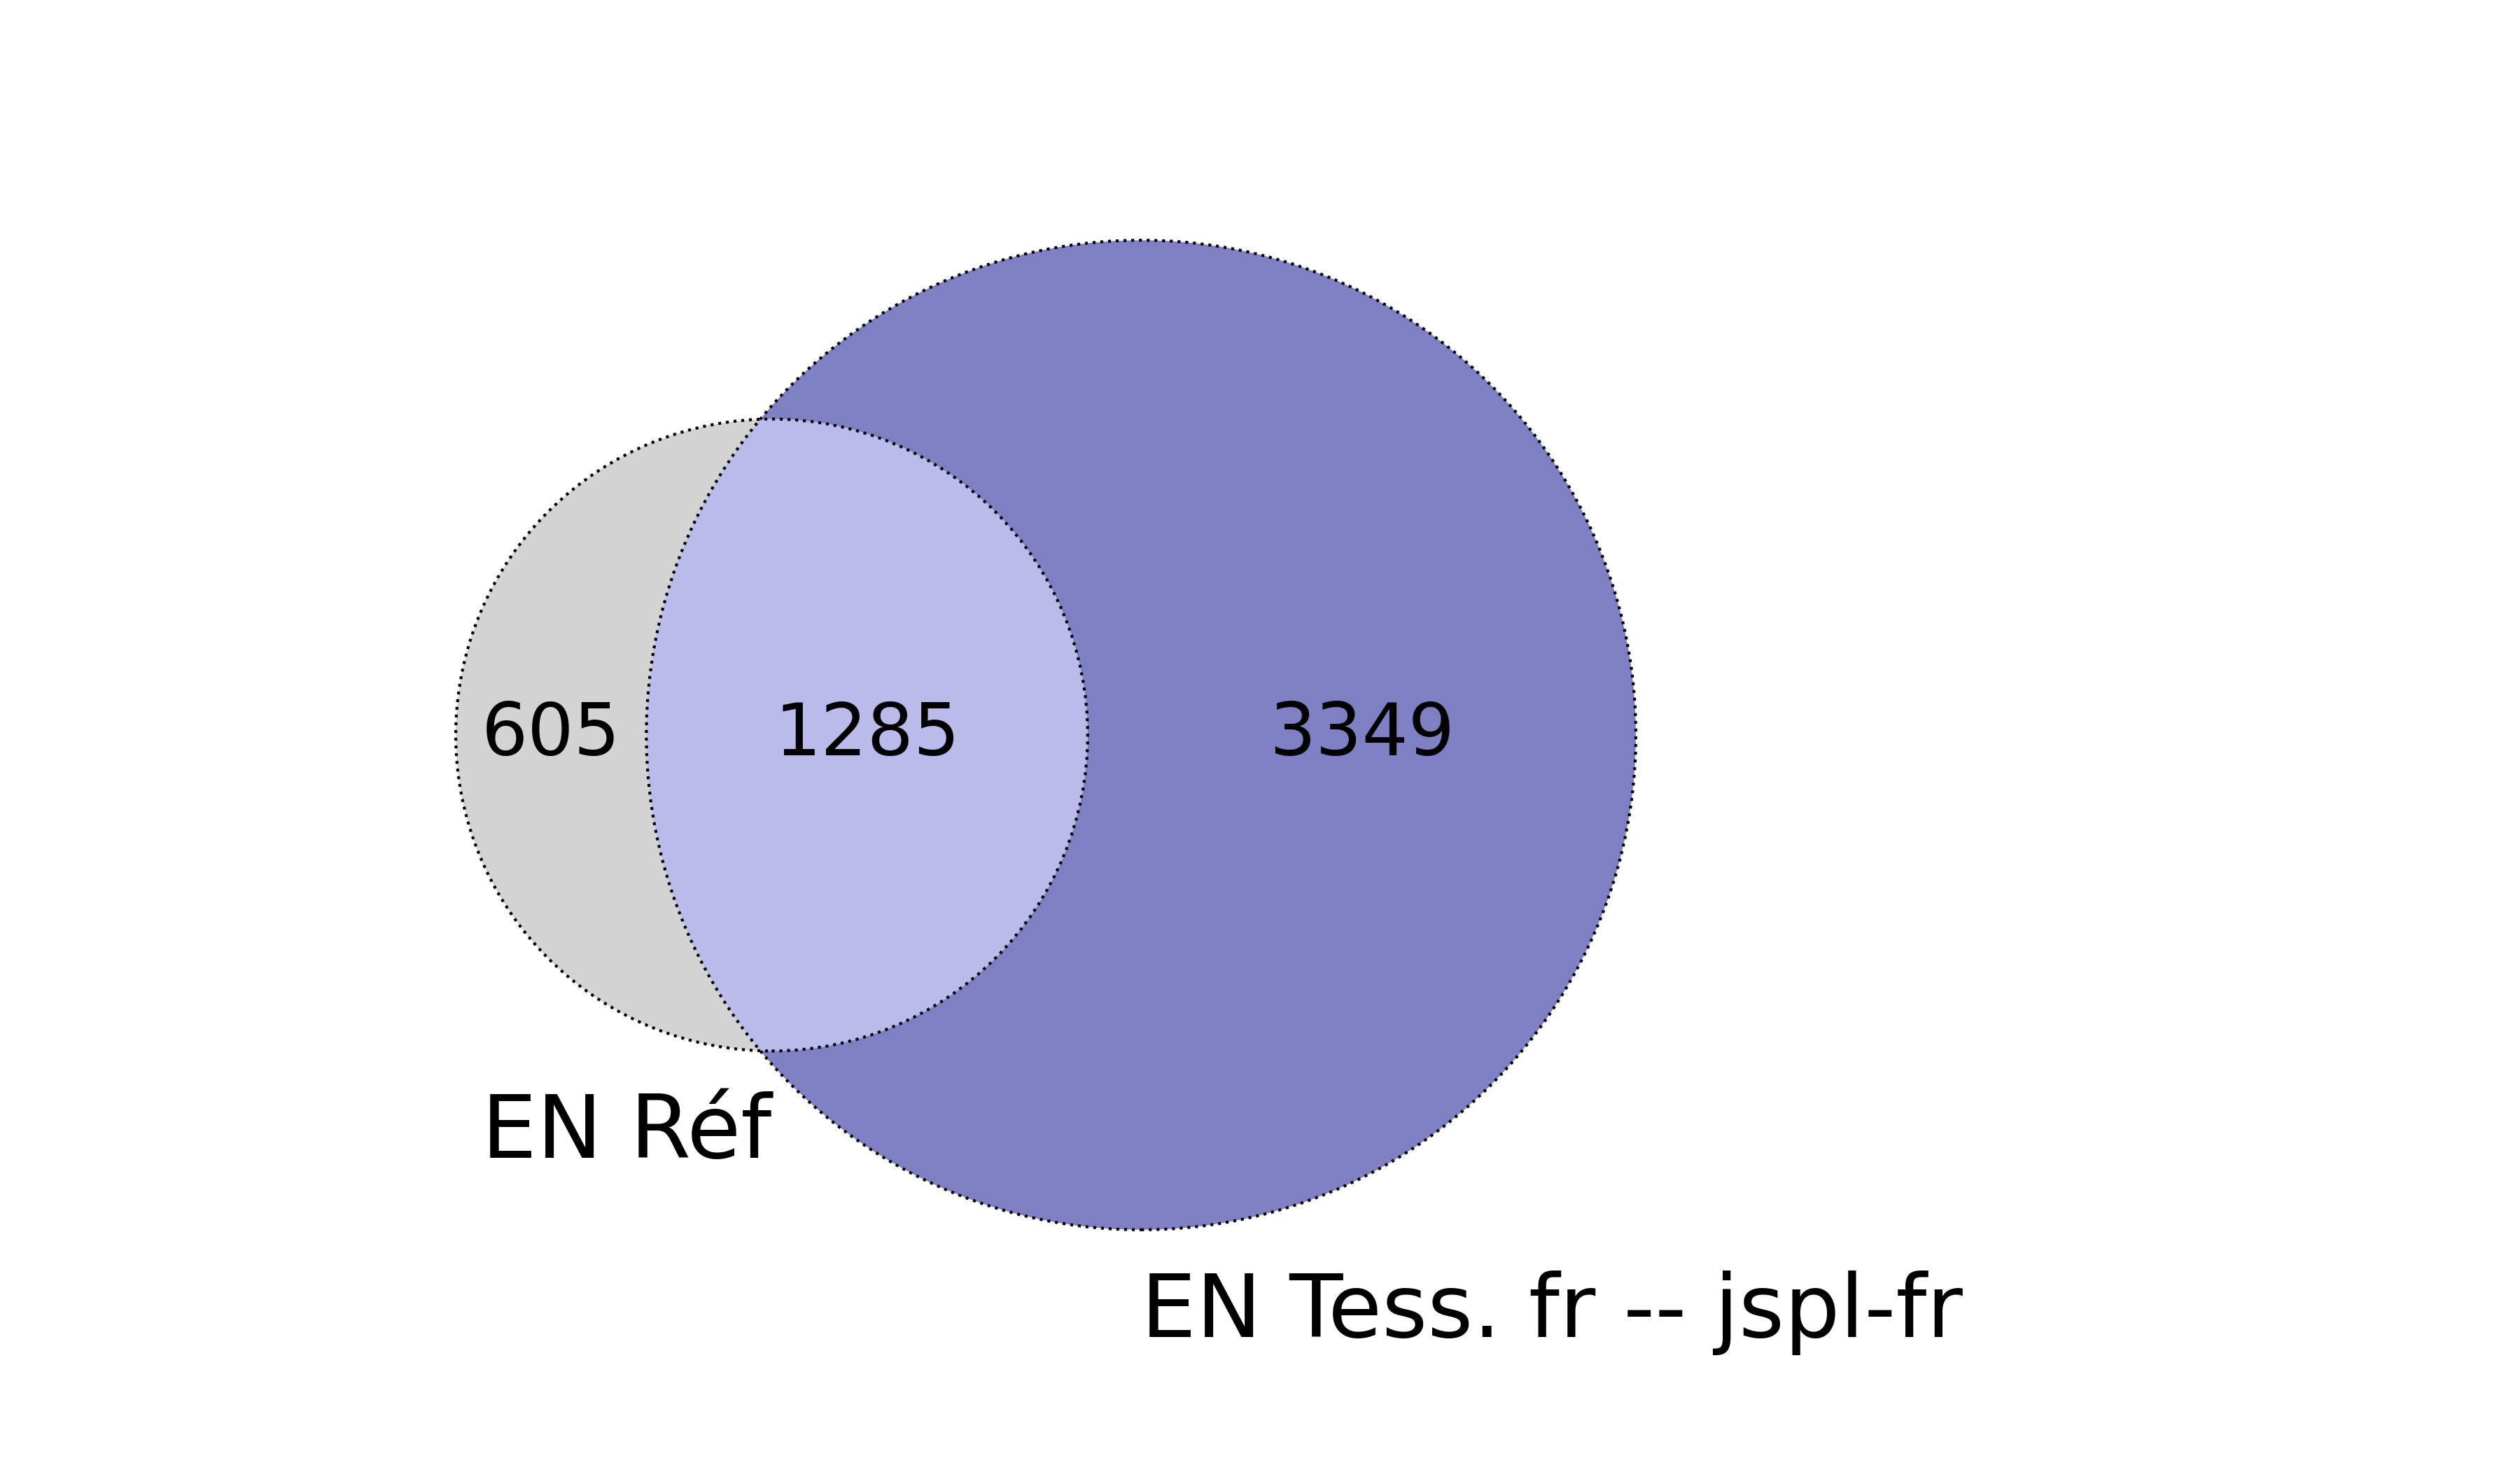
\includegraphics[width=1\textwidth]{IMAGES/INTERSECTIONS_GLOBALES/ELTeCFRA_Tess. fr -- jspl-fr_spacy-lg-concat_intersection.png} 
%  \caption{Tess. fr. corrigé -- \texttt{spaCy\_lg}}
%  \label{fig:ELTeCFRA_Tess. fr -- jspl-fr_spacy-lg-concat_intersection}
%  \end{subfigure}
%  \end{minipage}
%  \begin{minipage}{7cm}
%  \begin{subfigure}{1\textwidth}
%  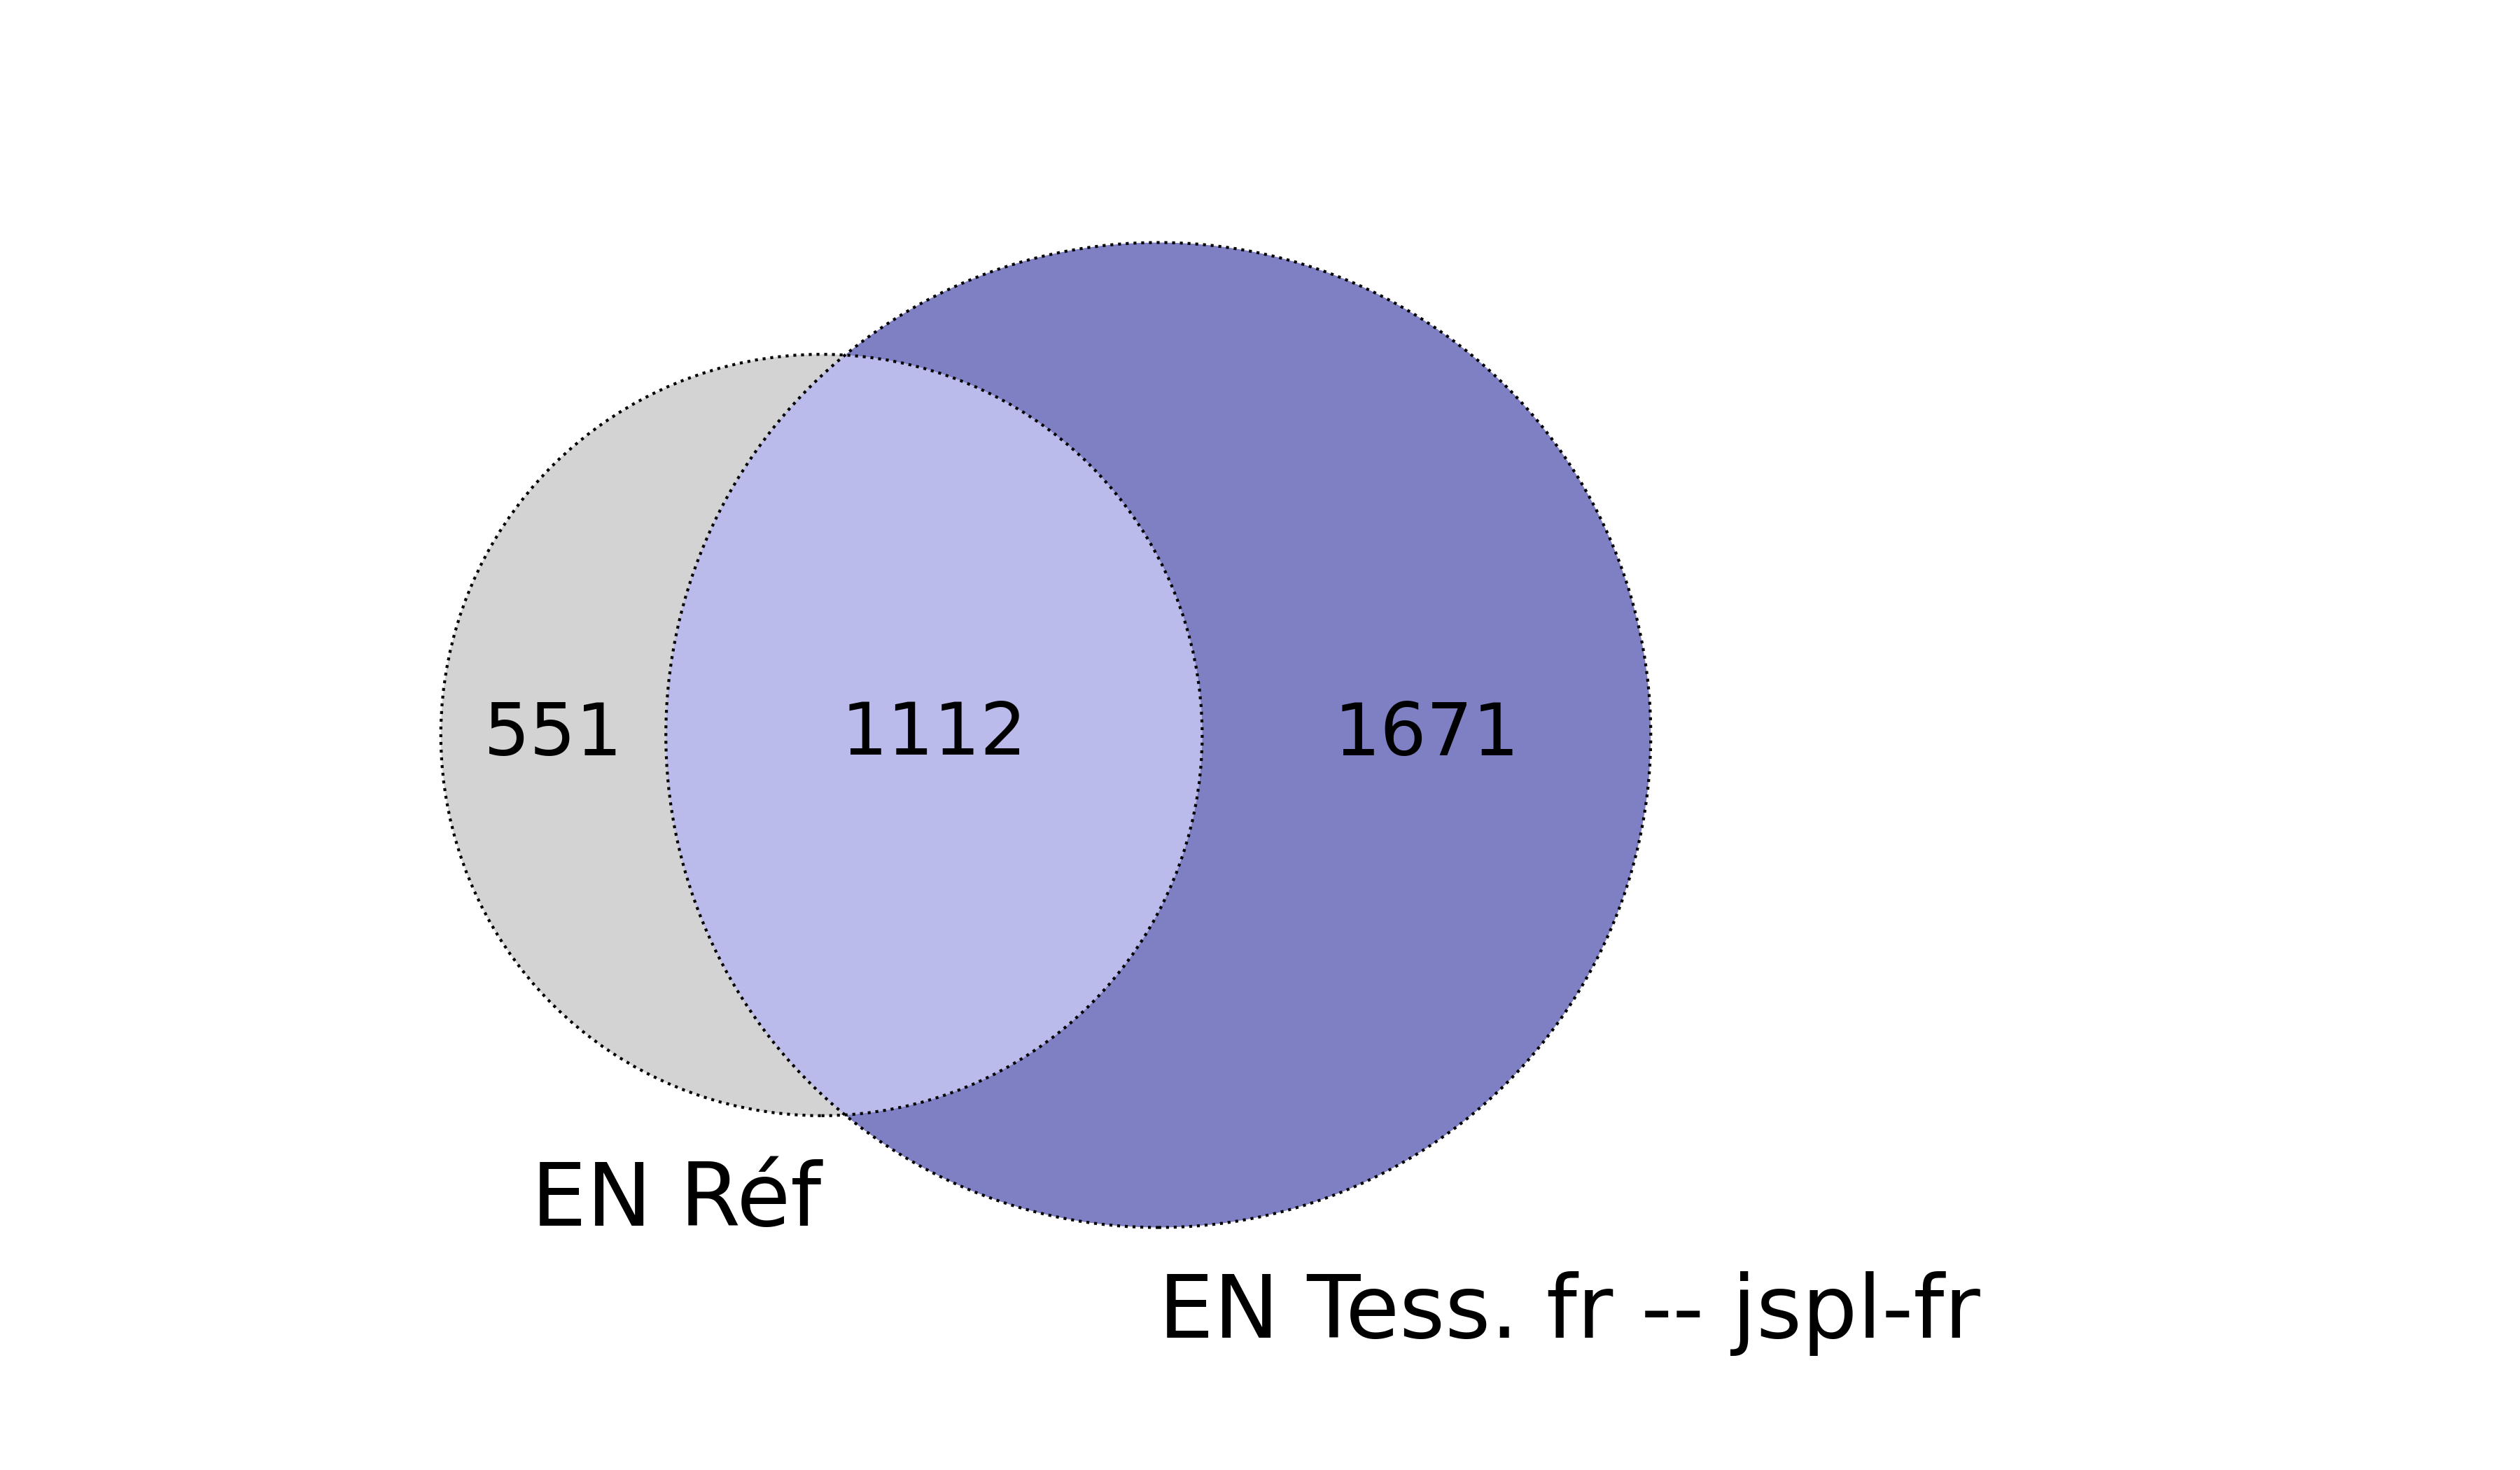
\includegraphics[width=1\textwidth]{IMAGES/INTERSECTIONS_GLOBALES/ELTeCFRA_Tess. fr -- jspl-fr_stanza-concat_intersection.png}
%  \caption{Tess. fr. corrigé -- \texttt{stanza}}
%  \label{fig:ELTeCFRA_Tess. fr -- jspl-fr_stanza-concat_intersection}
%  \end{subfigure}
%    \end{minipage}
%\caption{Intersections pour la configuration Tess-\texttt{spaCy\_lg} corrigées avec le modèle pré-entrainer de JamSpell et le modèle ELTeC, pour le corpus ELTeC français.}
%\label{fig:intersection-globale-tess}
%\end{figure}
\subsection{Comment dépasser les problèmes d'alignements ? }
\label{subsec:ditances_creux_COR-OCR-IMPACT-NER}
\subsubsection{Mesures de distance textuelle}

Dans le but d'approfondir nos évaluations et de dépasser les verrous de l'évaluation stricte, nous employons des mesures de distance textuelle afin de rendre plus souple nos critères d'évaluation des résultats de la REN sur les sorties de ROC bruitées et leurs corrections automatiques. Nous avons privilégié les métriques de Jaccard\footnote{Nous présentons uniquement des résultats pour cosinus ; pour les résultats Jaccard, \textit{cf.} le dépôt GitHub : \url{https://github.com/anonymous}} et cosinus, calculées sur les bigrammes et trigrammes de caractères\footnote{Nous avons vectorisé le texte avec la librairie \texttt{CountVectorizer} pour les deux distances.}, car elles sont considérées comme des mesures de référence quand il est question de (dis)similarité textuelle \cite{buscaldi2020calcul}. 

\begin{figure}[h!]
   \centering
      \begin{subfigure}{0.45\textwidth}
  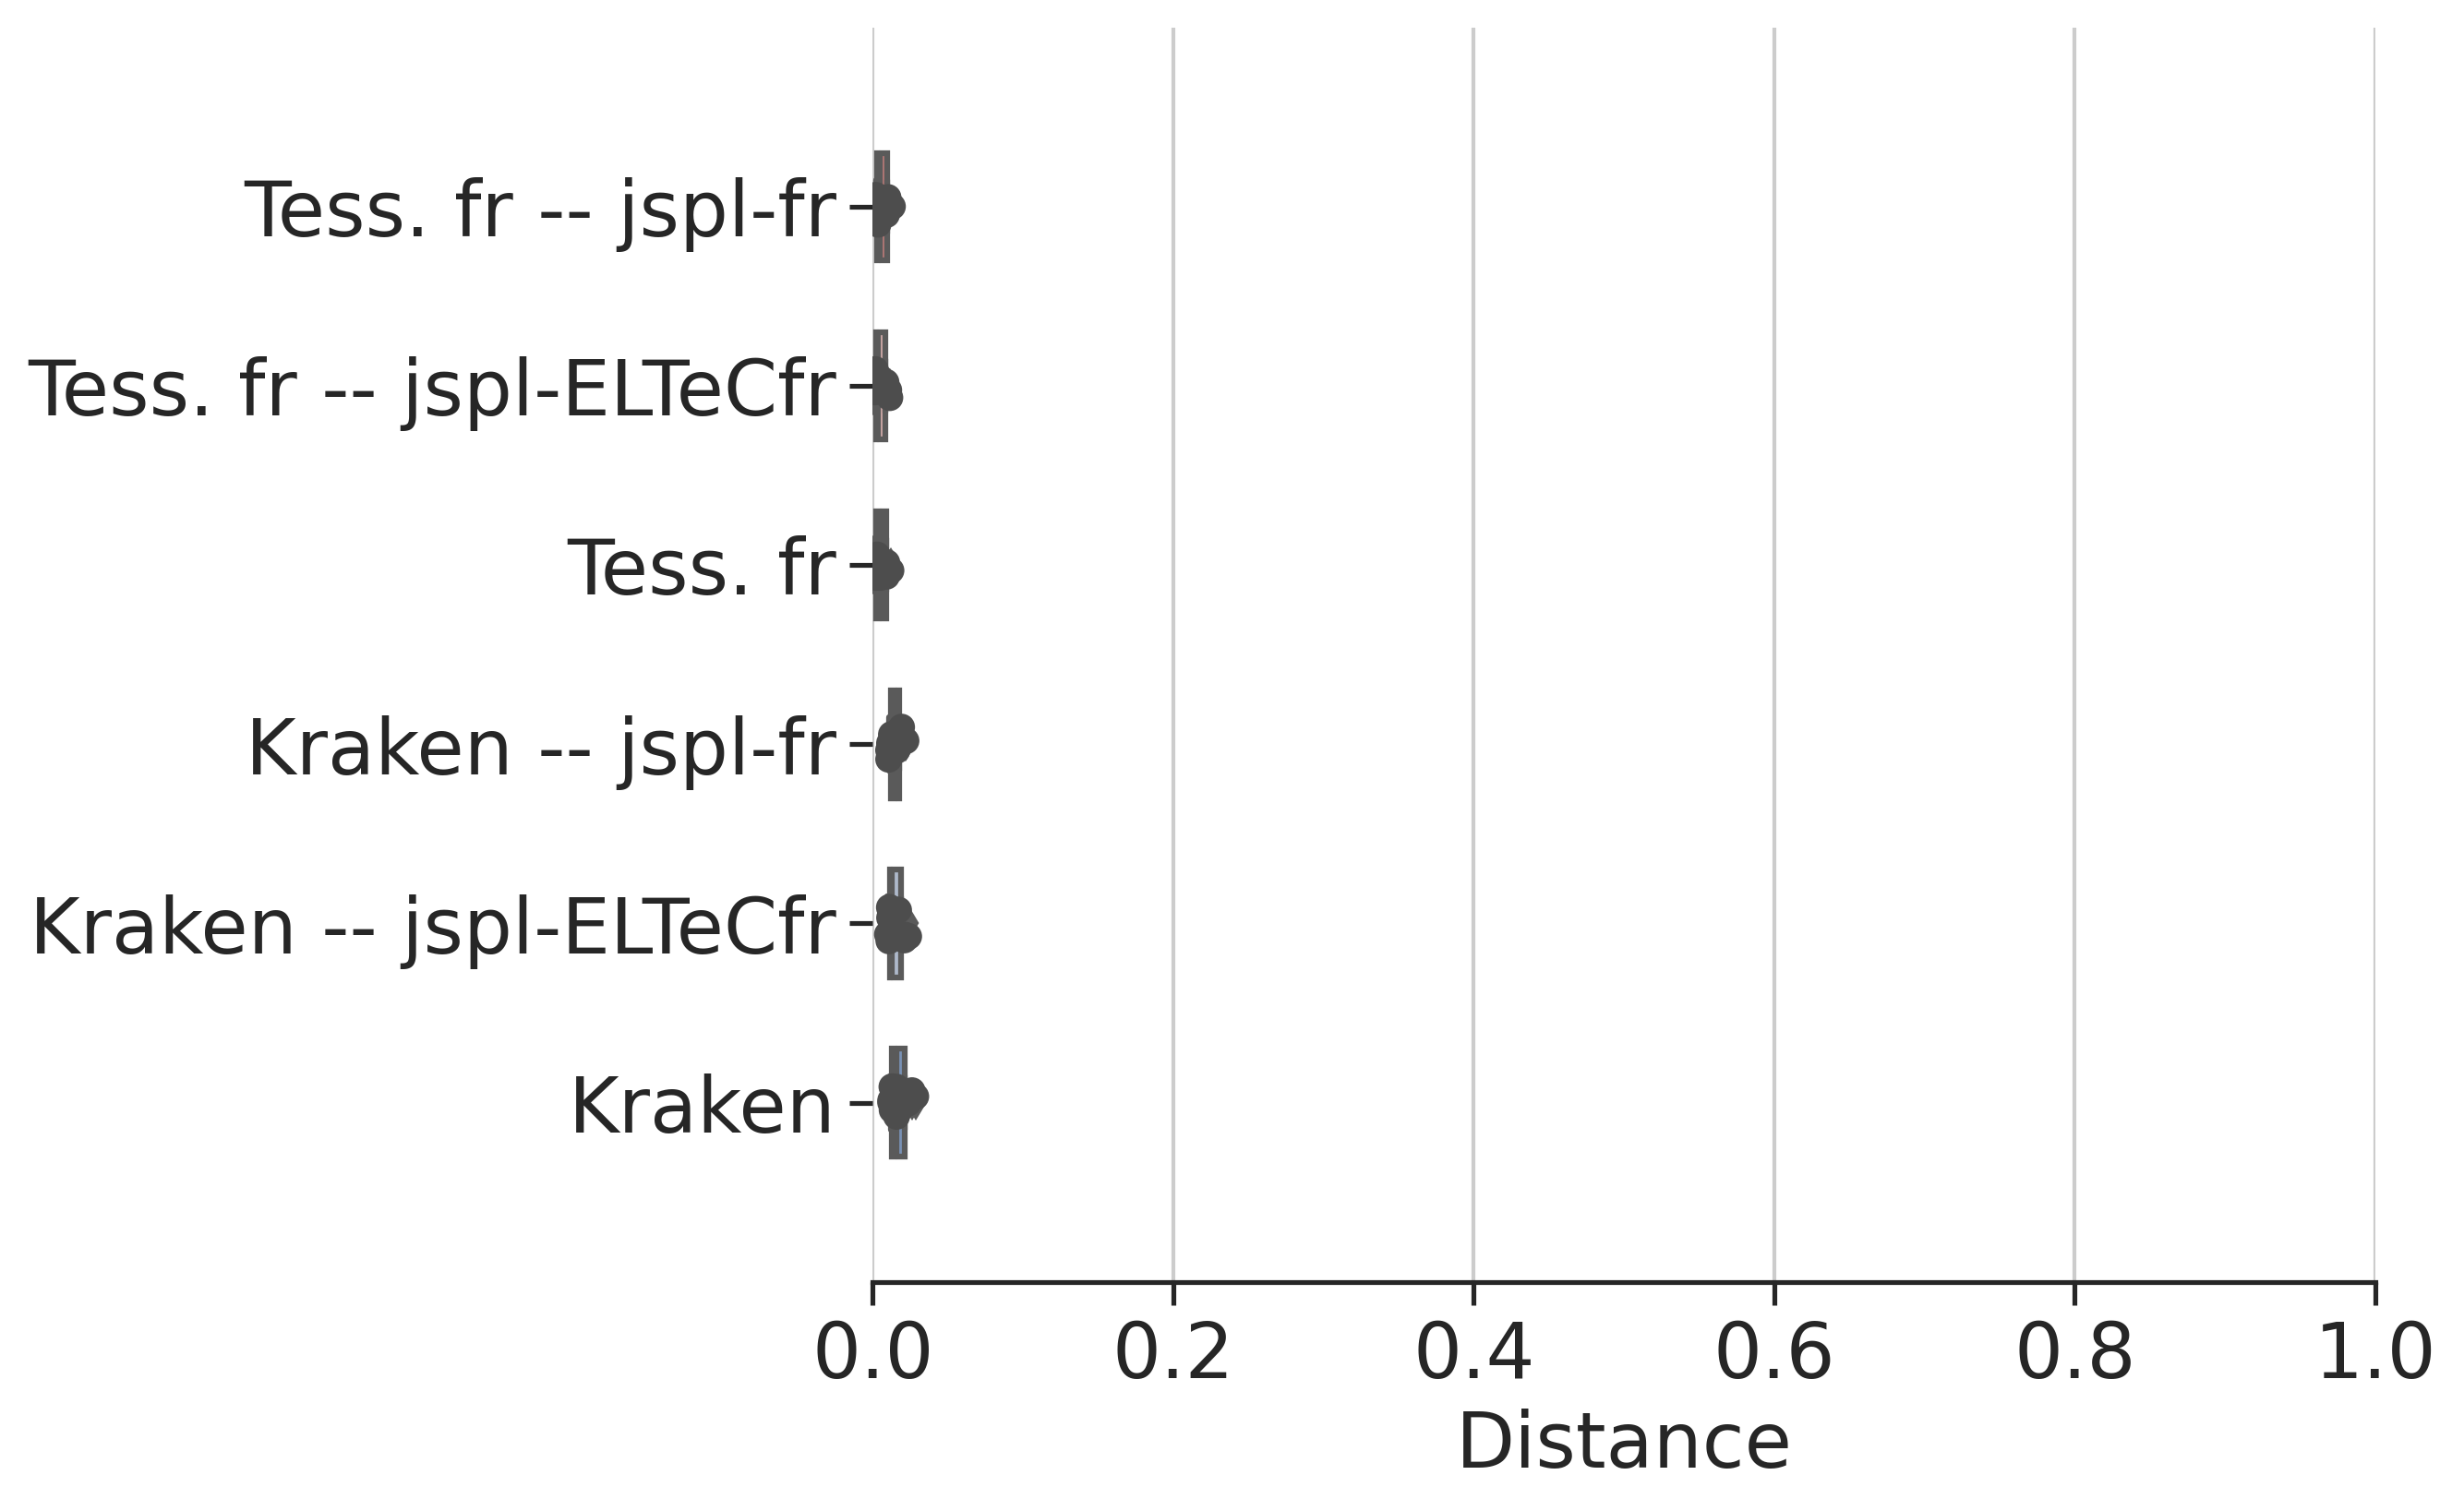
\includegraphics[height=.65\textwidth]{IMAGES/Boite-moustache/ELTeC-Fra_REF_cosinus.png} 
        \caption{ELTeC-Fra cosinus}
        \label{fig:ELTeC-Fra_REF_cosinus}
   \end{subfigure}
       \begin{subfigure}{0.5\textwidth}
  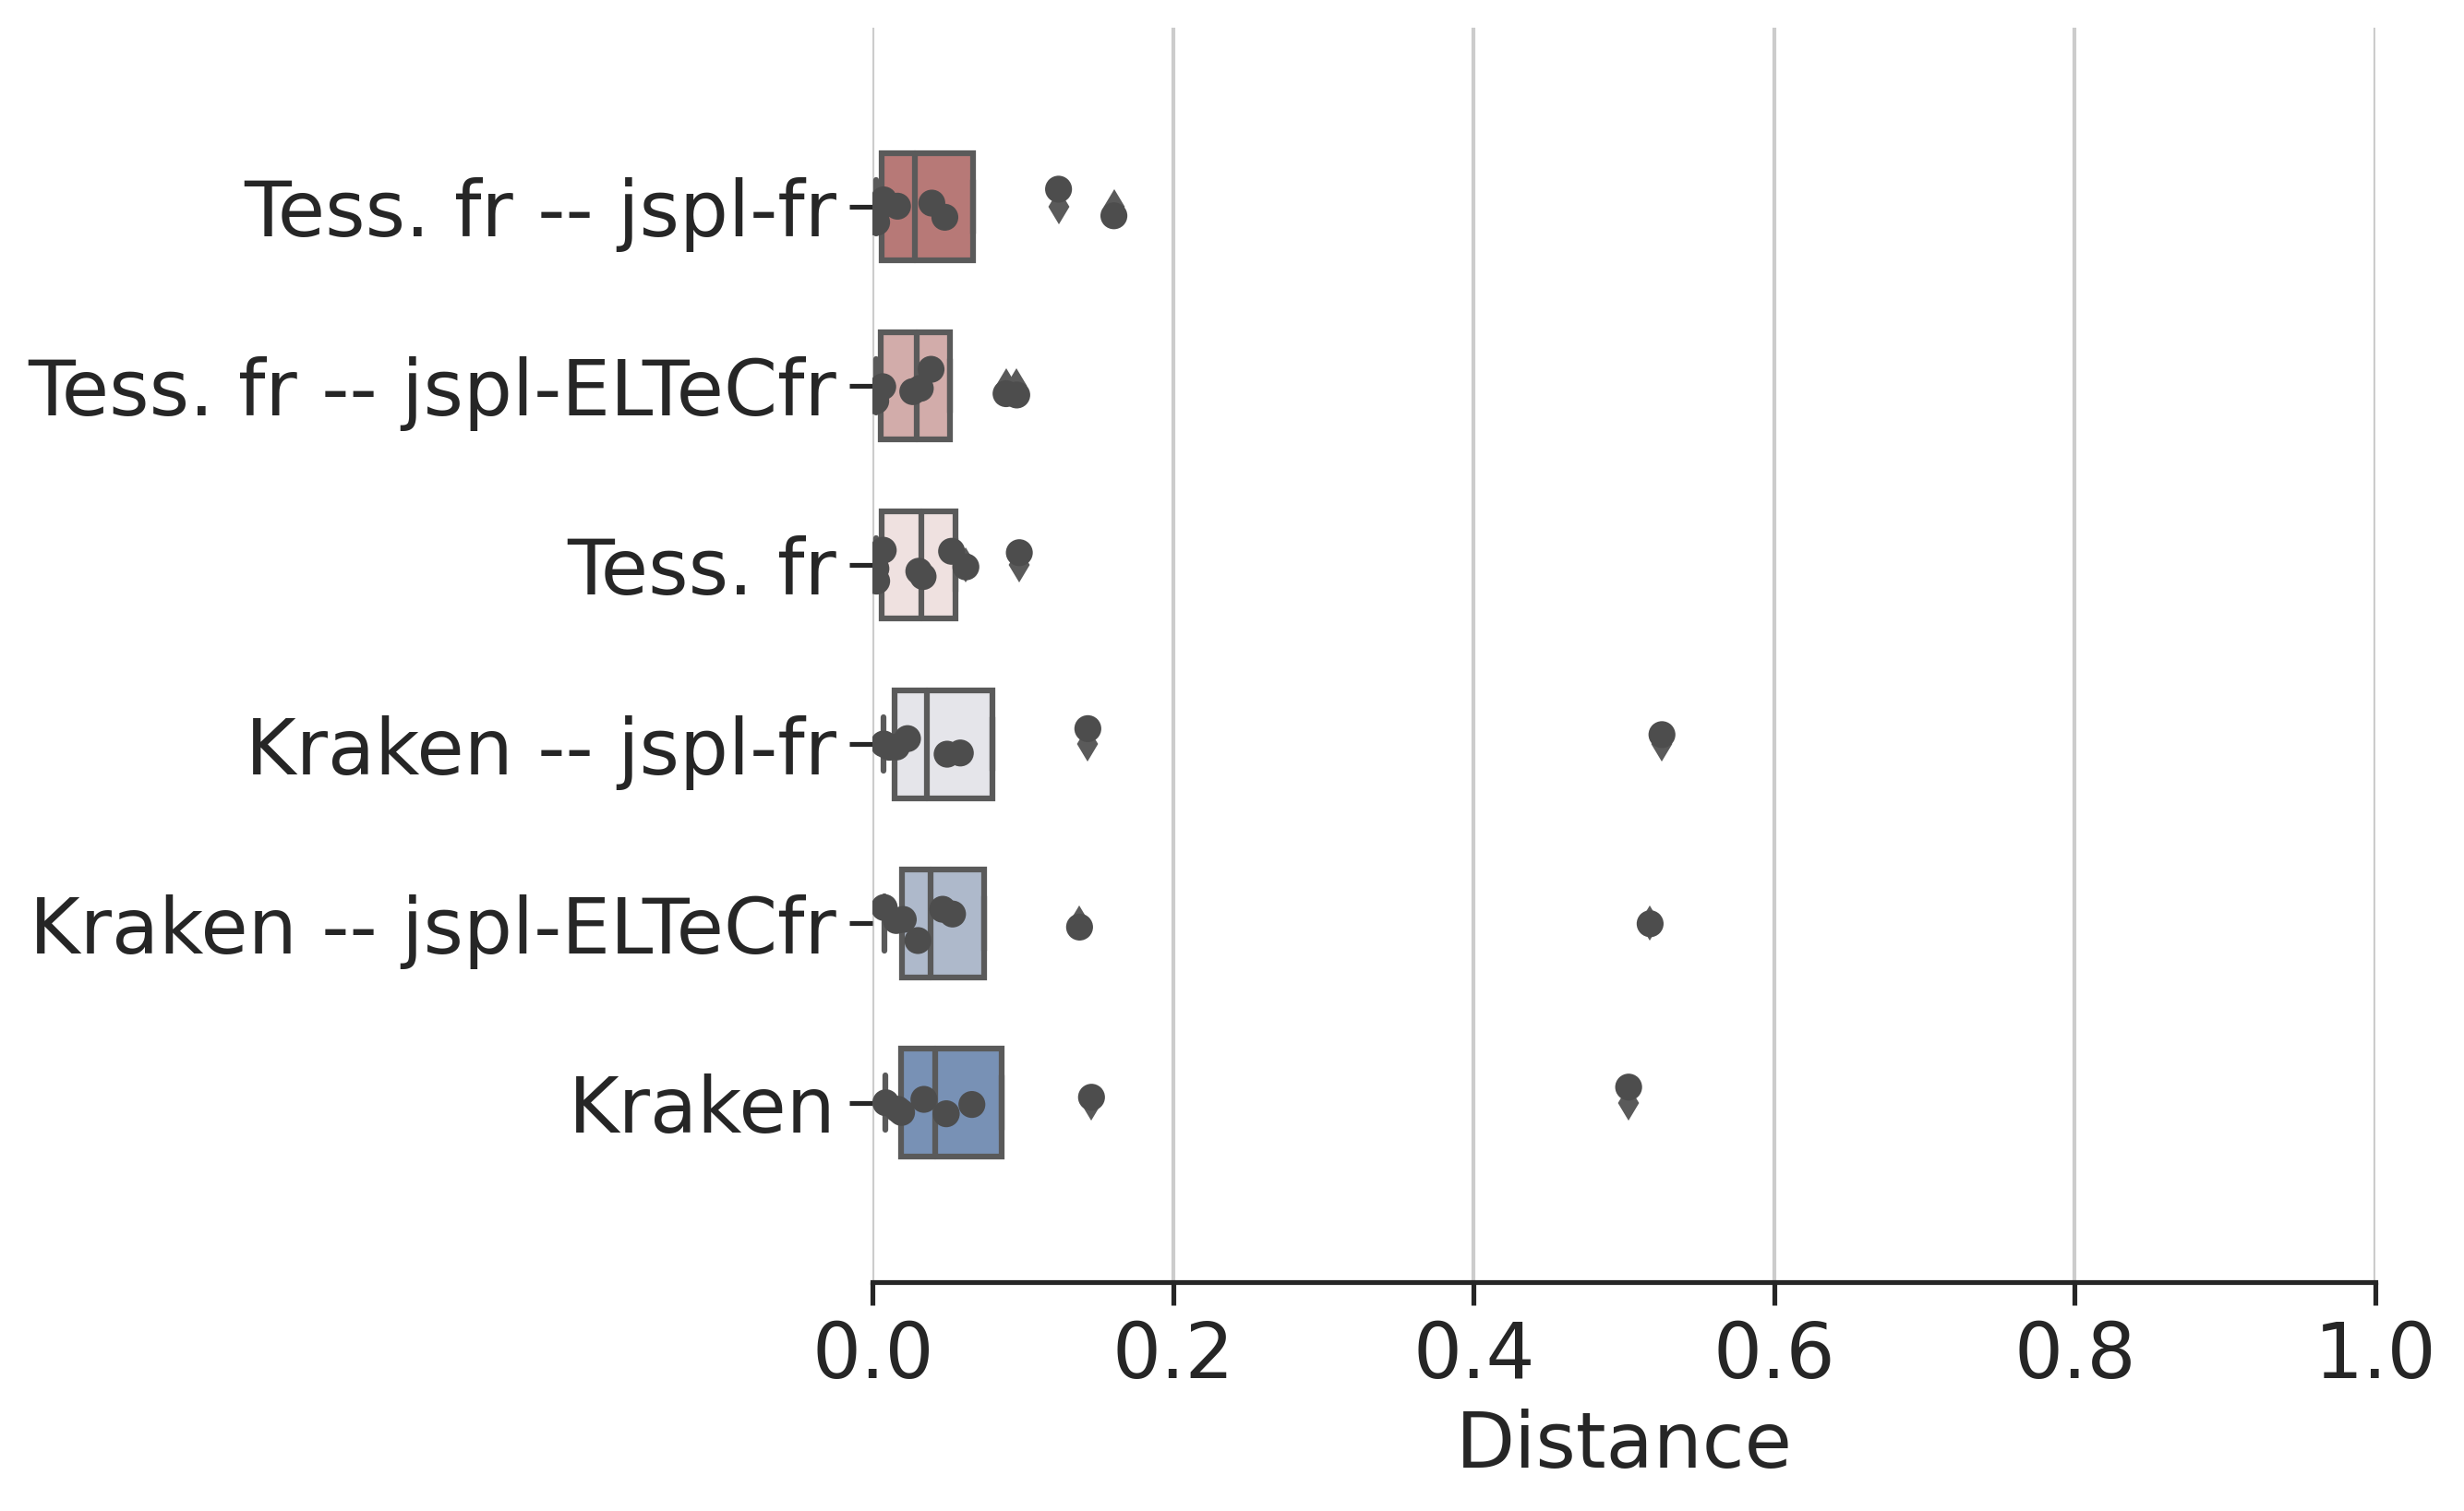
\includegraphics[height=.65\textwidth]{IMAGES/Boite-moustache/TGB_REF_cosinus.png} 
        \caption{TGB cosinus}
   \end{subfigure}
   
    \begin{subfigure}{0.5\textwidth}
  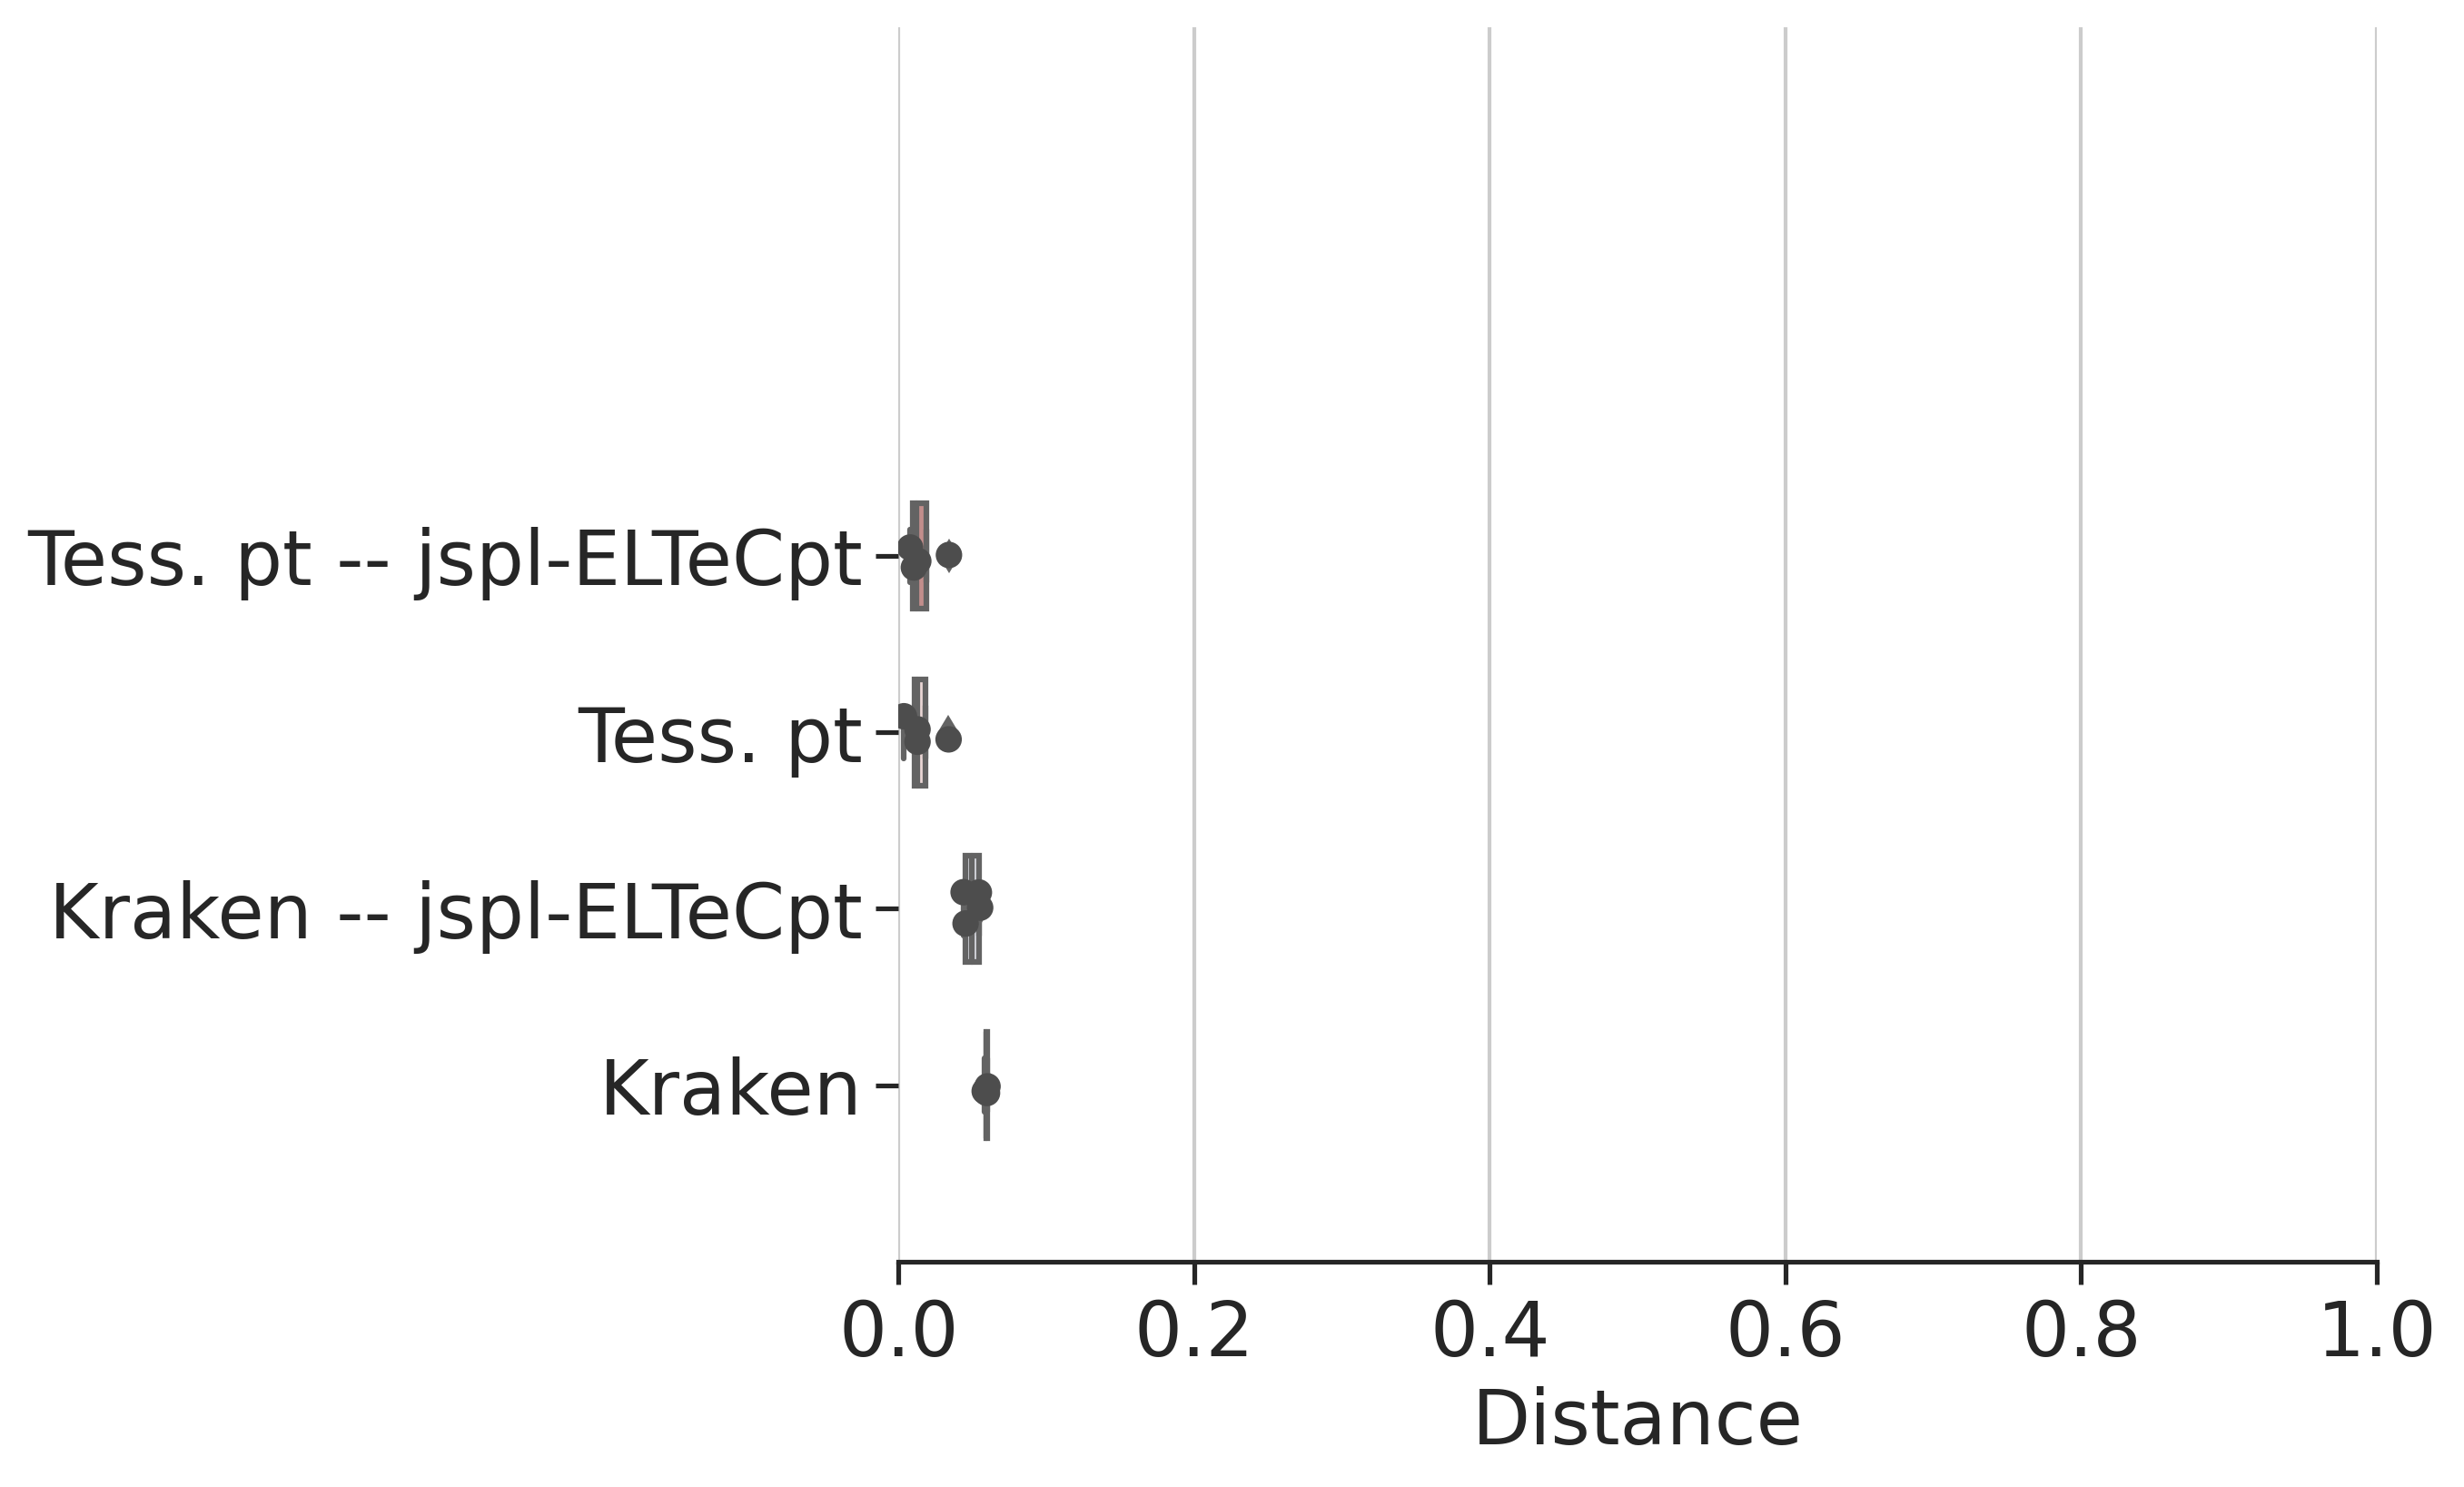
\includegraphics[height=.65\textwidth]{IMAGES/Boite-moustache/ELTeC-Por_REF_cosinus.png} 
        \caption{ELTeC-Por cosinus}
        \label{fig:ELTeC-Por_REF_cosinus}
   \end{subfigure}   
         \begin{subfigure}{0.45\textwidth}
  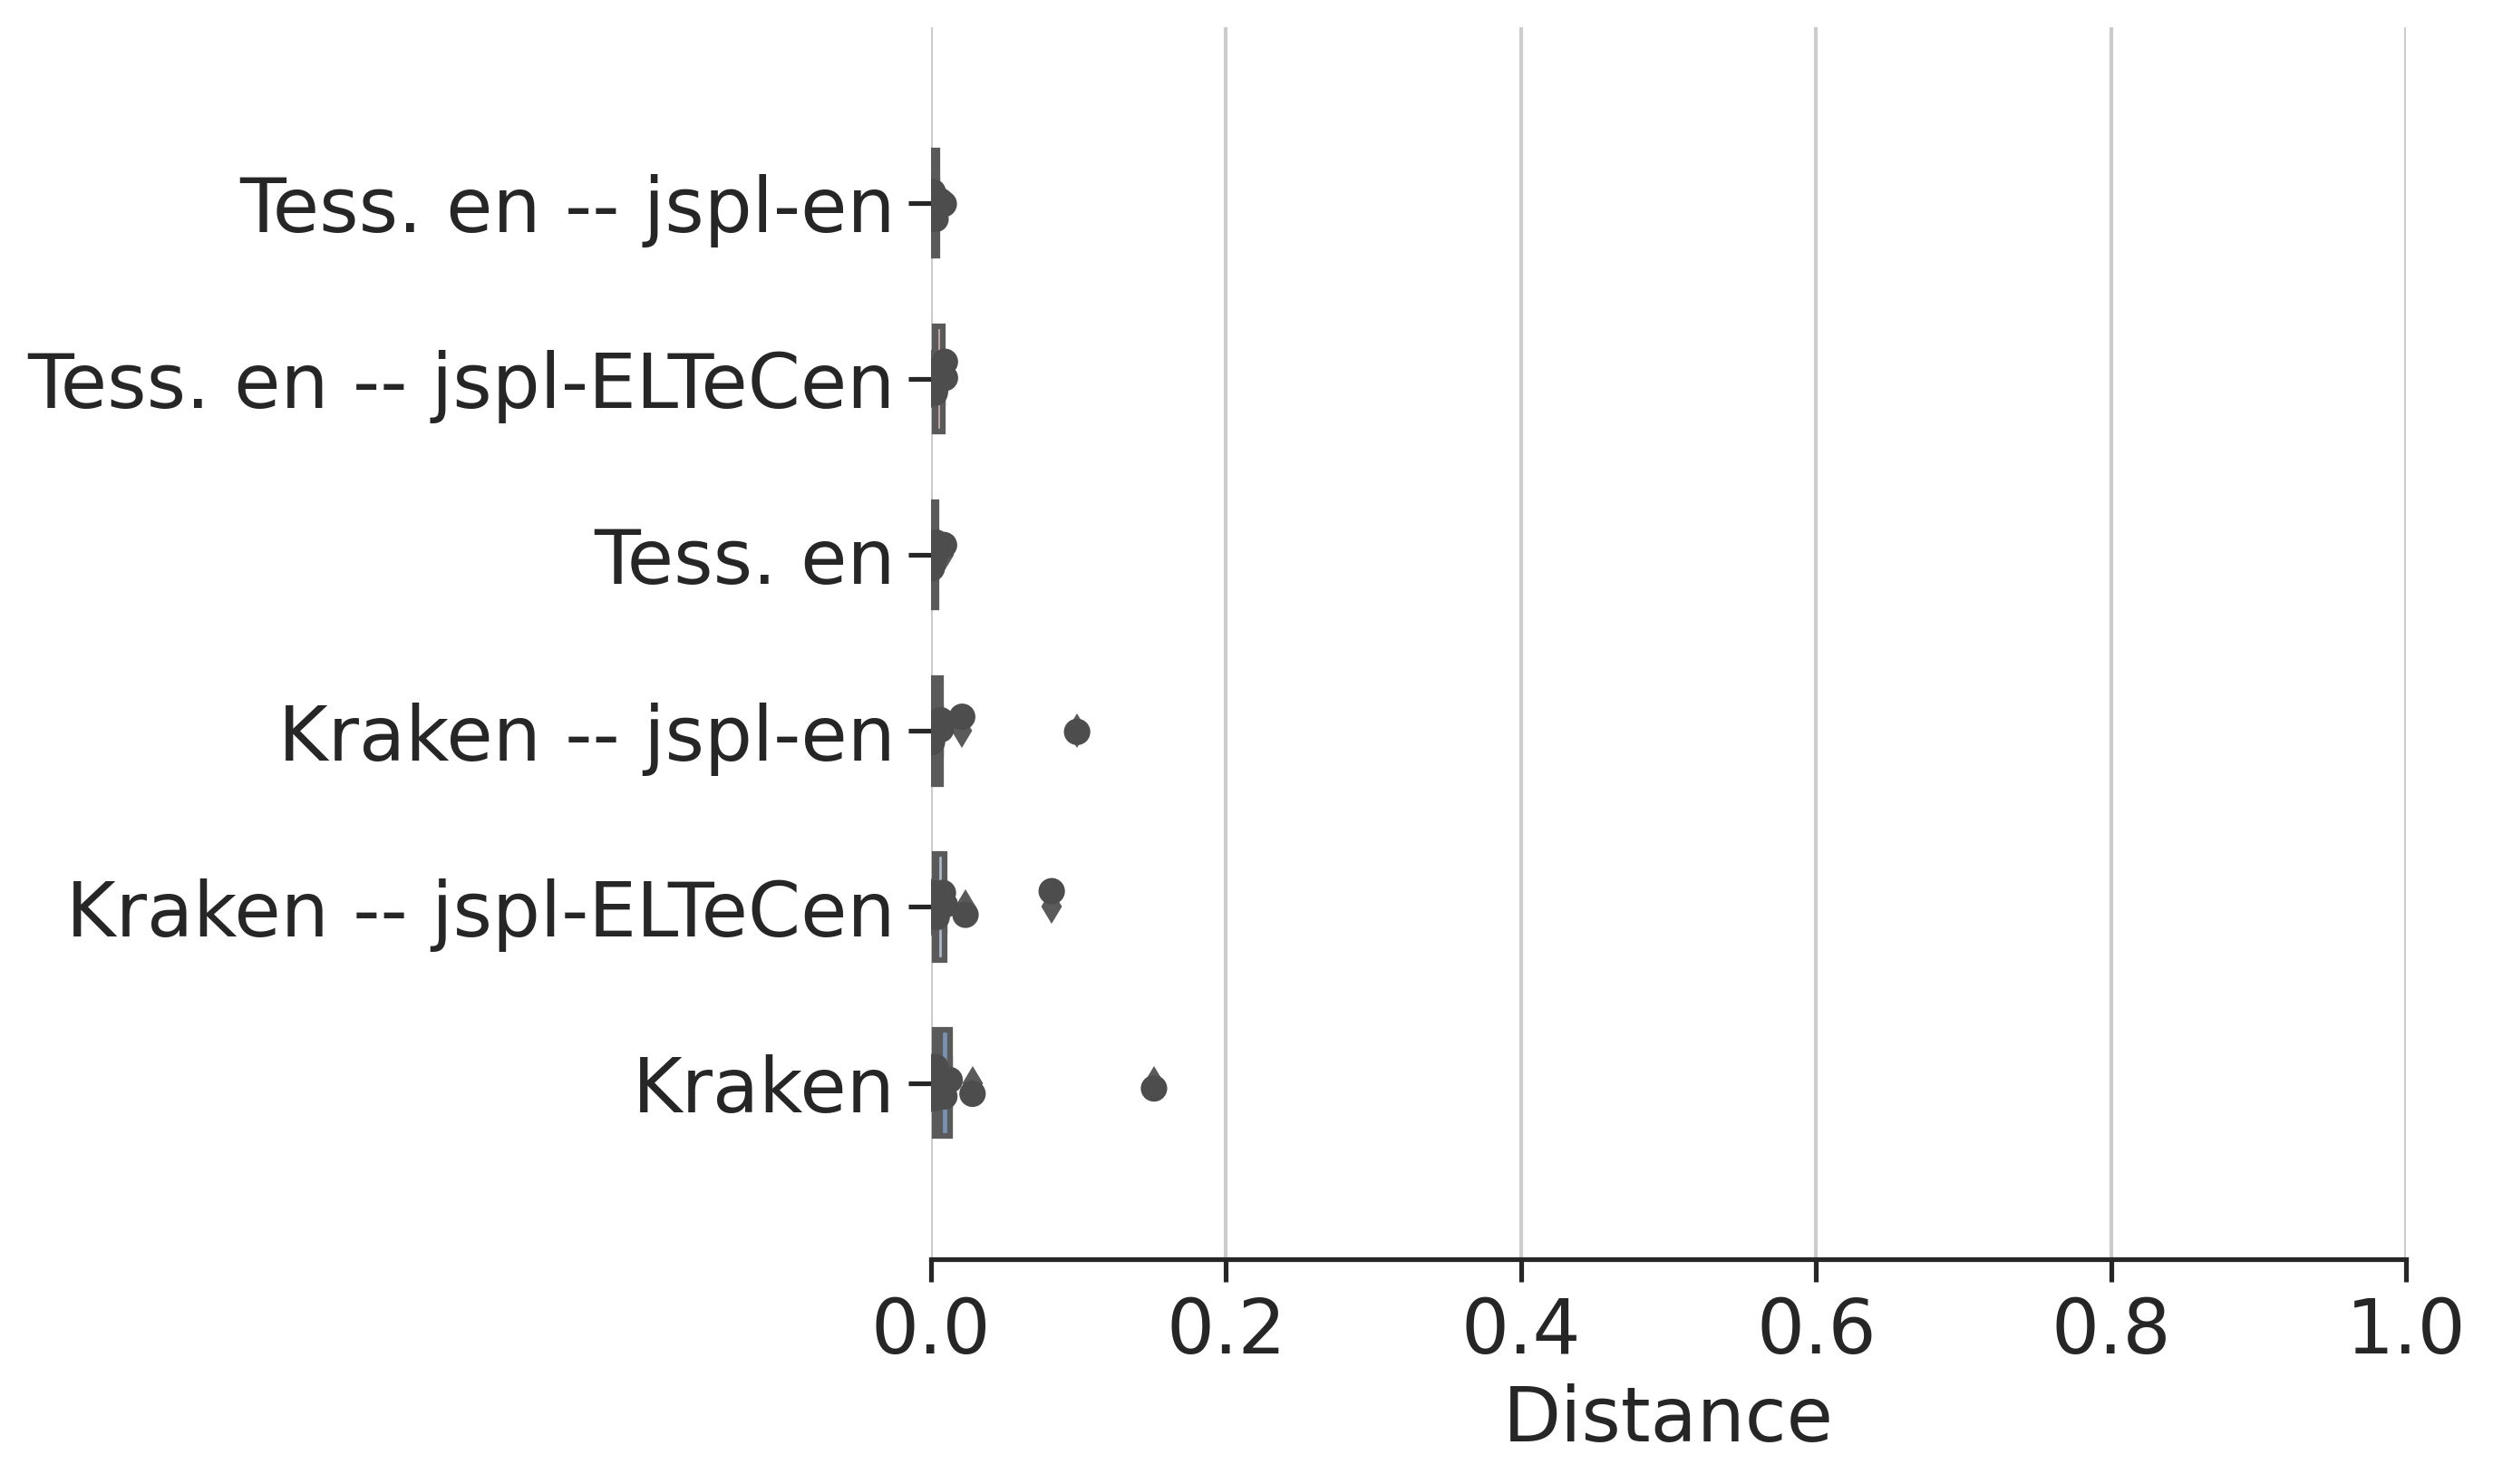
\includegraphics[height=.65\textwidth]{IMAGES/Boite-moustache/ELTeC-Eng_REF_cosinus.png} 
        \caption{ELTeC-Eng cosinus.png}
   \end{subfigure}   
    \caption{Distances calculées entre les textes de référence et les versions de ROC.}
    \label{fig:distances_ref_roc}
\end{figure}

Pour lire les figures \ref{fig:distances_ref_roc} et \ref{fig:Cosinus-spacy-lg}, il faut noter que plus la boîte est proche de zéro, plus les sorties comparées sont similaires. La figure \ref{fig:distances_ref_roc} illustre les résultats obtenus pour les textes de réf. et les différentes versions de ROC pour tous les corpus avec une distance cosinus. La figure \ref{fig:Cosinus-spacy-lg} montre les résultats en comparant les sorties de REN obtenues sur les textes de réf. et celles des différentes configurations évaluées (tableau \ref{tab:config}). 
Après une observation des différentes mesures de distance présentées pour chaque corpus évalué, on note l'écart constant et considérable entre les résultats de Jaccard et cosinus. Les résutats pour Jaccard sont souvent proches de 1, tandis que ceux de cosinus sont proches de 0 pour les mêmes configurations. Il semble que les métriques cosinus et Jaccard ne mesurent pas la même chose. 

\begin{figure}[h!]

    \begin{subfigure}{0.45\textwidth}
  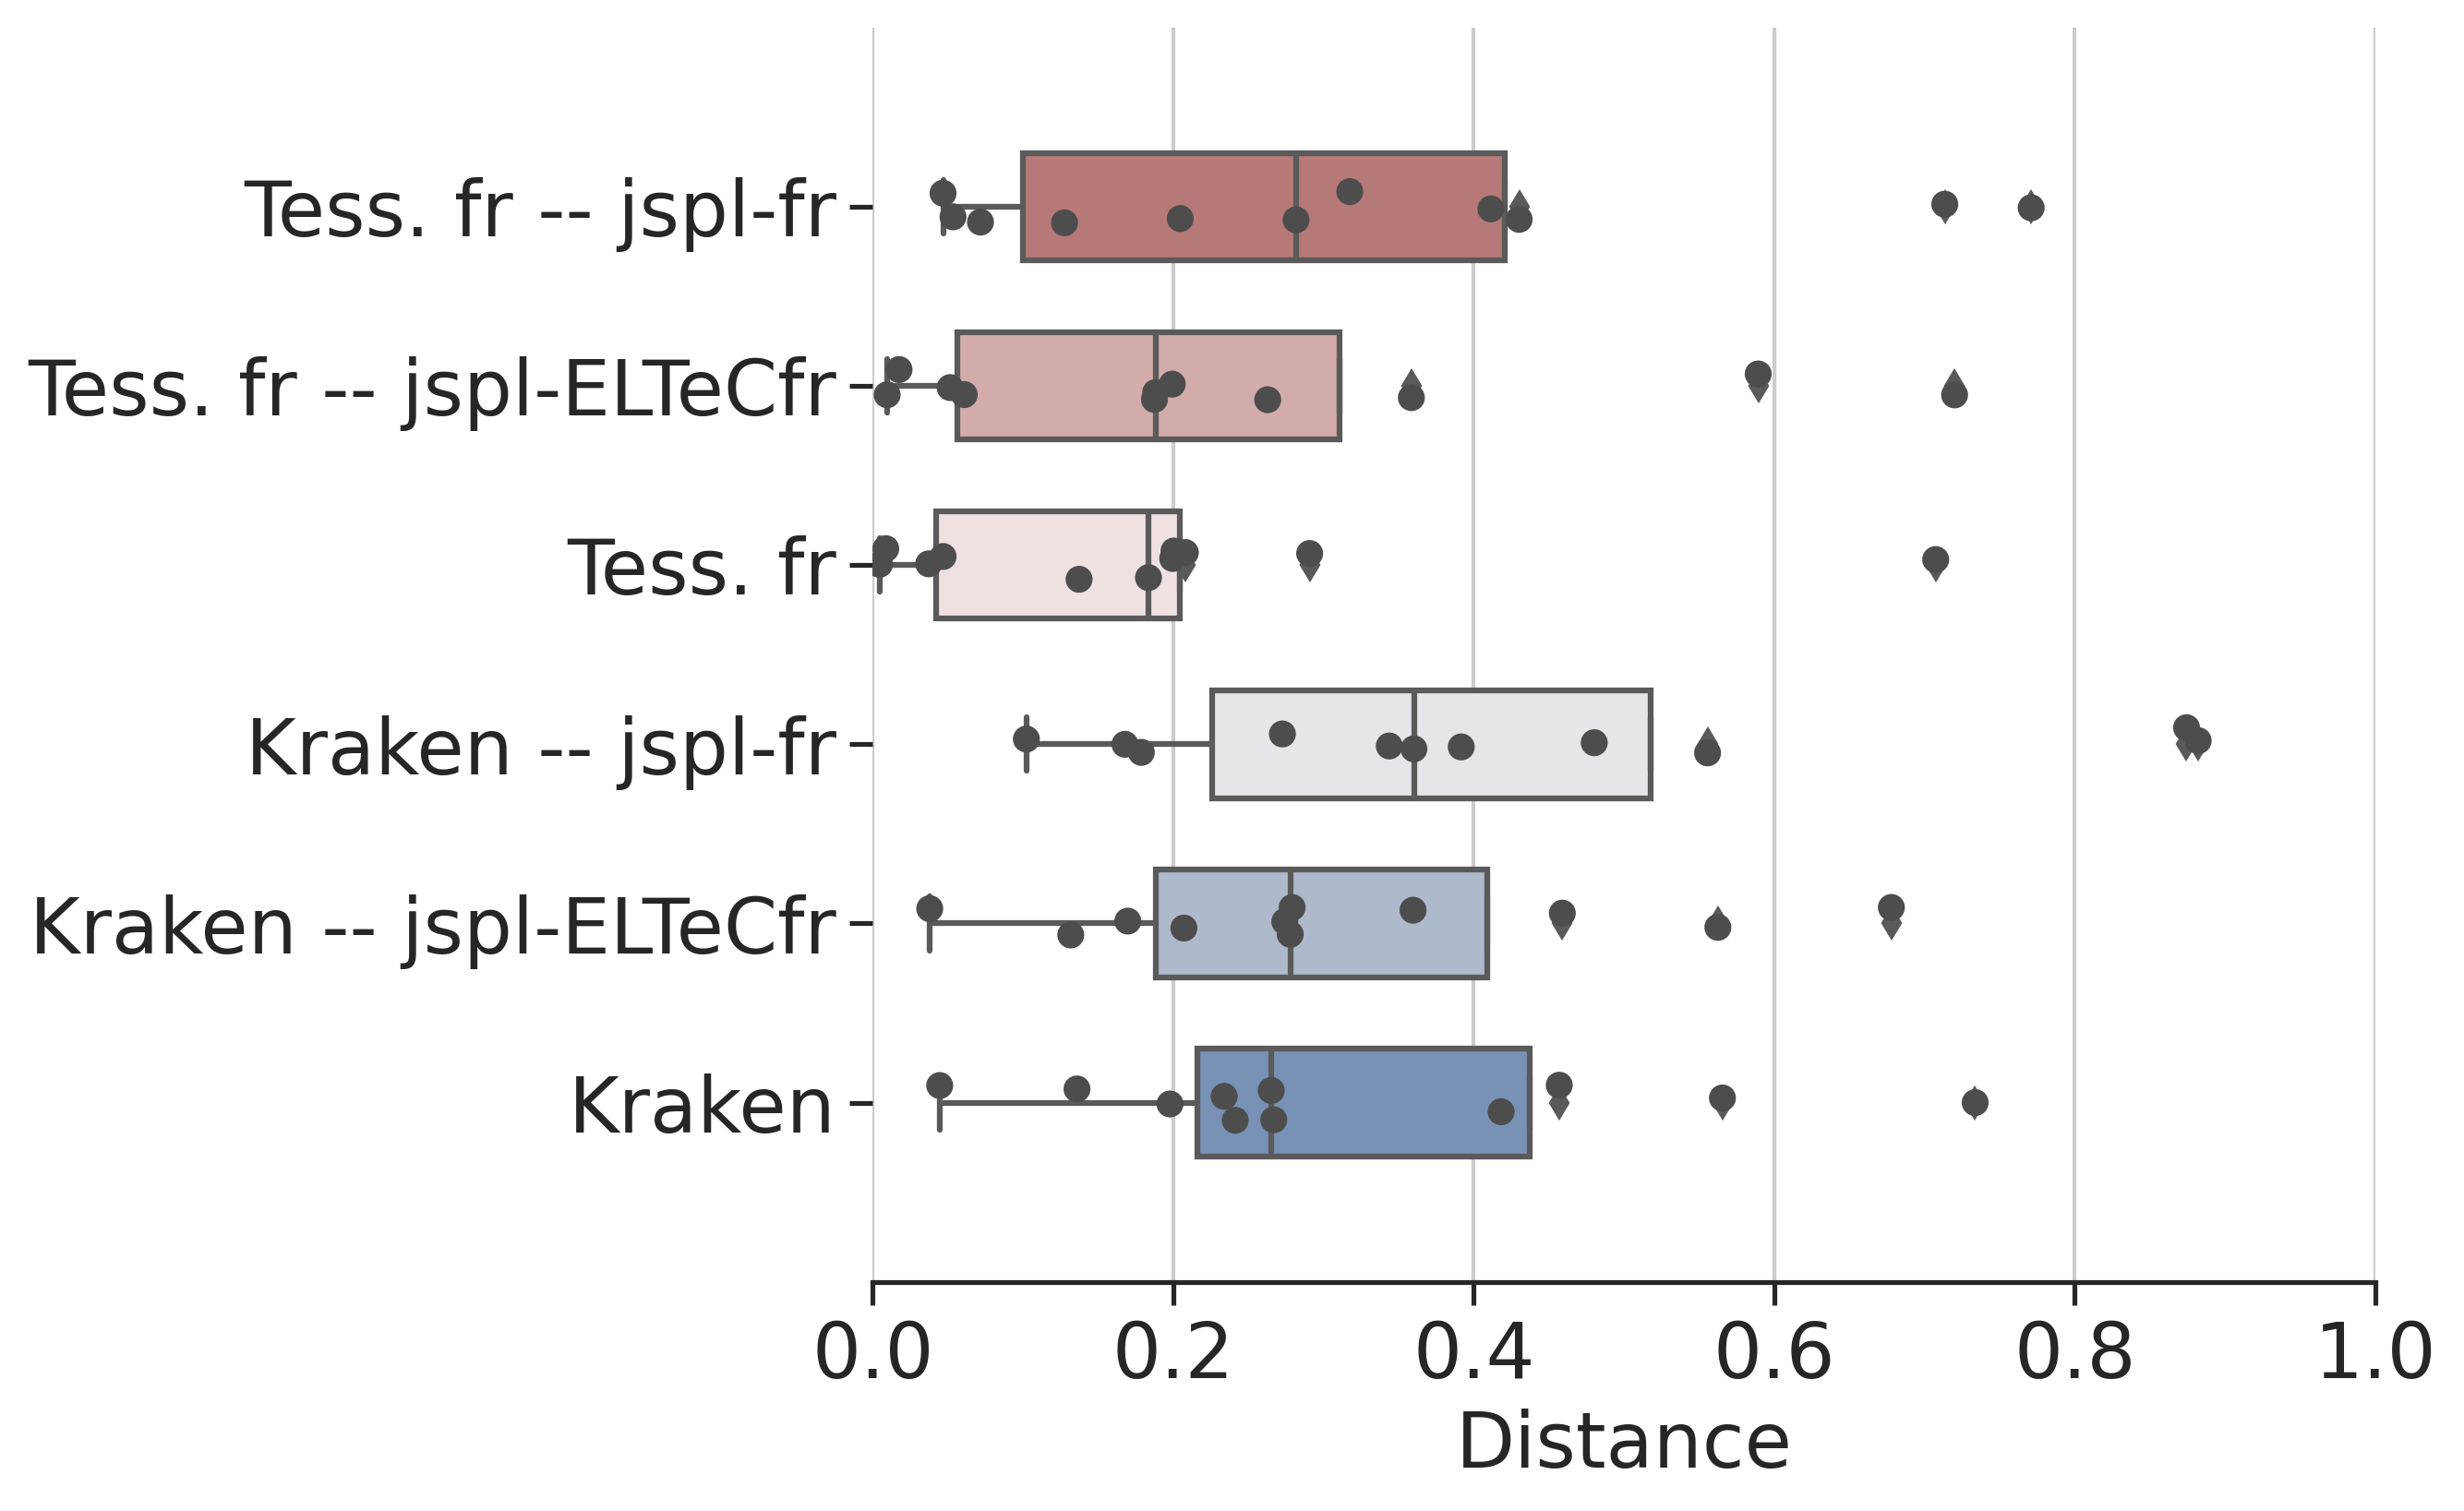
\includegraphics[height=.65\textwidth]{IMAGES/Boite-moustache/ELTeC-Fra_spacy3.5.1_cosinus.png} 
        \caption{ELTeC-Fra \texttt{spaCy} cosinus}
   \end{subfigure}
        \begin{subfigure}{0.5\textwidth}
  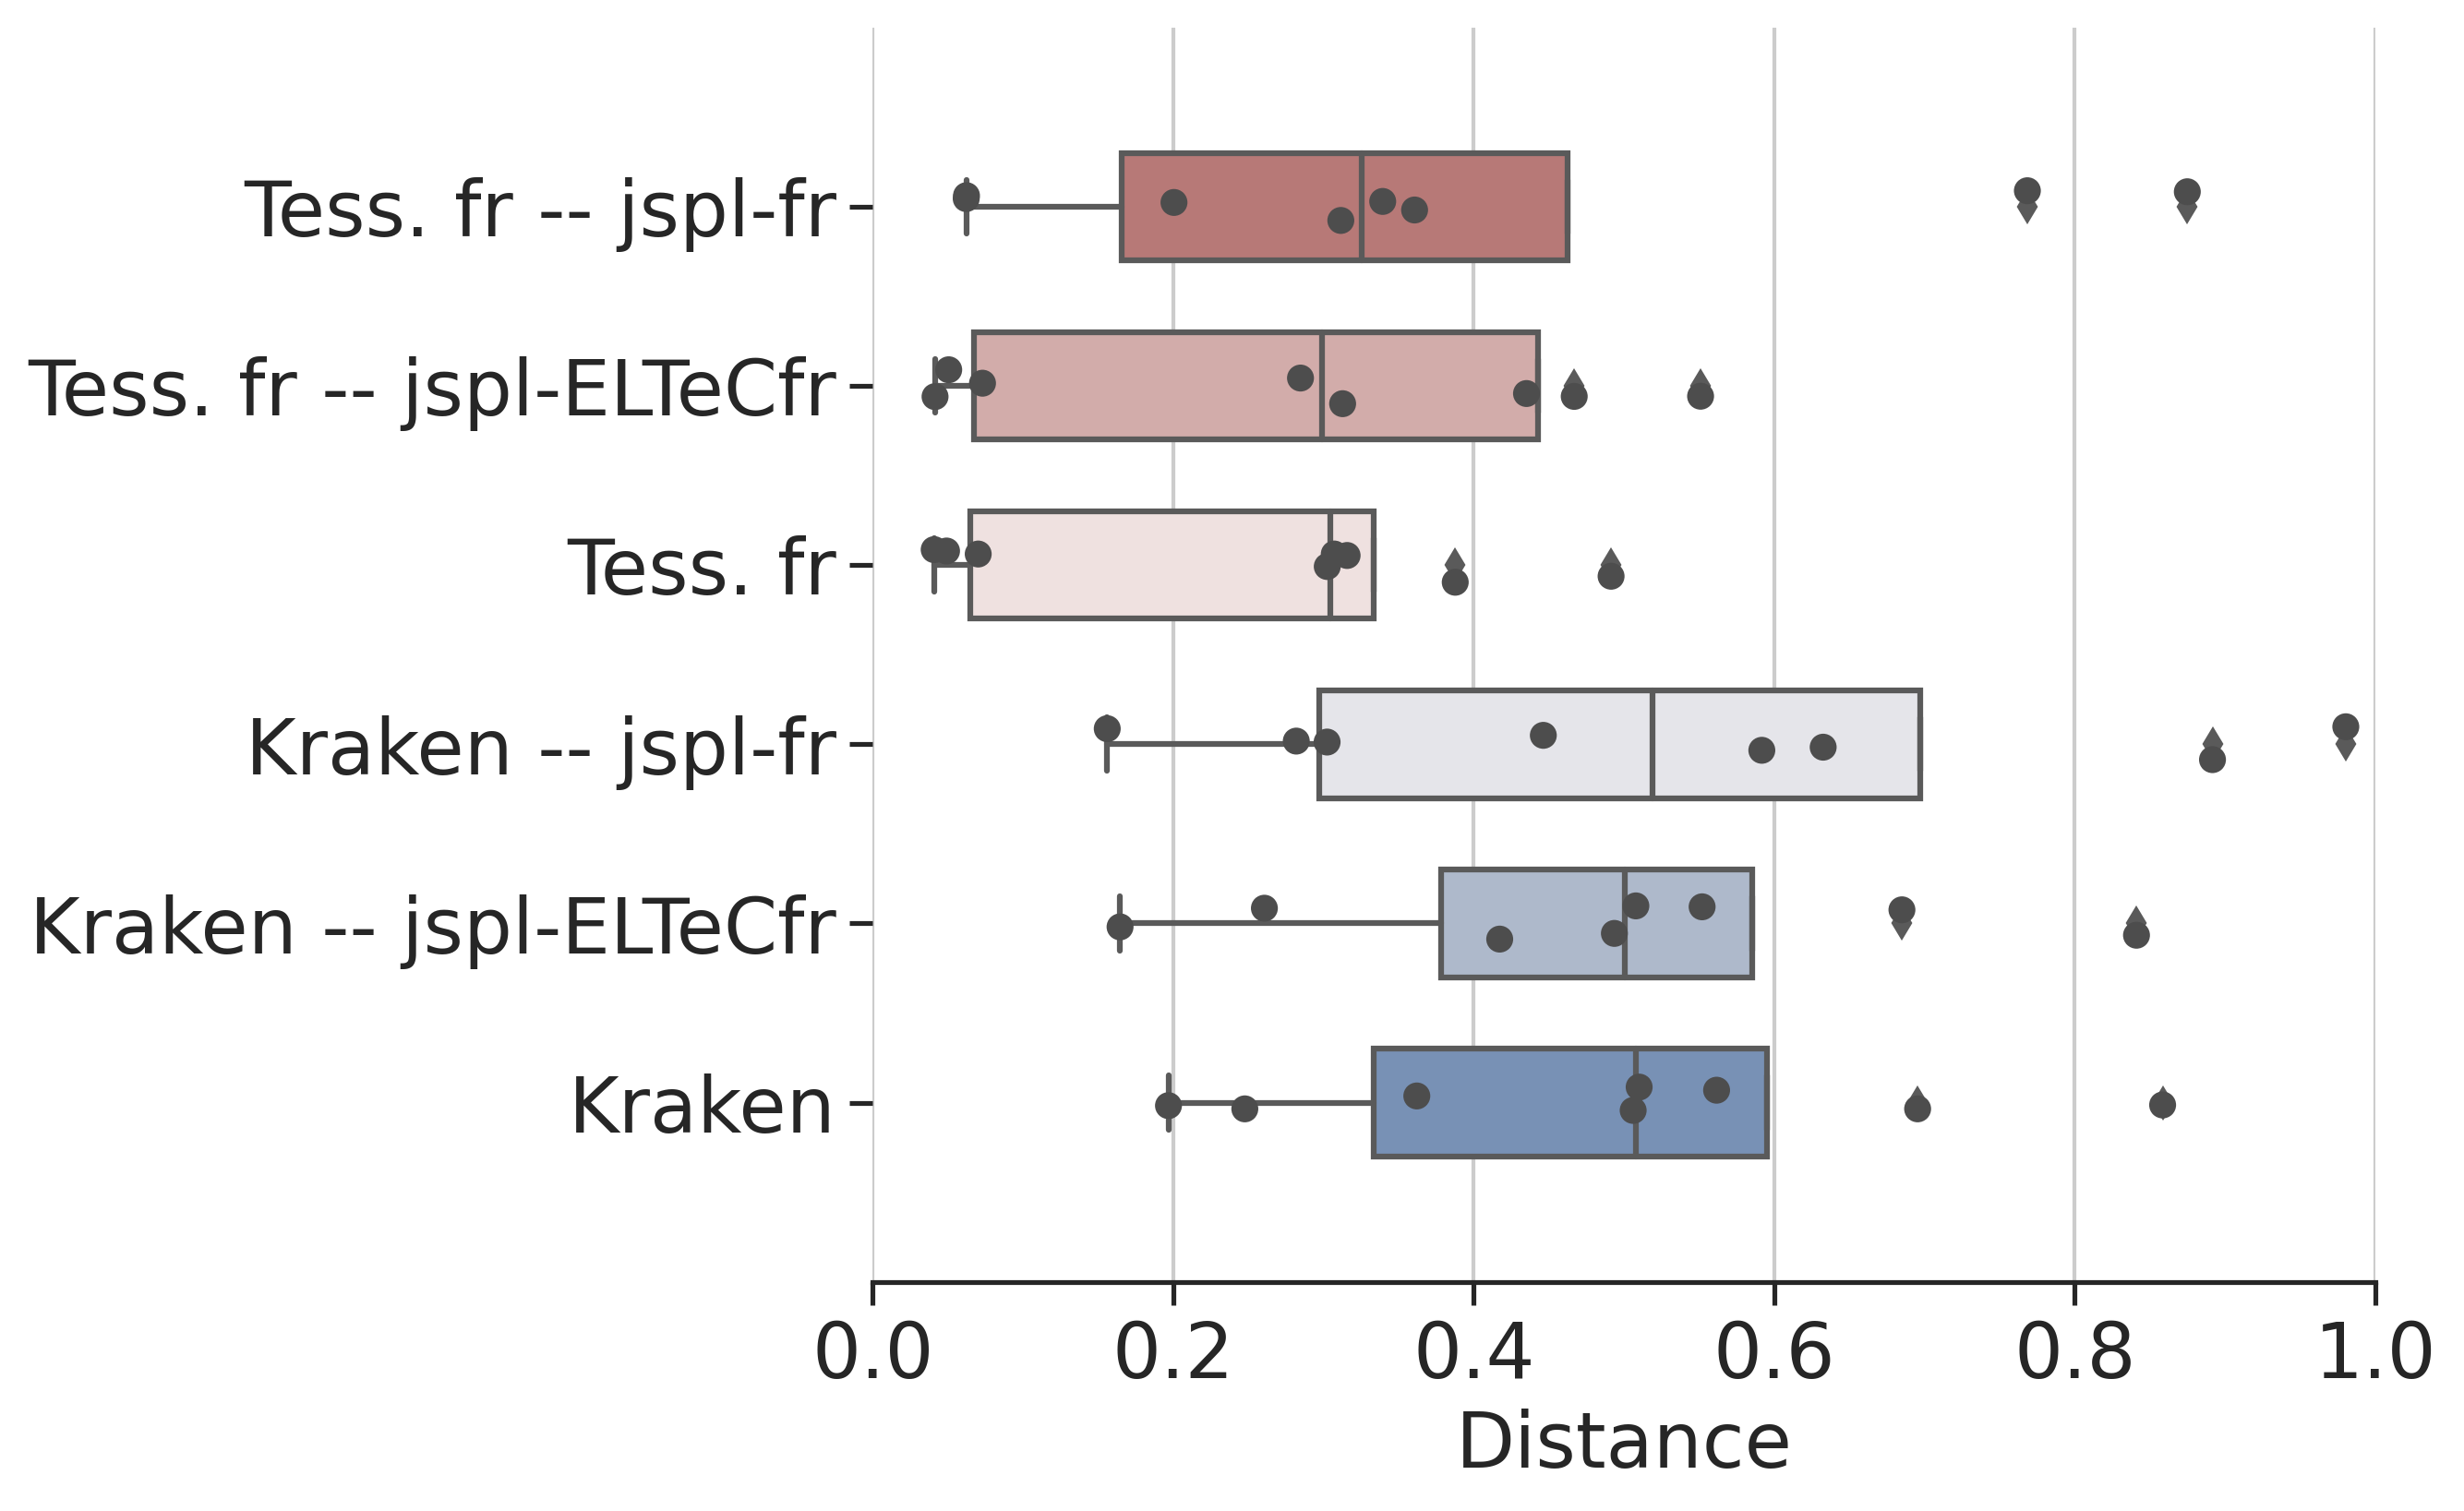
\includegraphics[height=.65\textwidth]{IMAGES/Boite-moustache/TGB_spaCy3.5.1_cosinus.png} 
        \caption{TGB \texttt{spaCy} cosinus}
   \end{subfigure}
   
    \begin{subfigure}{0.5\textwidth}
  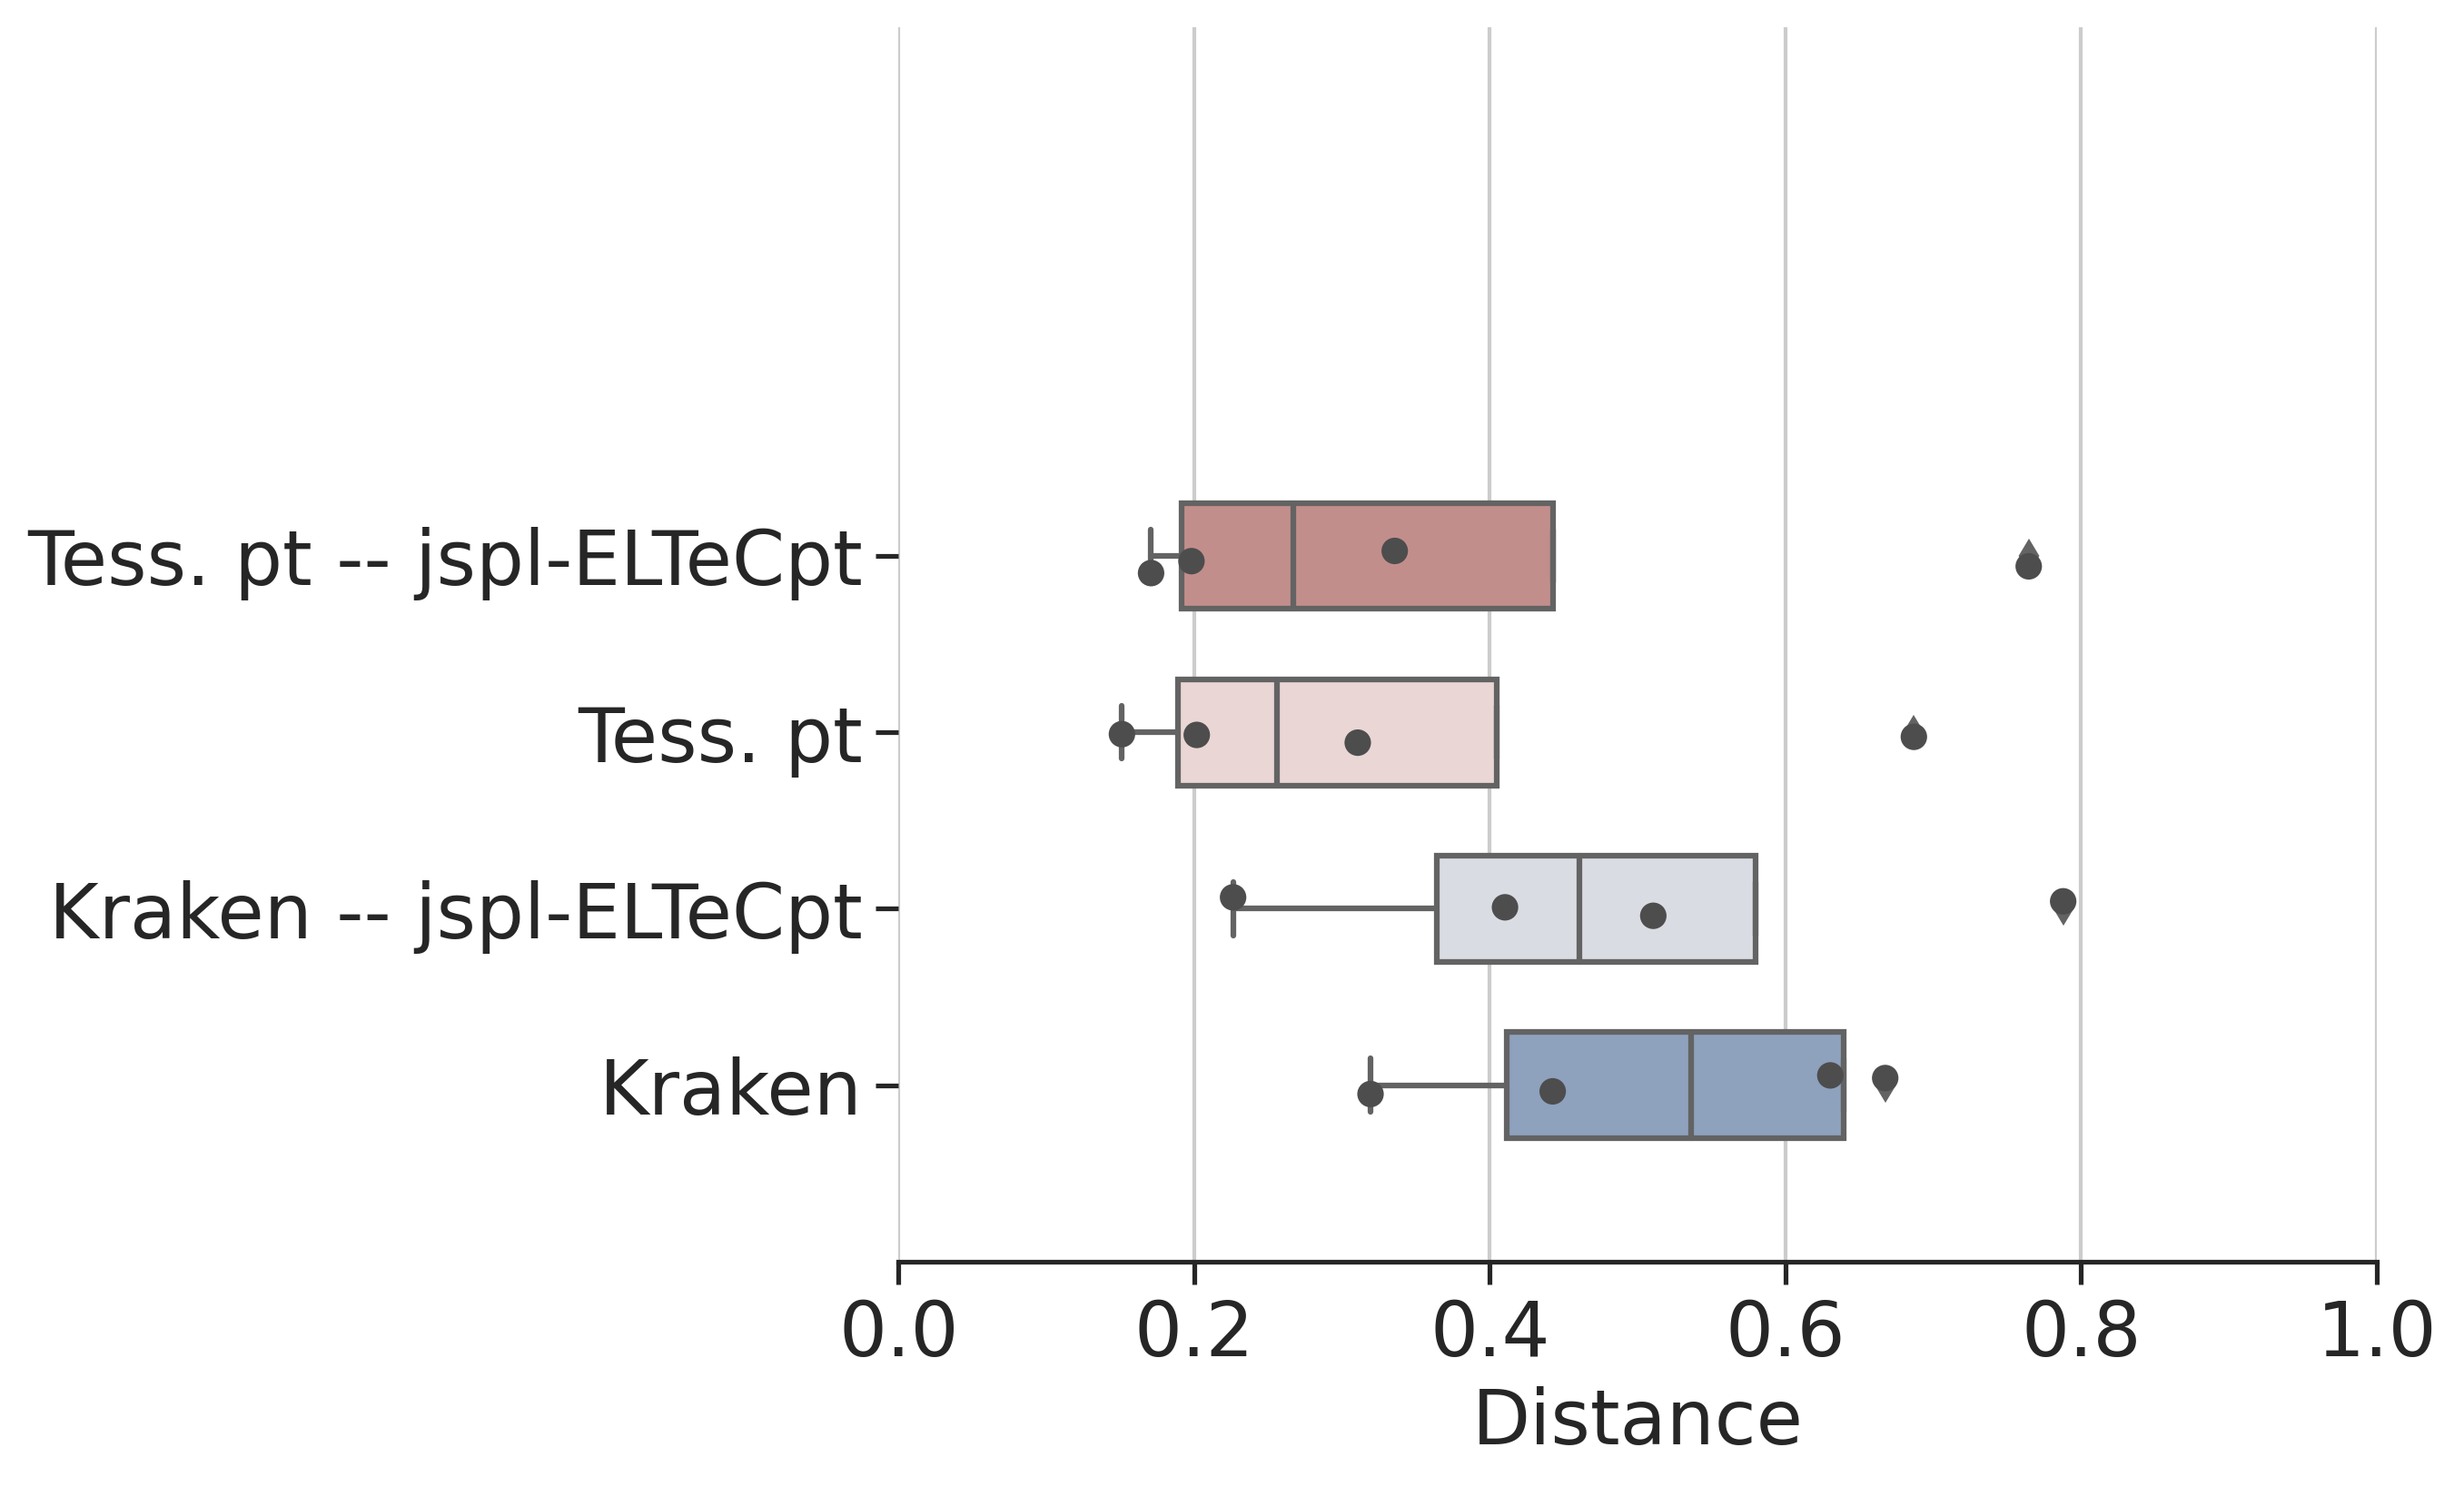
\includegraphics[height=.65\textwidth]{IMAGES/Boite-moustache/ELTeC-Por_spaCy3.5.1_cosinus.png} 
        \caption{ELTeC-Por \texttt{spaCy} cosinus} 
         \label{fig:ELTeC-Por-spaCy-cosinus}
   \end{subfigure}
    \begin{subfigure}{0.45\textwidth}
  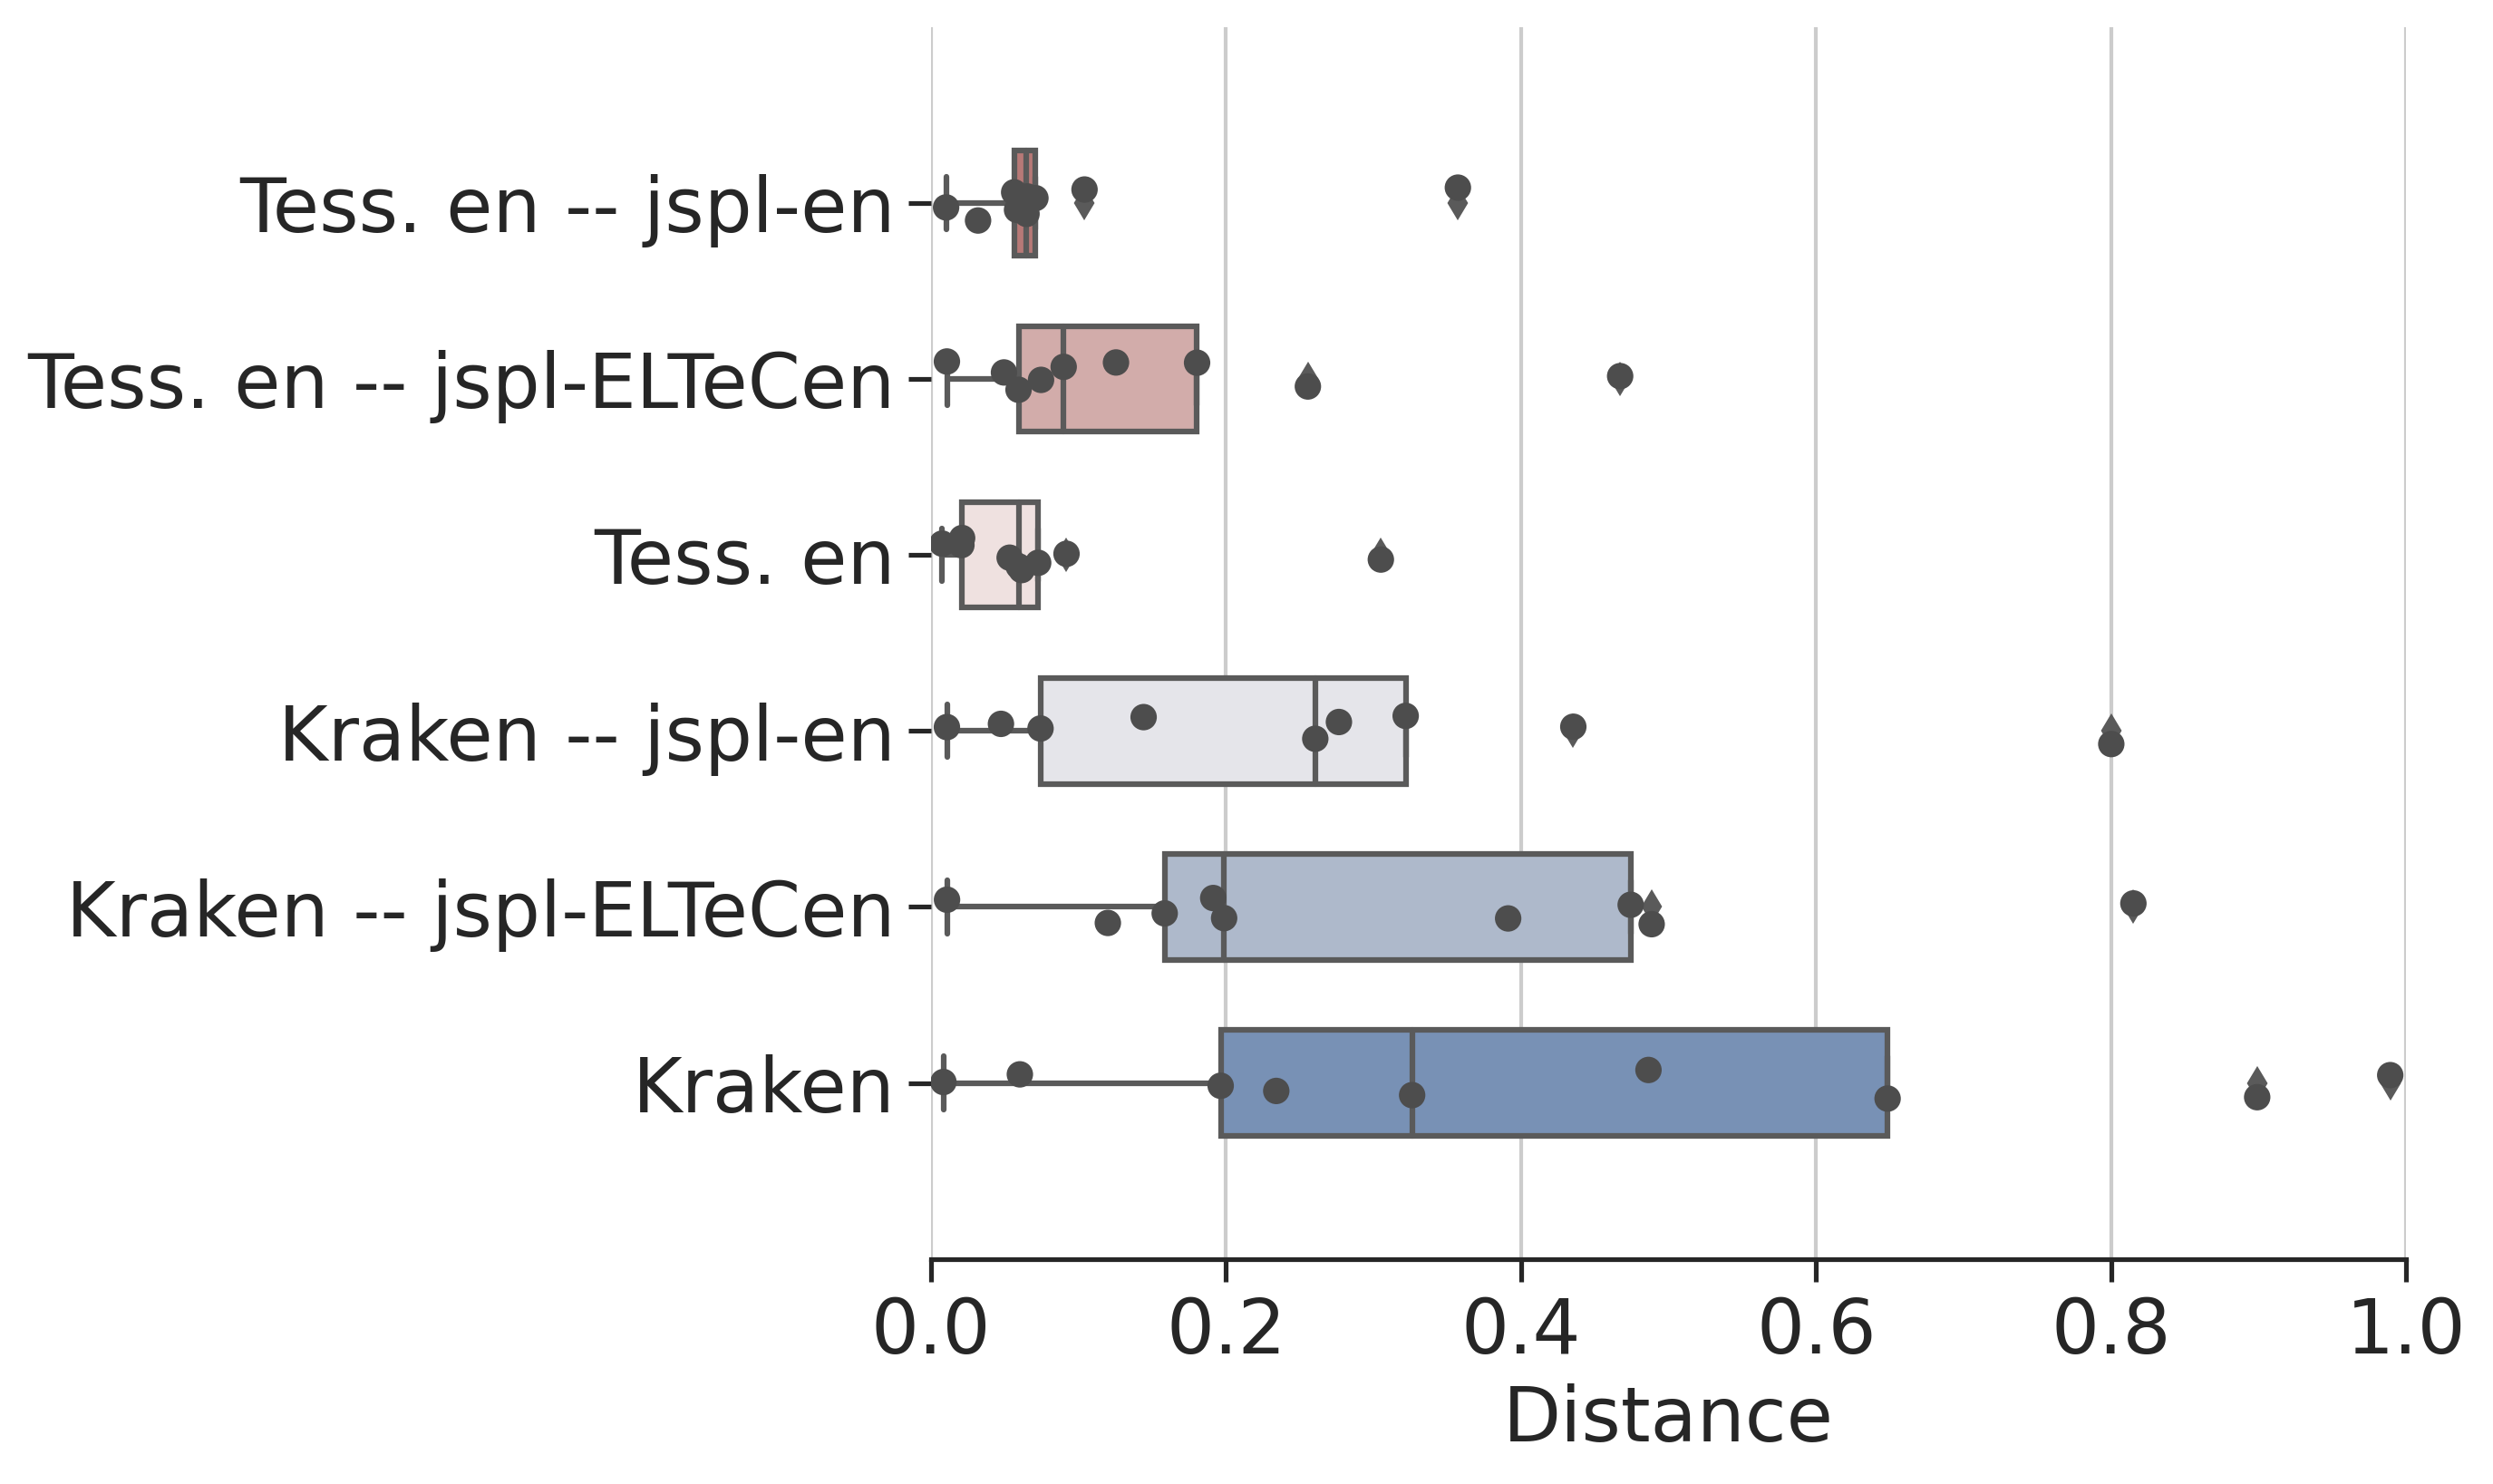
\includegraphics[height=.65\textwidth]{IMAGES/Boite-moustache/ELTeC-Eng_spacy3.5.1_cosinus.png}
        \caption{ELTeC-Eng \texttt{spaCy} cosinus}
   \end{subfigure}

    \caption{Distance Cosinus pour \texttt{spaCy\_lg} sur chaque corpus globalement.}
%    \label{fig:Cosinus-spacy-lg-stanza}
\label{fig:Cosinus-spacy-lg}
\end{figure}


La consultation manuelle des résultats de la REN montre que la différence entre les résultats de Jaccard et cosinus peut s'expliquer par le fait que la première mesure prend en compte le vocabulaire, alors que la seconde s'intéresse au nombre d'occurrences d'une EN. Concrètement, cela signifie pour la distance de Jaccard que si le vocabulaire entre les sorties de deux ensembles comparés est différent même en moindre proportion, le résultat est proche de 1. Pour Jaccard, s'il manque un mot du vocabulaire, cela impactera beaucoup le résultat, alors que pour cosinus ce n'est pas le cas.
En effet, les résultats pour la mesure cosinus dépendent du nombre d'occurrences de chaque EN dans les groupes comparés. Autrement dit, s'il y a beaucoup d'occurrences d'une EN dans la configuration de réf. mais qu'elle n'apparaît pas en même quantité dans la configuration ROC, les résultats pour cosinus grimpent en flèche. L'observation des résultats roman par roman pour la mesure cosinus nous permet d'étayer cette hypothèse, en effet on dénombre, p.\ ex.\, 290 occurrences du terme ``INGLEZA'' pour la configuration Tesseract-pt--\texttt{spaCy\_lg}, alors qu'il apparaît 3 fois seulement dans les résultats de la configuration de réf.\footnote{\textit{Uma familia ingleza}, Diniz.} -- dans ce dernier cas la valeur de cosinus est très élevée et dépasse celle de Jaccard (cos. : 0.69, Jaccard : 0.67). Nous observons un comportement analogue pour chacun des corpus analysés, nous en concluons que la distance de Jaccard a tendance à sur-estimer la distance entre deux ensembles.

La figure \ref{fig:Cosinus-spacy-lg} laisse apercevoir que les résultats de la REN sur les versions Kraken des textes sont moins bons de manière générale que pour les versions produites avec Tesseract. Toutefois, il semblerait que la correction automatique soit un peu plus efficace sur les versions de Kraken avec le modèle Jspll-ELTeC que sur les versions Tesseract, car l'écart entre les boîtes est plus grand. Cependant, les résultats des distances obtenus pour ces versions corrigées de Kraken restent inférieurs à ceux observés pour les versions Tesseract avec et sans corrections. Ces différents constats laissent à penser que plus une version de ROC est bruitée, plus le correcteur automatique intervient et produit de bonnes corrections (figure \ref{fig:ELTeC-Por-spaCy-cosinus}). À l'inverse, si une version de ROC est peu bruitée, alors le correcteur automatique aura tendance à moins bien corriger, voire à sur-corriger. On peut observer ce phénomène concernant les résultats de la REN sur Tesseract qui sont moins bons sur les versions Tesseract corrigées, en le mettant en regard avec nos observations sur le tableau \ref{tab:ELTeC} -- c'est une deuxième manière d'analyser le phénomène de sur-correction. 

%\footnote{Nous analysons les résultats obtenus par ce moteur d'OCR puisqu'il présente moins de fluctuations des valeurs réparties sur les trois catégories de textes -- version non corrigée, version corrigée avec JamSpell pré-entraîné et celle corrigée avec JamSpell ELTeC.} 

%Nous avons identifié une tendance des métriques à illustrer un grand écart entre les valeurs des versions non corrigées et corrigées, notamment dans les figures a.\ et b. Ce \og{}phénomène de creux\fg{} se caractérise par (i) le fait que les mesure de distance de cosinus des versions non corrigées soient bien supérieures à celles de versions corrigées et (ii) que l'écart entre les mesures de distance de soit plus prononcé.

%Enfin, il apparaît en comparant les figures \ref{fig:distances_ref_roc} et \ref{fig:Cosinus-spacy-lg} que la configuration Tesseract--\texttt{spaCy\_lg}, en utilisant pour chacun des outils le modèle de langue adapté à la langue du corpus étudié, soit la plus convaincante en considération du temps de calcul et des résultats. Pour 5 604 472 tokens\footnote{soit le texte brut pour le corpus français de la version de référence et les versions Kraken et Tess. fr.} \texttt{stanza} prend 10 heures à fournir des résultats, alors que \texttt{spaCy} met 1 heure (Mémoire: 16Gio, CPU: Core™i5-1135G7). La lecture des tableaux \ref{tab:EN_contamines_Variantes} et \ref{tab:FP_VP} reportant les analyses manuelles met en évidence des résultats équivalents. 

\subsubsection{\textsc{NERVAL} : Précision, rappel, f-score et effet de seuil}
\label{subsec:NERVAL_COR-OCR-IMPACT-NER}
Dans le but de calculer la précision, le rappel et d'obtenir un f-score nous avons utilisé l'outil \textsc{Nerval}\footnote{\cite{nerval2021}, \url{https://gitlab.com/teklia/nerval}}, évalué par \cite{koudoro2022reconnaissance}. Si cette évaluation présente quelques biais de l'outil, \textsc{Nerval} apparaît tout de même comme un très bon moyen de dépasser les problèmes d'alignements entre les résultats des différentes configurations à comparer pour calculer le f-score. \textsc{Nerval} est développé en Python, et est conçu pour l'évaluation de sorties de REN sur du texte bruité avec la distance de Levenshtein. Les fichiers des textes de référence et des versions de ROC et de ROC corrigées sont annotés au format IOB avec \texttt{spaCy\_lg}. Les fichiers des textes de références ainsi annotés font office de vérité de terrain.
Les premières observations des résultats semblent confirmer que la correction automatique n'est pas forcément un gain pour la REN, en effet le f-score pour les configurations de Tesseract dans les tableaux \ref{tab:NERVAL_DAUDET} et \ref{tab:NERVAL_THACKERAY} perd en moyenne 0.06 points. À l'inverse, le f-score sur les configurations de Kraken semble légèrement augmenter, ce constat venant illustrer le phénomène de creux que nous évoquions dans la partie \ref{subsubsec:seuil}.

\begin{table}[h!]
     \centering
\scriptsize{
\begin{tabular}{|l|r|r|r|r|r|r|}
\hline
 & \multicolumn{2}{c|}{{\# Entités}} & \multicolumn{4}{c|}{\'Evaluation par \textsc{Nerval}}\\
 \hline
Version & ROC & Réf.\ &Intersection& Précision & Rappel & $F_1$ mesure\\

 \hline
Kraken  & 1 122 & 744 &  566  & 0,50    &0,76  &\textit{0,61}  \\
\hline
Tess.fr  & 860 &744  &646     & 0,75     & 0,87  & \textbf{0,81}  \\
\hline
%Tess  & 920  & 944 & 597 & 0.649     & 0.802  & \textit{0.718}  \\
%\hline
\hline
Kraken + Jspll-fr & 1 027  &744  &471     & 0,46     & 0,63  &\textbf{0,53} $\Downarrow$  \\
\hline
Tess.fr + Jspll-fr & 794&  744& 532     & 0,67 & 0,72 & \textit{\textbf{0,69}} $\Downarrow$  \\
\hline
%Tess + Jspllfr &846  & 944 & 503     & 0.595     & 0.676  &\textit{ 0.633 } $\Downarrow$\\
% \hline
\hline
Kraken + ELTeC-fr &1 055 & 744 &548 & 0,52     &0,74  & \textit{0,61} $\Uparrow$ \\
\hline
Tess.fr + ELTeC-fr &838 & 744 & 621  & 0,74     &0,84  & \textit{0,79} $\Downarrow$ \\
%\hline
%Tess + ELTeCfr &927  & 944 &  576    & 0.621     & 0.774  & \textit{0.689} $\Downarrow$\\
\hline
\end{tabular}}
     \caption{Résultat de \textsc{NERVAL} sur {\normalfont Le petit chose}, Daudet.}
     \label{tab:NERVAL_DAUDET}
 \end{table}

   \begin{table}[h!]
     \centering
\resizebox{\textwidth}{!}{
\scriptsize{
\begin{tabular}{|l|l|r|r|r|r|r|r|}
\hline
 & \multicolumn{3}{c|}{{\# Entités}} & \multicolumn{4}{c|}{\'Evaluation par \textsc{Nerval}}\\
 \hline
Version & Label&ROC & Réf.\ &Intersection& Précision & Rappel & $F_1$ mesure\\

 \hline
Kraken  & LOC& 180 & 168&89 &0,50    &0,53 &0,51 \\
Tess. & &161 &168&130&0,81     &0,77&\textbf{0,79} \\
\hline
Kraken &GPE& 1 925 & 1 324& 824&0,43    &0,62 &0,51 \\
Tess. & &1 464 &1 324&1 080&0,74     &0,82&\textbf{0,78} \\
\hline
\hline
Kraken + Jspll-en&LOC & 158 & 168 & 105    &0,67 &0,63&0,64$\Uparrow$ \\ %$\Downarrow$  

Tess. + Jspll-en & & 152&168&119&0,79     &0,71&0,75 $\Downarrow$  
\\
\hline
Kraken  + Jspll-en &GPE&1 542  &1 324&910 &0,59    &0,69 &0,64$\Uparrow$ \\ %$\Downarrow$  

Tess. + Jspll-en  & &1 411 &1 324&1 030&0,73     &0,78&0,75$\Downarrow$ \\
 \hline
\hline
Kraken + ELTeC-en & LOC& 176 &168&99 &0,56    &0,59 &0,58$\Uparrow$\\%$\Uparrow$
Tess. + ELTeC-en& & 158&168&120&0,76     &0,71&0,74 $\Downarrow$\\
\hline
Kraken + ELTeC-en & GPE& 1 149&1 324 &743    &0,65 &0,56 &0,60$\Uparrow$\\%$\Uparrow$

Tess. + ELTeC-en& &1 131 &1 324&868&0,77     &0,66&0,71$\Downarrow$ \\

\hline
\end{tabular}}
}
    \caption{Résultat de \textsc{NERVAL} sur {\normalfont Vanity Fair}, Thackeray.}
     \label{tab:NERVAL_THACKERAY}
 \end{table}

